%===================================================================================================
\if 0
          ,,,,,,,,,,                            lll,,,
          'lllllll'''          ,,llll,,,,,                 ,l,,,,  ''''llll,,,,
           lllllll,       ,,,,,,,,,lllllllllllllll                '''lllll,,,,  ''''lllllllllll
            llllll,,,,,,llllllllllll'''''''''''''                   ,,,,,,   '''lllll,,,,  ''''lllll
    ,,,,,,,,,,,,,,lllllllllllll''''''''''''   lllllllll,,                  '''lllll,,,,   '''lllllllllllll,
,lllllllll''''''''''lllllll,,,,,         ,lllllll'                ll,,,   '''lllll,lllllll, ''lllllll       ,,,,,lllll,
       ,llllllll'''      ,llllllll,,,,,,,,,,,,             ,, '''llll,,,,   '''lllllll,   '   ,,,,,,,llllllllllllllllll
       lllllll,,,       ,,lllll' ''''''llllllllllll,,          ,,llllll,   ''lllllllllll, ,,,ll,,,,,,,llllllllllllllllll''''''' ,lllll
      lllllll''''lllllllll,,,,   ,lllll''     '''''llllllll        ,,llllllllllllll,,,   '''lllll' ''''''''''''ll''''''''       llllll
      ,lllllll   'lllllllll, lll''          ''  ,,,,,,    ,llllllll''  ''''lllllllll    ,l,,   'lllll,,,     llllll,
     ,llllll'    '''''' llllllllll'          ,,,llllllllllllll,llllllll''    ,llllllllllll ,,lllllllll,,,   ''''llll,,,,,,,,,,,, llllll,
    lllll''          lllllll, ,,,,,,,,,,,,lllllllllllll'''''''''''llllllllllll,,   ,,llllllll''  ,,llllllll'''''llllll,,,    '''lllllllll, lllllll
   lllll''     ,,,,,,,,,,,,,,,lllllllllllll''''''''''''       ,,llllllll'' '''lllll,,,llllllll''  ,,llllllll'''  ,,lllllllllll,,,,    '''ll' lllllll,,
  ,l,,,,,,,,lllllllllllll''''''''''''  'lllllll            '''     ,lllllllll''  ,lllllllll''lllll,,,lllllllll' '''llllll,,,     lllllllll,,
  '''''''''''          'lllllll              ''l'll''  ,,llllllll'''   lllllllllll   ,llllllll''lllll,,,,,,,  ''''''''''
              llllll,                   ,,llllllll''   ,lllllllll'''''llllllllllll''   llllllllll,
              lllllll,                  lllllll''   ,llllllll''   ,,lllllllllll,,, ,,lllllll''''
               llllll'                    lllllll''   ,llllllll'  '''llllllllll''
                                       ,,lllllll''   ,llllllll''
                                            ''llll'lll,,,, ,,lllllll'
                                           'lllllllllllll''
                                           ''lllllll'''
\fi
%===================================================================================================

%---------------------------------------------------------------------------------------------------
% preamble
\documentclass{jreport}
% スタイル
\usepackage{sty/graduate}
\usepackage{sty/subfigure}
\usepackage{sty/here}

\usepackage{amsmath}
\usepackage{amssymb}

\usepackage[dvipdfm]{graphicx}

\usepackage[dvipdfm]{color}
\usepackage[T1]{fontenc}
\usepackage[varg]{txfonts}
% 箇条書き
\usepackage{enumerate}
% 太字
\usepackage{bm}
% 表の行結合
\usepackage{multirow}
\usepackage{url}
\usepackage{array}

\newcommand{\bhline}[1]{\noalign{\hrule height #1}}   

\normalfont
\pagestyle{plain}
\title{NDTを用いたステレオカメラによる\\移動ロボットの自己位置同定手法の開発}
\author{李 珍鎬}
\date{平成28年2月}
\major {電気情報工学科}
\department{九州大学工学部電気情報工学科}

%---------------------------------------------------------------------------------------------------
% document
\begin{document}
\maketitle
%===================================================================================================
% 序論
%===================================================================================================
\chapter{序論} 
%---------------------------------------------------------------------------------------------------
\section{背景}
近年,少子化や高齢化のため,労働力不足の問題が深刻化している.この労働力不足の対策案として自律移動ロボットや無人搬送車,あるいは自動運転技術の開発が進められている.自律移動ロボットや自動運転技術が実現されることにより,労働力不足への対策のみならず,人の移動の効率化や交通事故の防止にも繋がると期待が寄せられている.自律移動ロボットや自動運転技術の実現には,高精度な位置同定と移動中の障害物回避技術が必要不可欠となる.そこで,本研究では移動ロボットの高精度な位置同定に注目する.
移動ロボットが自己位置推定を行う方法としては大きく環境地図が利用できない場合と利用できる場合に分けられる.環境地図が利用できない場合は,車輪の回転角度を積分し移動量を推定するオドメトリ,GPSなどの方法がある.環境地図が利用できる場合は外界センサ(レーザーやステレオカメラなど)の計測データと環境地図との比較をして自己位置推定を行う.

しかし,従来の自己位置推定方法にはいくつかの問題がある.オドメトリは車輪の滑り検出が難しかったり,誤差が起きると誤差が累積される問題がある.GPSは屋内など屋根があるところでは正確に自己位置推定ができない.環境地図が利用できる場合は累積誤差は小さいが,特に3次元位置同定の場合,3次元環境地図と外界センサの3次元計測データとの比較であるため,計算コストが莫大になる問題が生じる.そこでこれまでに,環境地図が利用できる場合の計算コストの問題をNormal Distribution Transform(NDT)を利用して解決した,RGB-Dカメラ(Kinect)を利用した高速な位置同定法[1]が提案されている.

\newpage
%---------------------------------------------------------------------------------------------------
\section{本研究の目的}

文献[1]では,代表的なRGB-DカメラであるKinectを用いて屋内の位置推定を行ってきたが,Kinectの性能上,屋外での位置推定は難しい.そこで,本研究では,屋外でも計測が可能なステレオカメラを用い,ステレオカメラから得られる3次元データを用いたNDTによる屋内・屋外の位置推定を目標とする.
%---------------------------------------------------------------------------------------------------
\section{概要}

本研究では,屋内のみならず,屋外環境でステレオカメラを用いた場合でも,従来提案されているNDTを用いた位置同定手法を適用することで,高速で高精度な移動ロボットの位置同定が可能であることを示す.このために以下の課題に対して検討を行う.

1つ目は,ステレオカメラを用いたNDTによる位置同定の可能性の検討である.前述の通り,ステレオカメラを用いたNDTによる位置同定は行われておらず,実際の屋内環境でどこまで位置同定できるかを検討する.
2つ目はステレオカメラの性能に関わるテクスチャー有無やボクセルの解像度,オーバーラップの有無などの各条件による精度と計算コストを比較し,最適な計測条件について検討する.ここで得られた最も効率的な条件を基にしてKinect V2との精度比較,屋外位置同定を行う.
最後は,屋外での適用可能性の検討である.移動ロボットに適用するためには屋内だけでなく屋外でも利用できなければならないため,ステレオカメラを用いた屋外位置同定の可能性について検討する.
%
\newpage
%---------------------------------------------------------------------------------------------------
\section{本論文の構成}
本論文はまず,NDTを用いた位置同定について述べてから,ステレオカメラを用いた位置同定について述べる.
次に計測実験と評価について述べた後,最後に本研究のまとめと今後の課題を述べる.

以下に本論文の構成を示す.
\begin{description}
 \item[第1章] 本研究の背景,目的,概要について述べる.
 \item[第2章] NDTを用いた位置同定について述べる.
 \item[第3章] ステレオカメラを用いた位置同定について述べる.
 \item[第4章] 計測実験と評価について述べる.
 \item[第5章] 本研究のまとめと今後の課題について述べる.
 \end{description}

%===================================================================================================
%
%===================================================================================================
\chapter{NDTを用いた位置同定}
%---------------------------------------------------------------------------------------------------
\section{概念}
第1章では,様々な位置同定の方法と問題点について述べた.その中でも,本研究ではステレオカメラを用いた3次元計測データと地図データを利用したNDTによる位置同定法について検討する.
NDTとは,Normal Distribution Transformの略語である.文献[1]では,NDTにより生成されるデータとして,ND Voxelと代表平面,および7つの代表点を用いた.また確率的な位置の同定手法としてパーティクルフィルタを用いた.パーティクルフィルタを用いて地図データと計測データとの尤度計算を行い,位置同定する.第2章ではNDTを用いた位置同定について説明し,NDT,パーティクルフィルタの概念について述べた後,実際の位置同定を行うシステムの流れについて述べる.

\newpage
%
%---------------------------------------------------------------------------------------------------
\section{Normal Distribution Transform(NDT)}
NDT(Normal Distributions Transform)とは空間を格子状に分割し,それぞれの格子内に含まれる観測点群の位置に対して分散行列を求め,固有値分解することで得られる分散値による3次元正規分布で空間を表現する手法である.NDTの概念を図{\ref{NDTの概念}}に表す.前述した通り,NDTにより生成されるデータとして,文献[1]ではND ボクセルと代表平面,および7つの代表点を用いている..\par
まず,NDボクセルとはNDTにより得られた正規分布と平均値を与えた一つの3次元格子を言う.ある点$x_{i}$=($x_{i}$,$y_{i}$,$z_{i}$)とすると,どのボクセルに入っているかを座標値を量子化することで求める.次に,求められたボクセルをボクセルkとすると,ボクセルkに入っている$N_{k}$個の点を$x_{k}$(i=0...$M_{k}$-1)とする.このとき,ボクセルkの平均点$m_{k}$と共分散$ \Sigma_{k} $を以下のように求める.\par

\begin{equation}
m_{k}=\cfrac{1}{N_{k}}\sum_{i=0}^{N_{k}-1}x_{ki}
\end{equation}
\begin{equation}
\Sigma_{k}=\cfrac{1}{N_{k}}\sum_{i=0}^{N_{k}-1}(x_{ki}-m_{k})(x_{ki}-m_{k})^t
\end{equation}

%
\begin{figure}[htbp]
  \vspace{-3mm}
  \begin{center}
   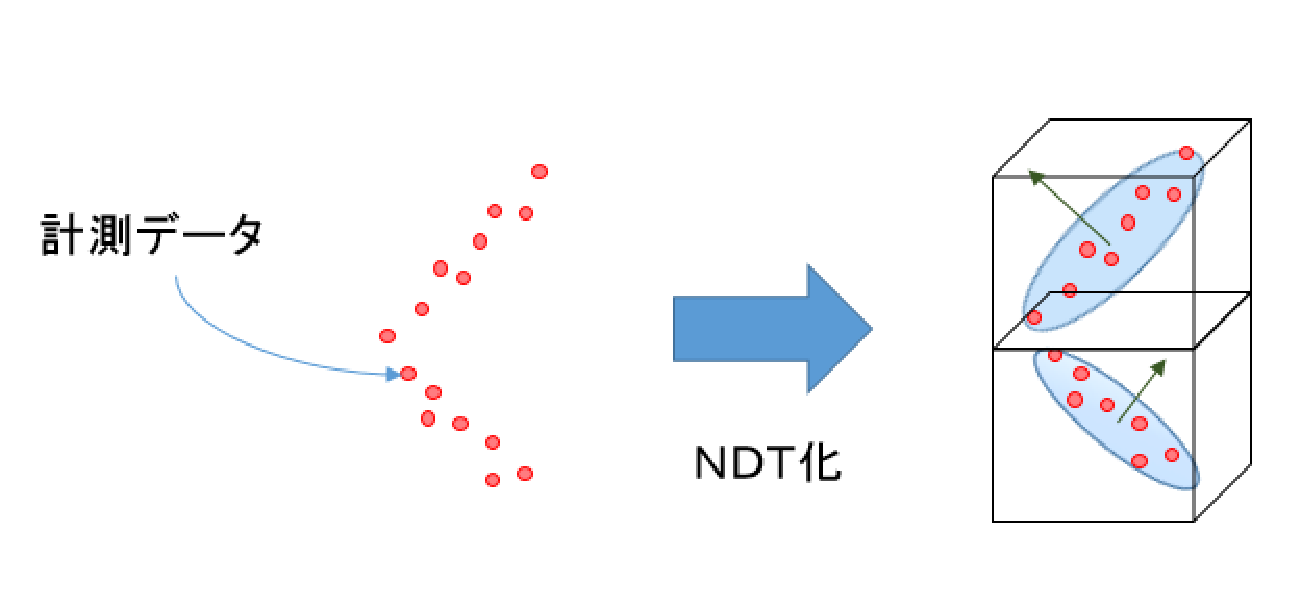
\includegraphics[height=55mm]{figure/NDTの概念.eps}
   \vspace{-5mm}
   \caption{NDTの概念}
   \label{NDTの概念}
  \end{center}
\end{figure}
%
\newpage
%
代表平面とは,各ボクセルにおいて,計算された3次元正規分布から分散値が最も小さい方向を法線ベクトルとする平面を言う.図2.1で説明すると,赤い点が計測された点群で,図2.1の右側にある格子がND ボクセル,また,青い楕円型が代表平面で緑色の矢印が代表平面の法線ベクトルである.\par
7つの代表点とは,得られた三次元正規分布に対して,各軸方向に半径$\sqrt{-2\ln \gamma}$の球面上の点を楕円上に射影した点6つと正規分布の中心点を合せた7つの点を言う.本研究では7つの代表点は計測データからのみにできるものとしている.つまり,地図データにはND ボクセルと代表平面,計測データにはND ボクセルと代表平面に加えて7つの代表点がある.データ構成を図{\ref{データ構成}}に表す.また,NDTにより得られる代表平面,代表点を図{\ref{NDTまとめ}}に表す.
%
\begin{figure}[htbp]
  \vspace{-3mm}
  \begin{center}
   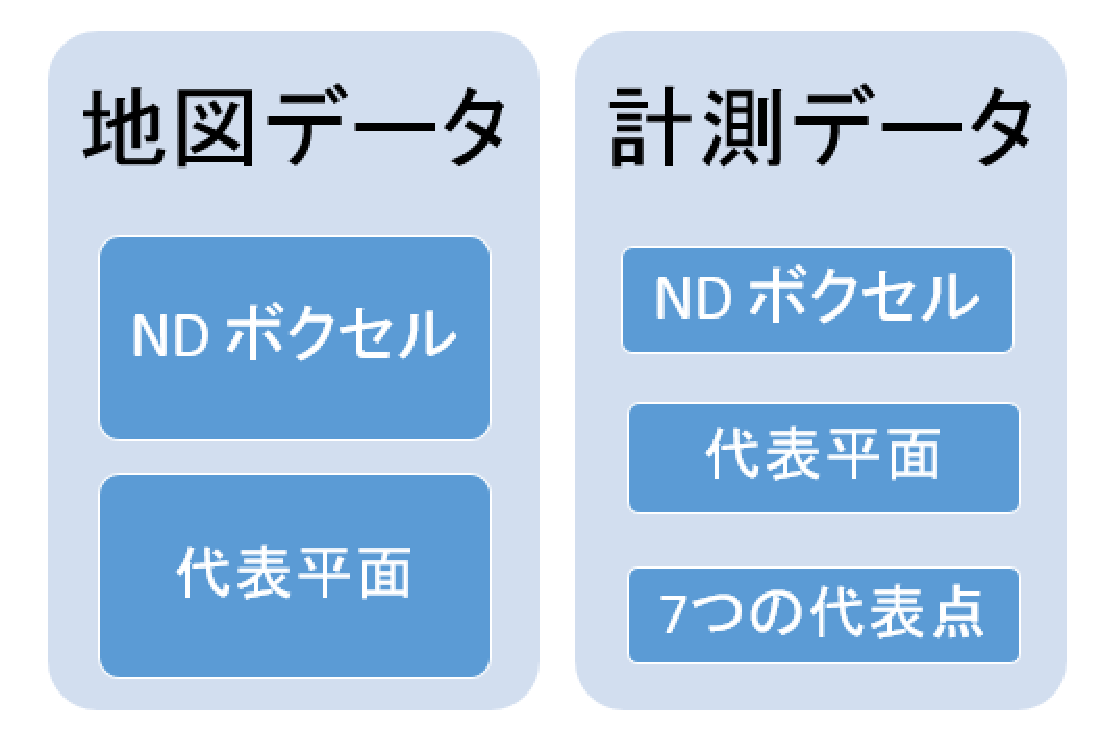
\includegraphics[height=55mm]{figure/データ構成.eps}
   \vspace{-5mm}
   \caption{データ構成}
   \label{データ構成}
  \end{center}
\end{figure}
%

%
\begin{figure}[htbp]
  \vspace{-3mm}
  \begin{center}
   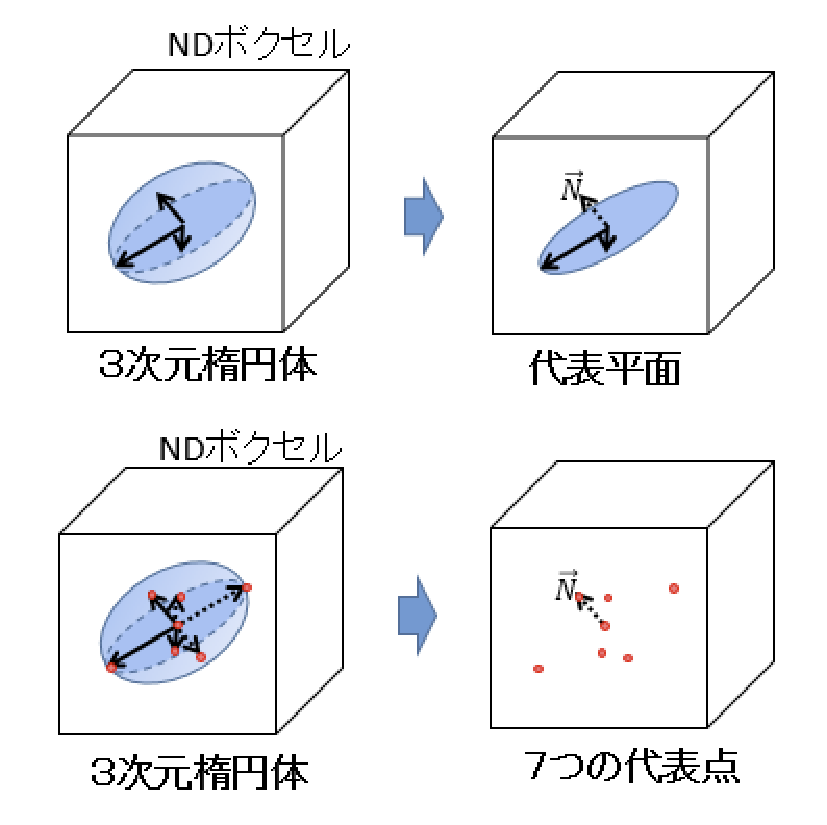
\includegraphics[height=65mm]{figure/NDTまとめ.eps}
   \vspace{-5mm}
   \caption{NDTまとめ}
   \label{NDTまとめ}
  \end{center}
\end{figure}
%

\newpage
%
しかし,NDTを利用してデータの簡略化はできるが,格子内に区切る離散化の影響により,境界付近に存在する点群形状が隣のボクセルで確認できないことがあり得る.対象ボクセルとその周りのすべてのボクセルとマッチング評価を行えば解決できるが,周りのすべてのボクセルは計27であるため,計算量が多くなるという問題がある.そこで,本研究では離散化の影響を低減するため,オーバーラップND ボクセルを用いる.オーバーラップND ボクセルとは,Biberら[3]の手法を3次元に拡張し,各格子を半分ずつ重複するようにし,1つの点が8つのボクセルに含まれるようにする手法である.図{\ref{オーバーラップNDボクセル}}にオーバーラップ NDボクセルの概念を表す.また,オーバーラップ NDボクセルの例を図{\ref{オーバーラップNDボクセルの例}}に表す.

%
\begin{figure}[htbp]
  \vspace{-3mm}
  \begin{center}
   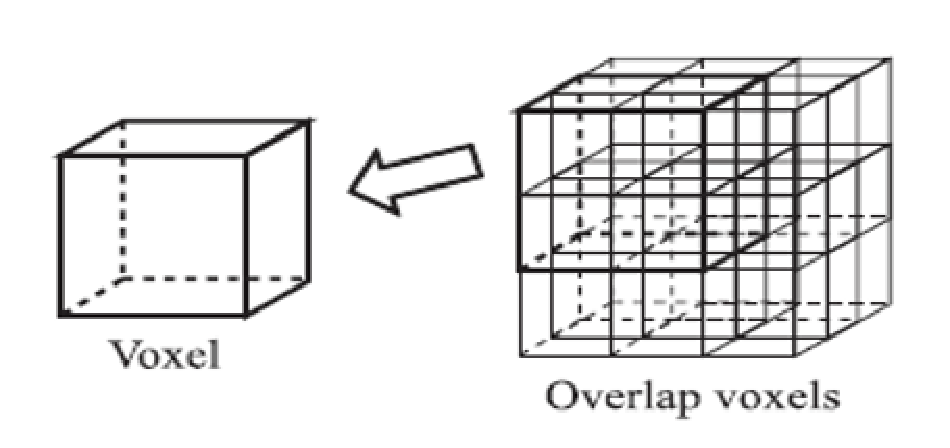
\includegraphics[height=55mm]{figure/オーバーラップNDボクセル.eps}
   \vspace{-5mm}
   \caption{オーバーラップNDボクセル([1]より引用)}
   \label{オーバーラップNDボクセル}
  \end{center}
\end{figure}
%
%
\begin{figure}[htbp]
  \vspace{-3mm}
  \begin{center}
   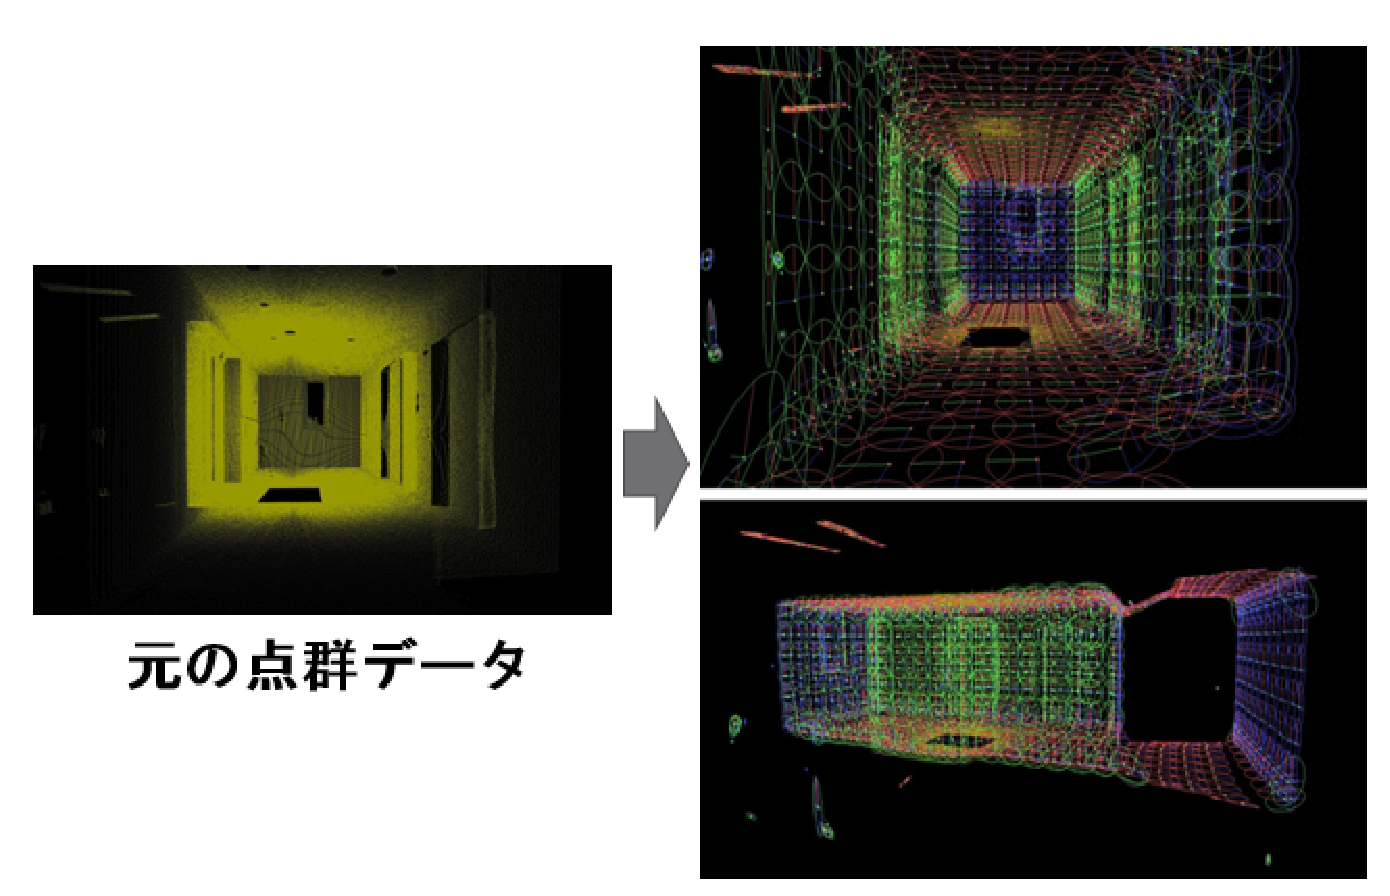
\includegraphics[height=55mm]{figure/オーバーラップNDボクセルの例.eps}
   \vspace{-5mm}
   \caption{オーバーラップNDボクセルの例([1]より引用)}
   \label{オーバーラップNDボクセルの例}
  \end{center}
\end{figure}
%
\newpage
%
NDTによりできるND ボクセルには大きさがあり,大きさを変えることでデータの解像度が変わる.ボクセルの大きさを小さくするほど,解像度は良くなるが,計算時間が増える.したがって,状況によってボクセルのサイズは変える必要がある.ボクセルのサイズによる解像度の例を図{\ref{ボクセルサイズによる解像度}}に表す.

\begin{figure}[htbp]
  \vspace{5mm}
  \begin{center}
   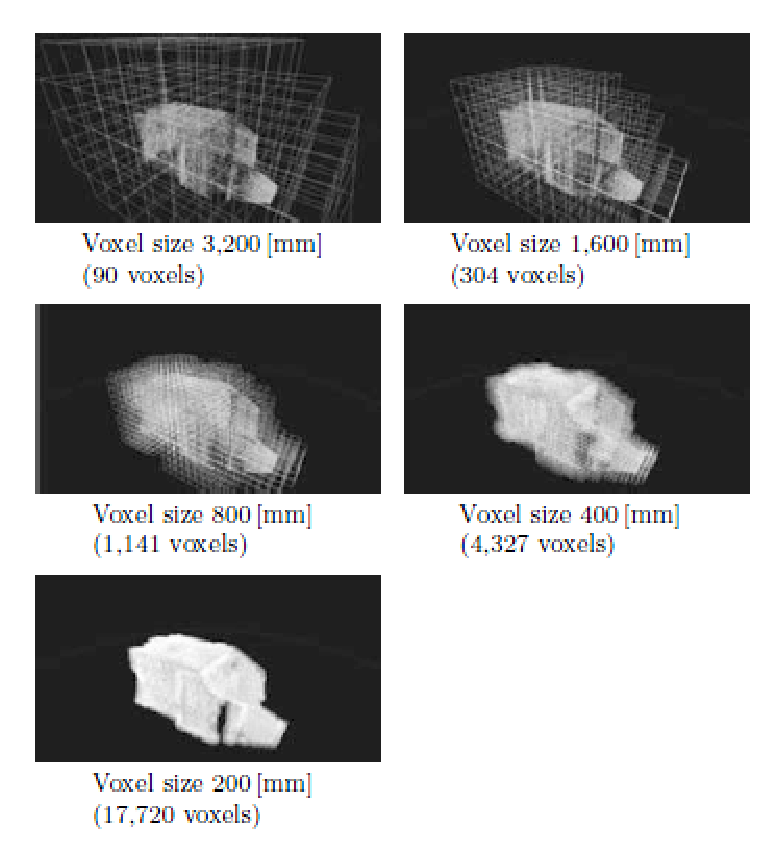
\includegraphics[height=120mm]{figure/ボクセルサイズによる解像度.eps}
   \vspace{-5mm}
   \caption{ボクセルサイズによる解像度([1]より引用)}
   \label{ボクセルサイズによる解像度}
  \end{center}
\end{figure}
%
\newpage
%
%---------------------------------------------------------------------------------------------------
\section{パーティクルフィルタ}
NDTにより3次元データの簡略化を行い,位置同定にはパーティクルフィルタを用いる.フィルタとは与えられた物から特定成分を取り除くまたは弱める作用をする機能を言う.ここで特定成分とはデータに含まれたノイズなどを含め,不確実性のデータをフィルタリングし正しい結果を推定することである.本研究ではパーティクルフィルタを用いて地図データの中から計測データと合致する位置を推定する.まずは,地図データ全体に決まった数のパーティクルをばら撒く.ばら撒いたパーティクルには重みと状態量があって、最初の位置から次の位置まで移動量を予測する.その次に前状態の情報を用いて移動方向に対して尤度(もっともらしい値)を計算する.そこで,ある基準からパーティクル尤度の値が低かったら,そのパーティクルは削減される.またパーティクル尤度の値が大きいほど,その周りにはパーティクルが集中するようになる.集中されたパーティクルを用いて同じ過程を繰り返し,最終的に収束される位置が推定する位置となる.本研究のパーティクルフィルタの流れを簡単にまとめる.
\begin{enumerate}
\item 初期化:パーティクルを位置・姿勢地図データ全体にランダムにばら撒く.4に進む.
\item リサンプリング:以前時刻のパーティクルのうち一つのその重みを確率としてランダムに選択し,指定された最大パーティクル数分繰り返し選択する.
\item 予測:選択された各々のパーティクルに対してシステムの動作モデルを適用し,現時刻のシステムの状態(位置・姿勢)を予測する.
\item 尤度計算,重み付け:測定情報と各々のパーティクルの状態から評価関数によって尤度計算を行い,その結果を新たな重みと付ける.
\item 2に戻る.
\end{enumerate}

\newpage
%
%---------------------------------------------------------------------------------------------------
\section{地図データと計測データとのマッチング(尤度計算)}
ND ボクセルで表された地図データと計測データを用いて,パーティクルフィルタにより位置追跡を行う.各パーティクルには各々候補となるロボットの位置t,姿勢Rを持つ.尤度計算手順の流れを図{\ref{尤度計算手順}}に表す.\par

\vspace{10mm}
\begin{figure}[htbp]
  \begin{center}
   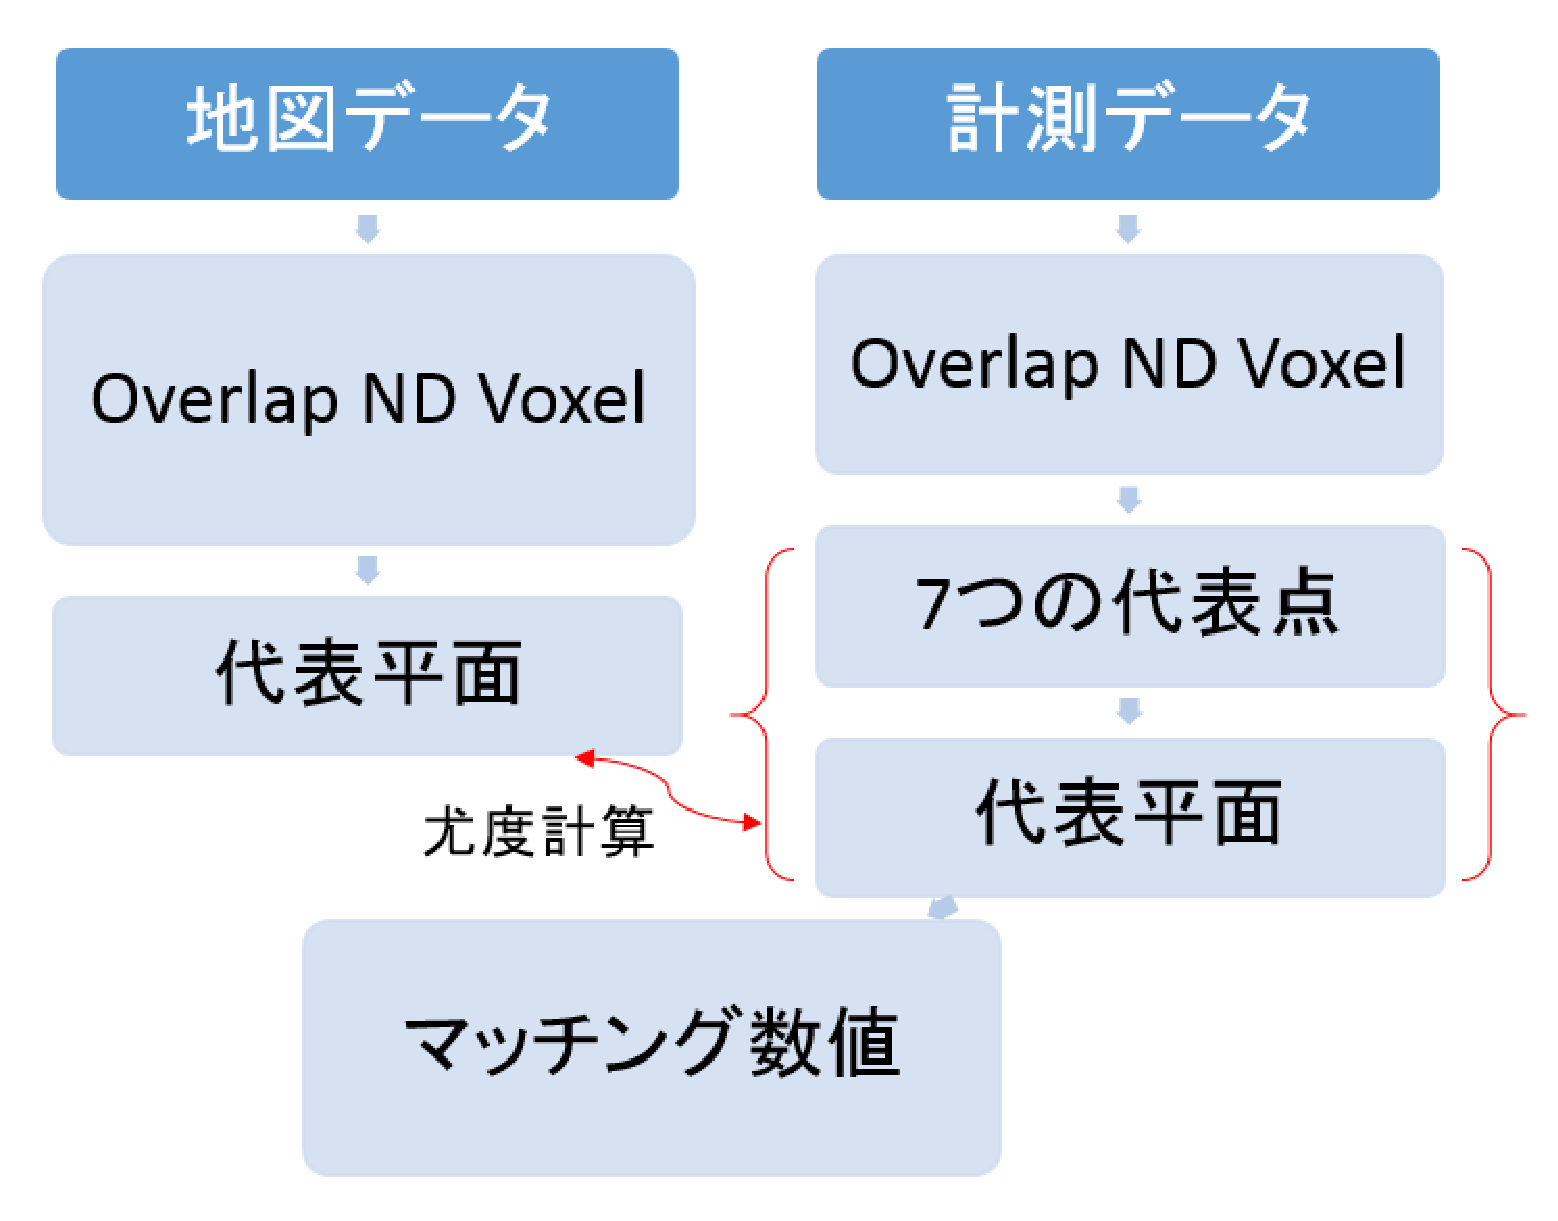
\includegraphics[height=70mm]{figure/尤度計算手順.eps}
   \caption{尤度計算手順}
   \label{尤度計算手順}
  \end{center}
\end{figure}
%
まず,計測データ中の各ボクセルを位置姿勢候補で座標変換し,地図データの各ボクセル中の代表平面と計測データの代表点との距離及び代表平面の法線の角度差を計算する.計算データのボクセルiにおける代表点k(k = 1~7)を$S_{ik}$ = $(S_{ikx},S_{iky},S_{ikz})^T$とし,代表平面の法線ベクトルを$N_{i}$ = $(N_{ix},N_{iy},N_{iz})^T$とすると,位置姿勢変換後の代表点$\tilde{S}_{ik}$,代表平面の法線ベクトル$\tilde{N}_{i}$は以下のようになる.また,図{\ref{尤度計算}}に尤度計算の概念を表す.

\begin{equation}
\tilde{S}_{ik} = RS_{ik} + t
\end{equation}
\begin{equation}
\tilde{N}_{i} = RN_{i}
\end{equation}

\vspace{5mm}
\begin{figure}[htbp]
  \begin{center}
   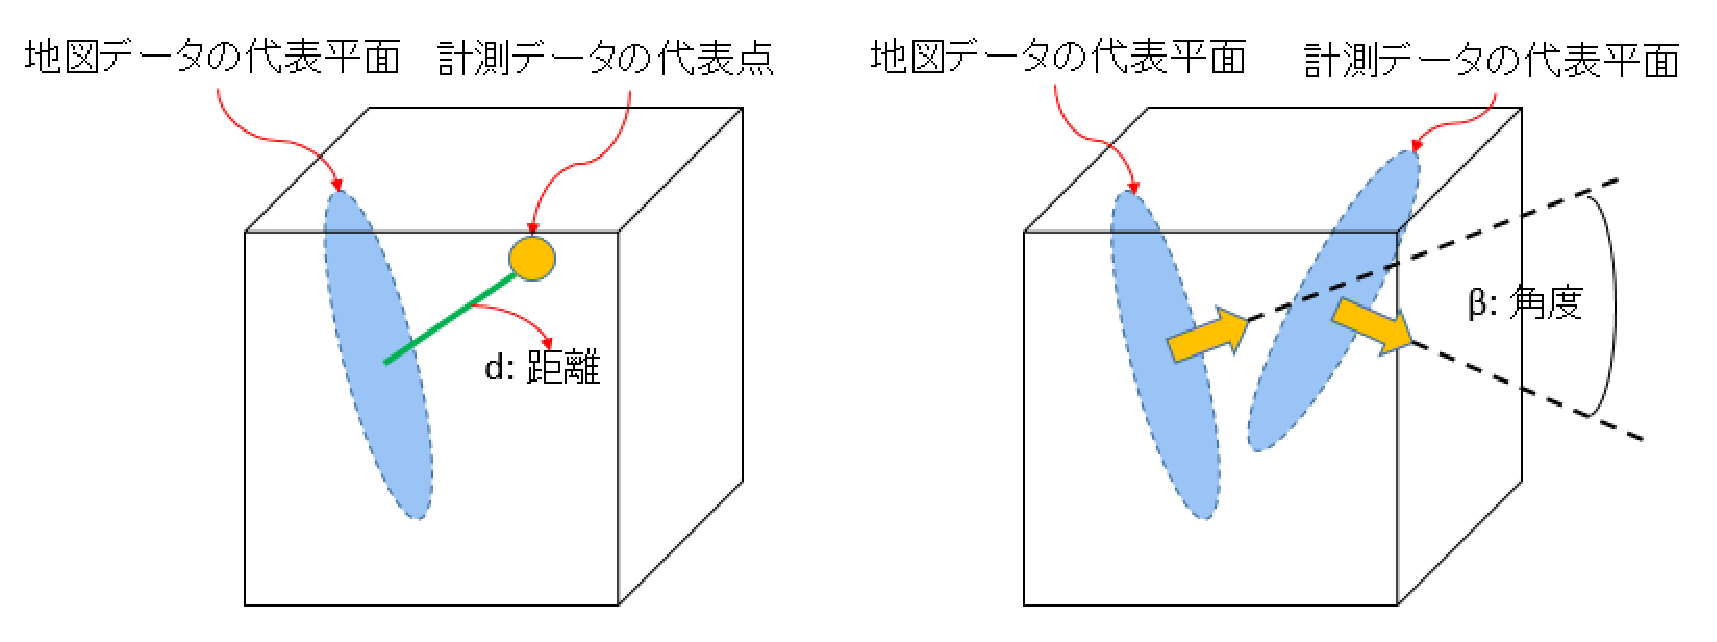
\includegraphics[height=60mm]{figure/尤度計算.eps}
   \caption{尤度計算}
   \label{尤度計算}
  \end{center}
\end{figure}
%
\vspace{15mm}
位置姿勢変換後の代表点が含まれる地図データ中の8個のオーバーラップ化されたボクセルm (m = 1~8)に対し,計測データの代表点と地図データの代表平面との距離$d_{ik->m}$を求める.正規分布に当てはめた代表点$\tilde{S}_{ik}$の距離評価値を$\alpha_{ik->m}$とする.地図データ中のボクセルmにおける代表平面の法線ベクトルを$N_{m}$とし,地図データ中のボクセルmの点群の平均位置を$\mu_{m}$とおくと,距離$d_{ik->m}$,$\alpha_{ik->m}$は以下のようになる.ここで$\sigma_{d}$は$d_{ik->m}$の分散値を表すパラメータである.図{\ref{尤度計算}}の左図に相当する計算である.\par

\begin{equation}
d_{ik->m} = |N_{mx}(S_{ikx}-\mu_{mx})+N_{my}(S_{iky}-\mu_{my})+N_{mz}(S_{ikz}-\mu_{mz})|
\end{equation}
\begin{equation}
\alpha_{ik->m} = \cfrac{1}{\sqrt{2\pi\sigma_{d}}}e^{-d^2_{ik->m}/\sigma_{d}^2}
\end{equation}

地図データのボクセルmと計測データのボクセルiの代表平面の相対角度の差を評価値$\beta_{i->m}$とする.$\beta_{i->m}$は以下のように求める.図{\ref{尤度計算}}から言うと右図に相当する計算である.\par
\begin{equation}
\beta_{i->m} = |N_{mx}\tilde{N}_{ix}+N_{my}\tilde{N}_{iy}+N_{mz}\tilde{N}_{iz}|
\end{equation}

代表点$S_{ik}$の総合評価値$\gamma_{ik}$は距離評価値を$\alpha_{ik->m}$と相対角度評価値$\beta_{i->m}$の積で求められるが,オーバーラップ化されている場合は以下のように各々の8つのボクセルで求めた総合評価値$\gamma_{ik}$の最大値として求める.\par

\begin{equation}
\gamma_{ik} = \max_{1 \leq m \leq 8}\alpha_{ik->m}\beta_{i->m}
\end{equation}

計測データボクセルiの評価値$\delta_{i}$はボクセルiにおける7つの代表点に対して評価値の和を計算する.最後に,計測データの全てのボクセル数に対して,評価値$\delta_{i}$の値を足すとパーティクルスコア$\lambda$が求められる.式は以下のようになる.\par

\begin{equation}
\delta_{i} = \sum_{k=1}^{7}\gamma_{ik}
\end{equation}

\begin{equation}
\lambda = \sum_{i=1}^{N}\delta_{i}
\end{equation}

まとめると,式(2.5)から(2.7)までは距離評価値を$\alpha_{ik->m}$と相対角度評価値$\beta_{i->m}$をもとめ,それらの値の積で,計測された代表点$\S_{ik}$の総合評価値$\gamma_{ik}$を計算している.これはそれぞれの評価値を条件付き確率とみなし,代表点ごとの尤度を計算したものである.式(2.9)と式(2.10)は式(2.5)から(2.7)の尤度計算で求めた各代表点の評価値を全代表点及び全ボクセルの数分足したものである.最後に求められたパーティクルスコア$\lambda$が最終的な重さとなる.


\newpage
パーティクルフィルタを用いて収束する過程の例を図{\ref{収束過程の例}}に表す.図2.9で,緑はパーティクルの位置,青は3次元地図,赤は計測した3次元点,黒は最も尤度が高いパーティクルの位置である.
\vspace{10mm}
\begin{figure}[htbp]
  \begin{center}
   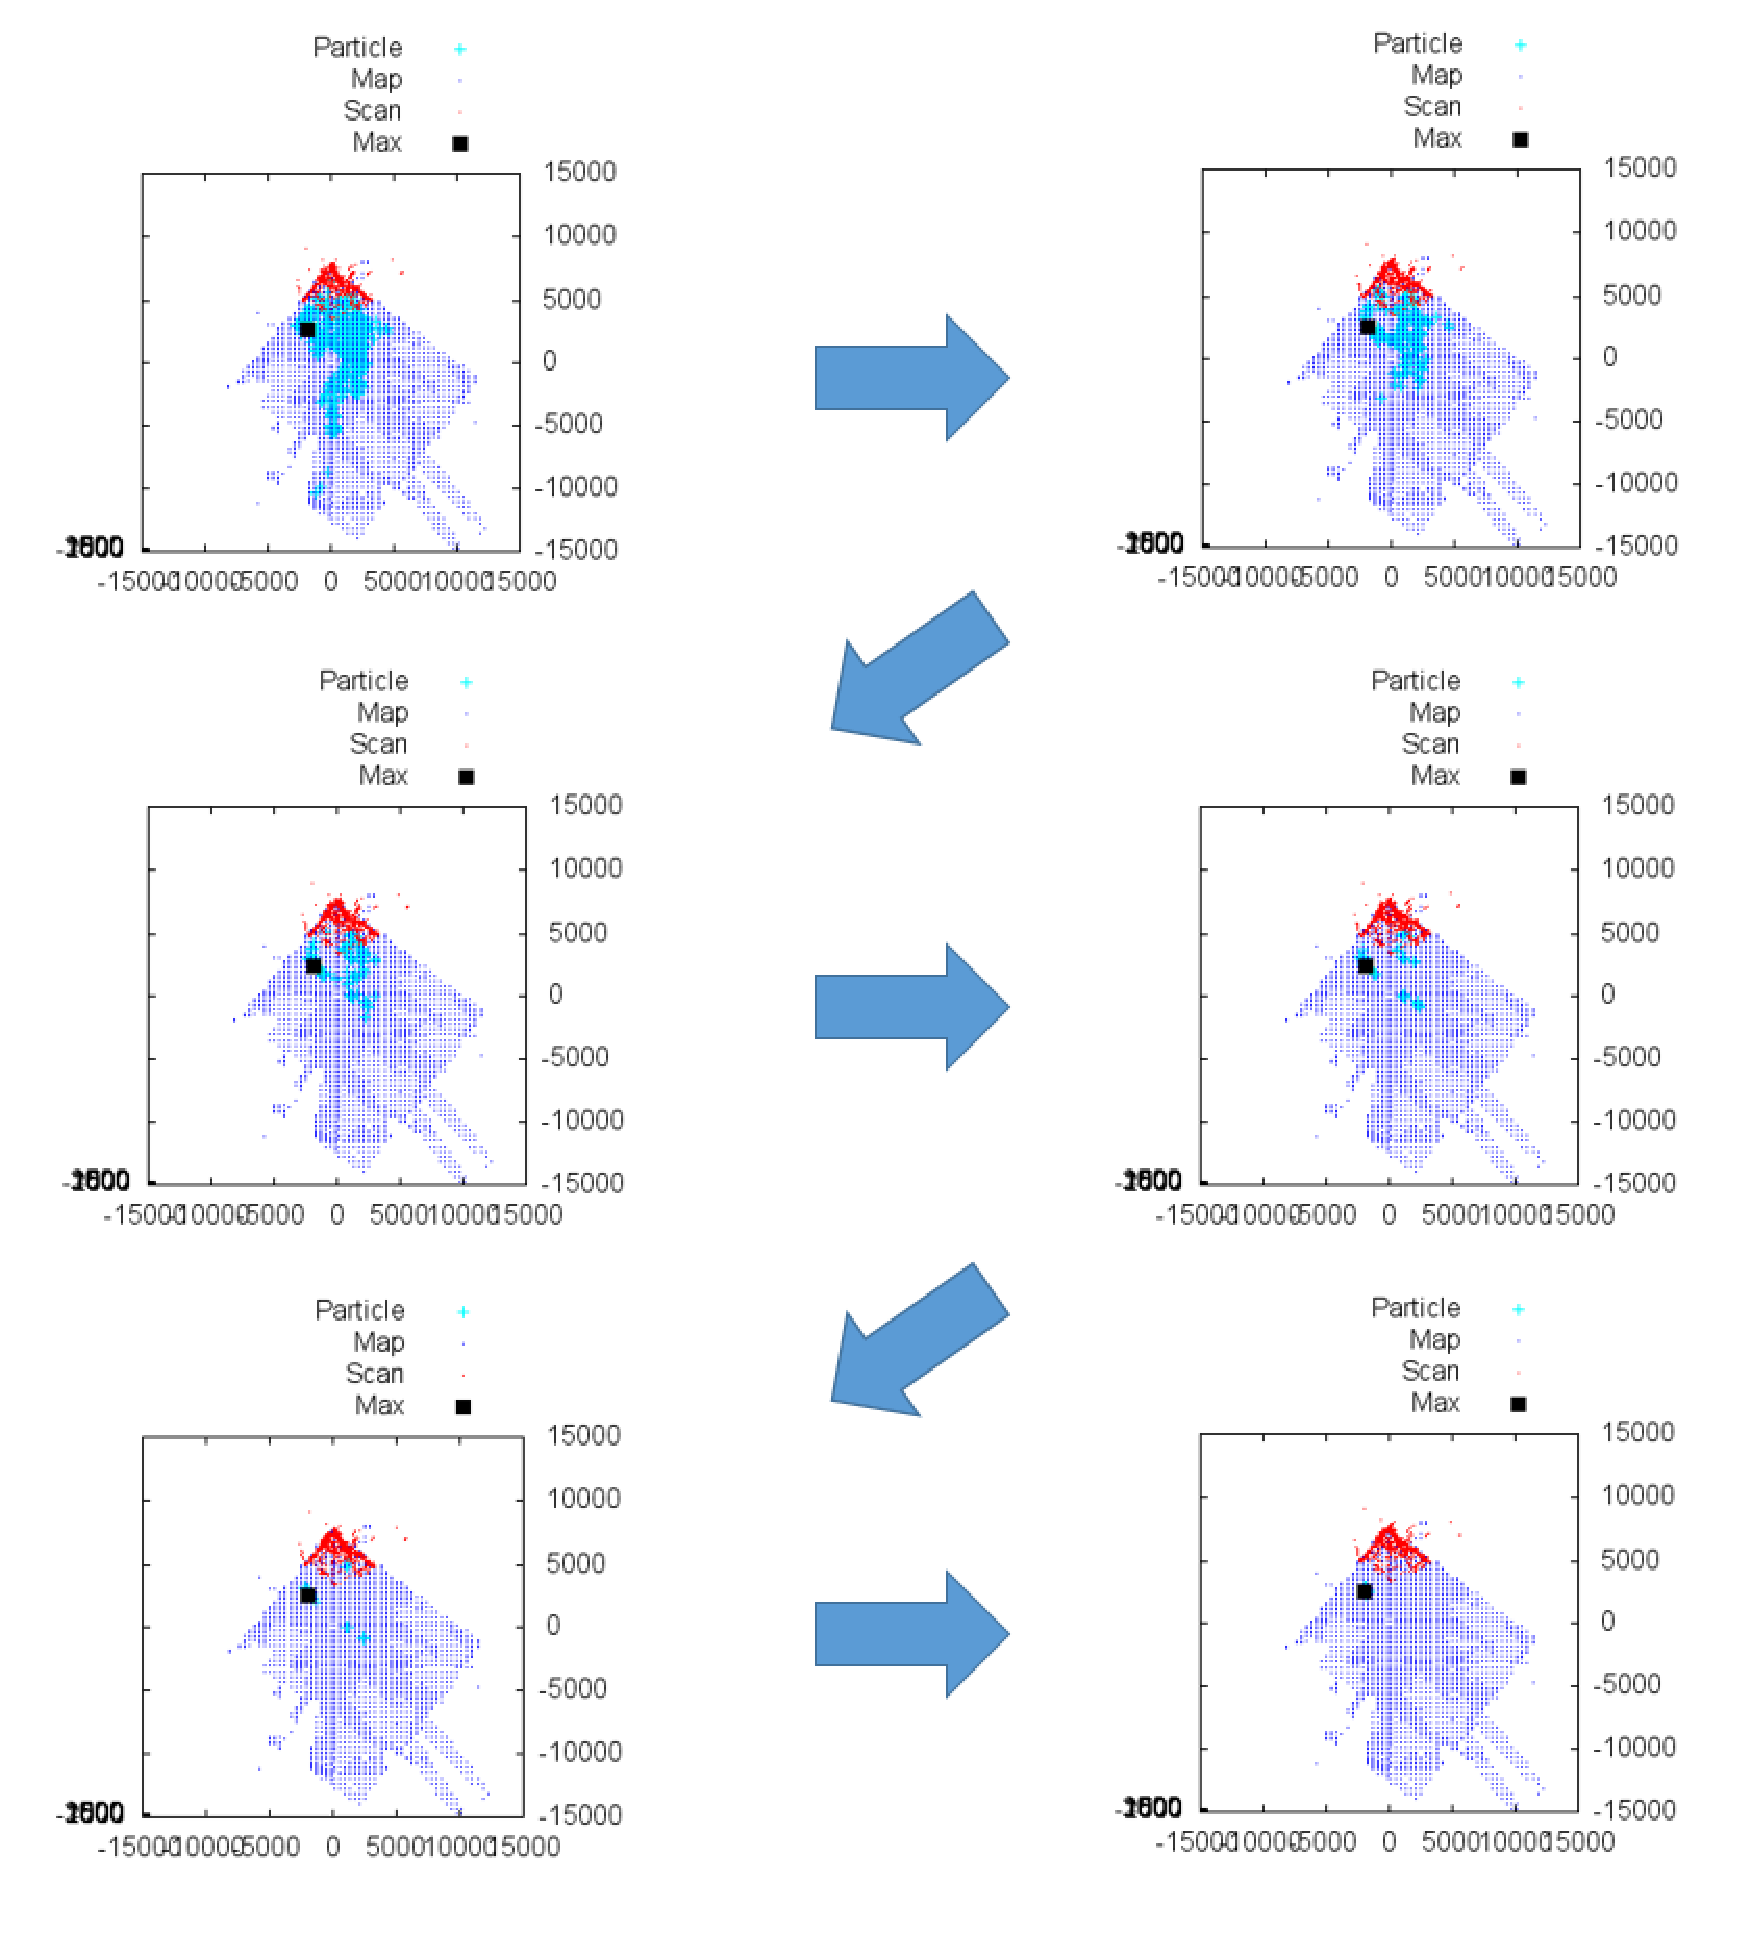
\includegraphics[height=150mm]{figure/収束過程の例.eps}
   \caption{収束過程の例}
   \label{収束過程の例}
  \end{center}
\end{figure}
%
\newpage
%
%---------------------------------------------------------------------------------------------------
%===================================================================================================
% システム設計
%===================================================================================================
\chapter{ステレオカメラを用いた位置同定}
本章では,位置同定実験を行う際用いられた装置,データ,及びデータの取得法について述べる.

%---------------------------------------------------------------------------------------------------
\section{概要}
本研究の目的は,ステレオカメラを用いた屋内・屋外位置同定である.そこで,ここでは位置同定実験を行う際用いられた装置や,データ,データ取得法について述べる.
本章の流れについて説明すると,まずは提供されたステレオカメラについて述べる.ステレオカメラデータ取得部のシステム構成,キャリブレーション方法,ステレオカメラ画像の特徴などについて説明する.また,今回実験を行う際,用いられたステレオカメラ搭載の実験用台車について述べる.最後に環境地図の生成方法と台車の位置計測法について述べる.なお,本研究では地図データや計測データはすべてPTX形式で表現,保存されている..
\newpage
%---------------------------------------------------------------------------------------------------
\section{ステレオカメラ}

\subsection{ステレオカメラデータ取得部のシステム構成}
ステレオカメラデータ取得部のシステム構成説明の前に,ステレオカメラについて述べる.本研究で用いたステレオカメラはセンサーフォーマット1/1.8インチで有効画像数が1280*640である.レンズの水平視野角89°,焦点距離3.5mm,取得レート15fps,それに,絞りF4.0である物となる.ステレオカメラ2つの間は300mmに置いて撮ったデータはMRPT改造 Rawlog-Grabberというキャッチャーソフトにより左右のJPG画像ができる.OpenCV(C++)視差画像生成ソフトを用いて距離画像(Depth画像)とカラー画像(RGB画像)を生成する.このときキャリブレーションソフトによるステレオカメラの歪・平行化補正が行われる.最後に,MRPT改造 Kinect-3D-SLAMというVisual Odometoryソフトを用いることにより,PointCloudの3次元表示ができる.今回用いたステレオカメラを図{\ref{ステレオカメラ}}に表す.また,図{\ref{システム構成}}にステレオカメラデータ取得部のシステム構成の流れを表す.

\vspace{5mm}
\begin{figure}[htbp]
  \begin{center}
   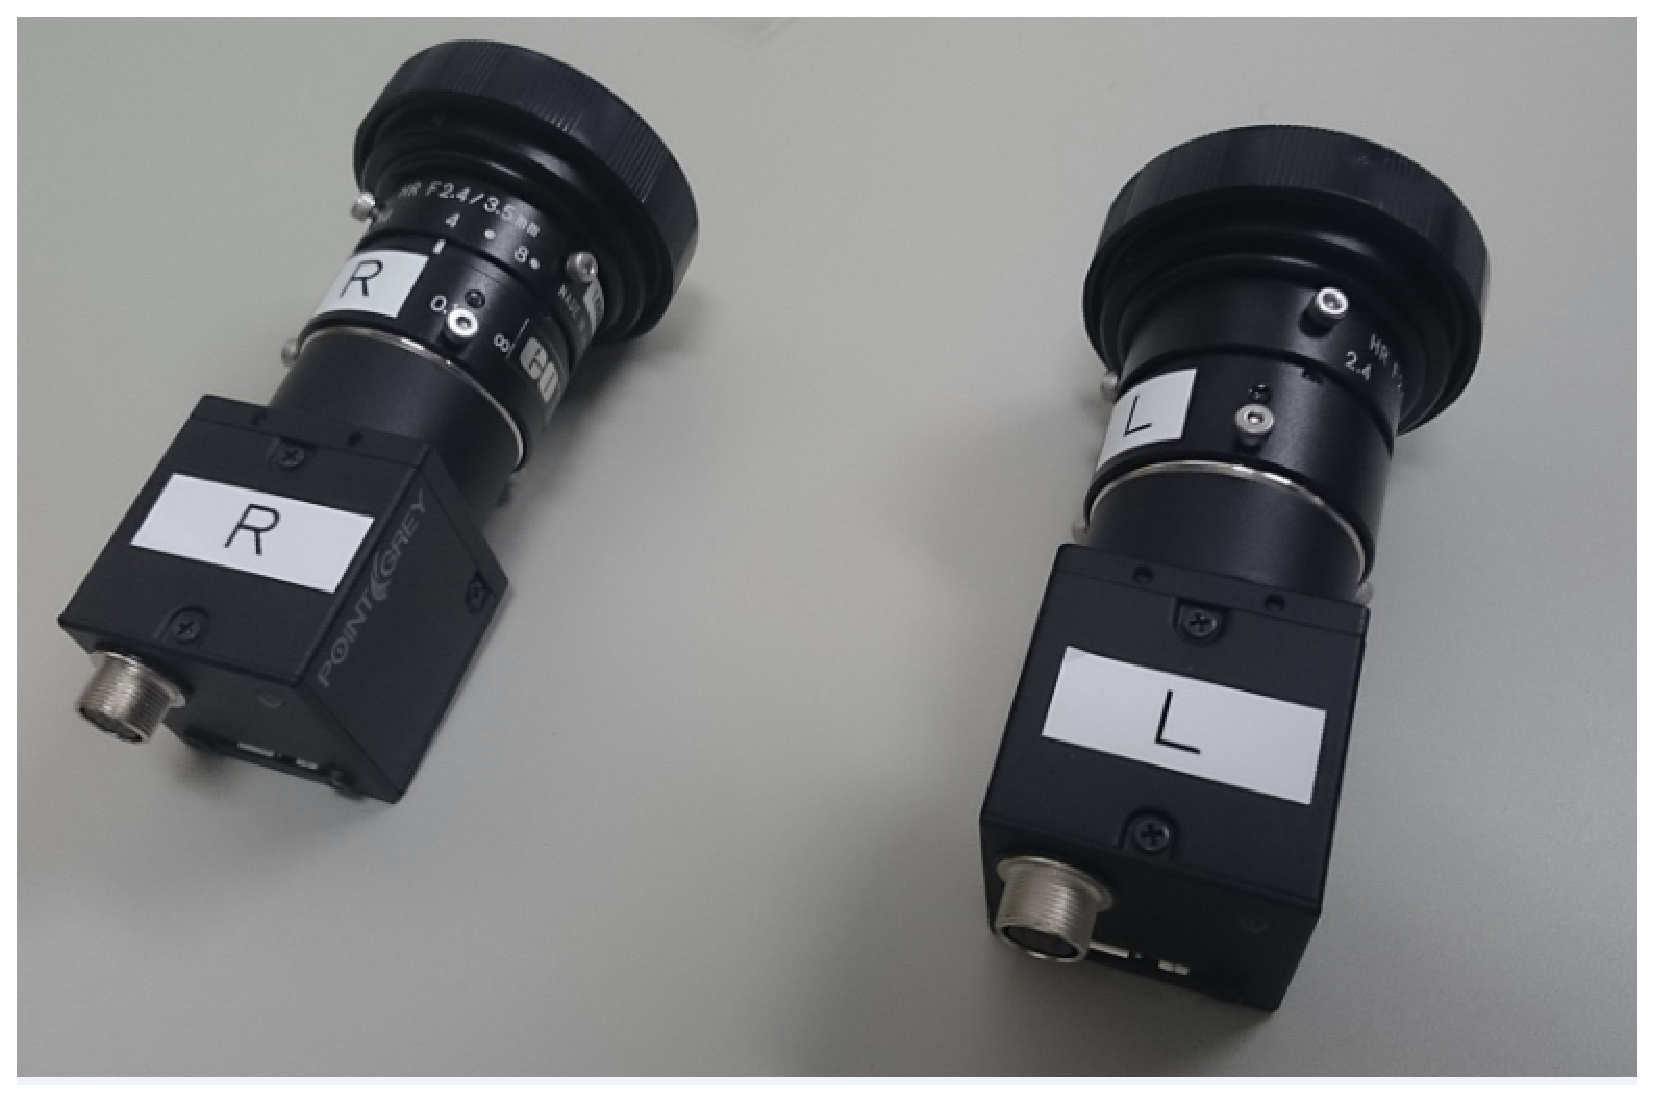
\includegraphics[height=60mm]{figure/ステレオカメラ.eps}
   \caption{ステレオカメラ}
   \label{ステレオカメラ}
  \end{center}
\end{figure}

\newpage

\vspace{5mm}
\begin{figure}[htbp]
  \begin{center}
   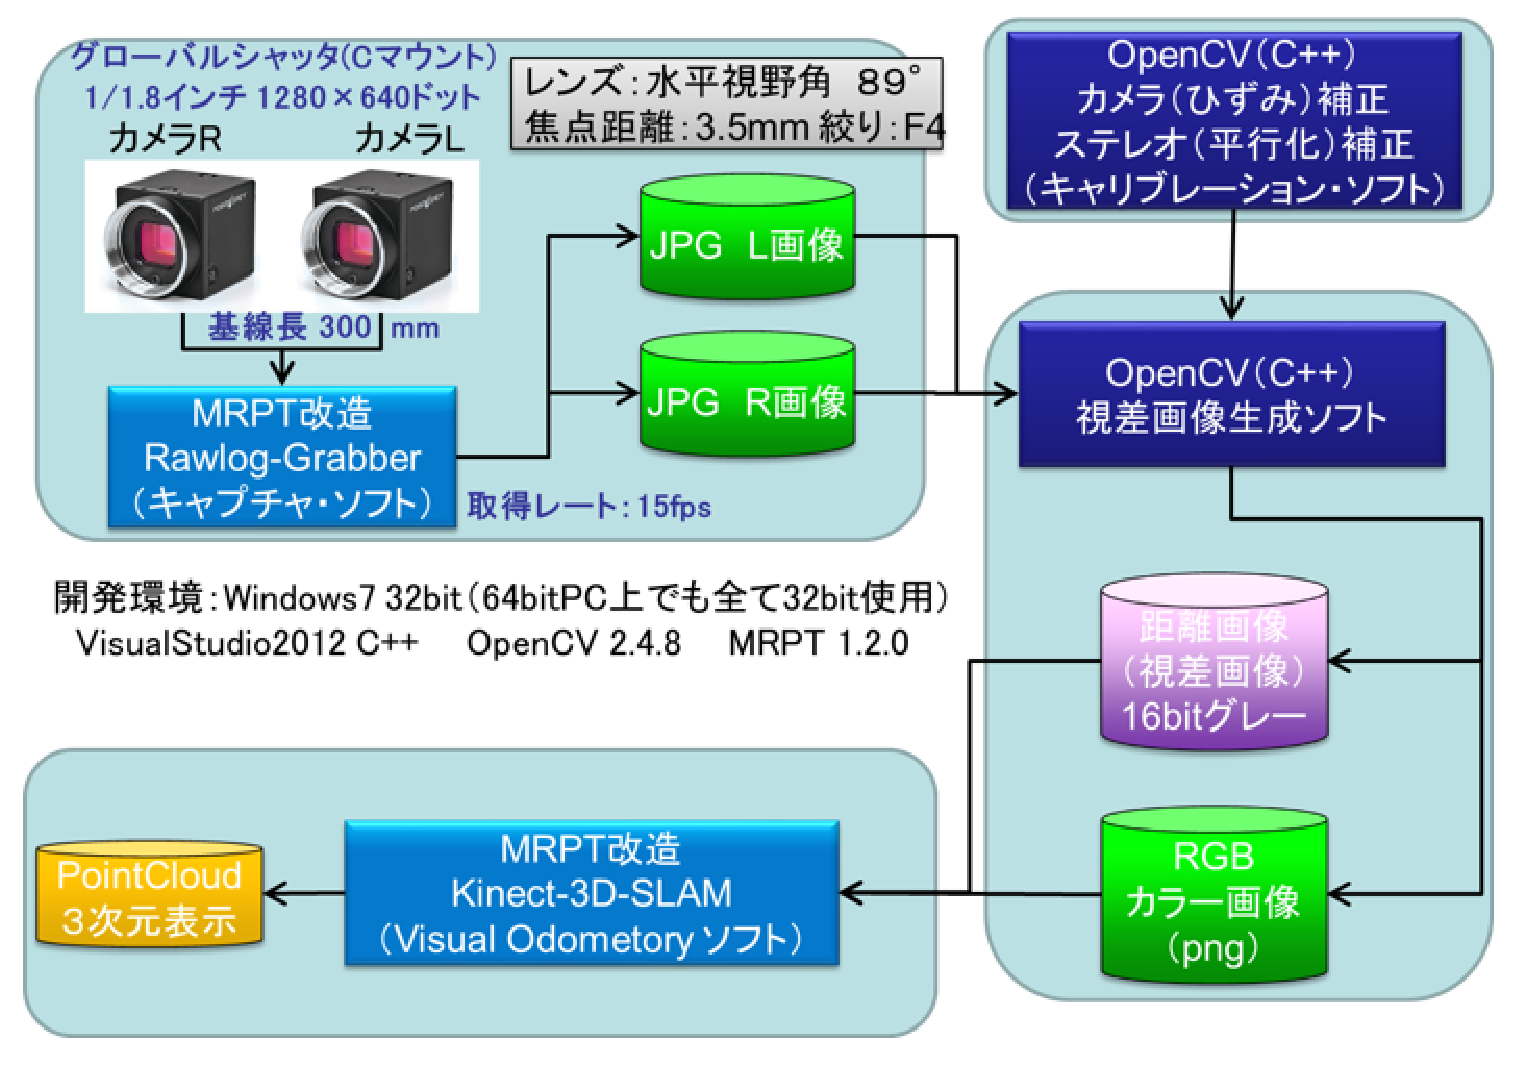
\includegraphics[height=80mm]{figure/システム構成.eps}
   \caption{システム構成}
   \label{システム構成}
  \end{center}
\end{figure}

\subsection{キャリブレーション}
前述した通り,ステレオカメラの歪・平行化補正を行うためにはキャリブレーションを行う必要がある.そこで,キャリブレーションの手順について述べる.
キャリブレーションする前にカメラ準備が要る.カメラ準備の手順は下のようになる.

\begin{enumerate}
 \item ステレオカメラにレンズを付ける.
 \item ステレオカメラをプレートにつけ,三脚に建てる.
 \begin{itemize}
      \item キャリブレーションする際は,ステレオカメラを三脚につける必要があるため,プレートが要る.プレートのイメージを図3.3に表す.また,図{\ref{プレート}}に実際のプレート付きのステレオカメラを表す.
 \end{itemize}

\begin{figure}[htbp]
  \begin{center}
   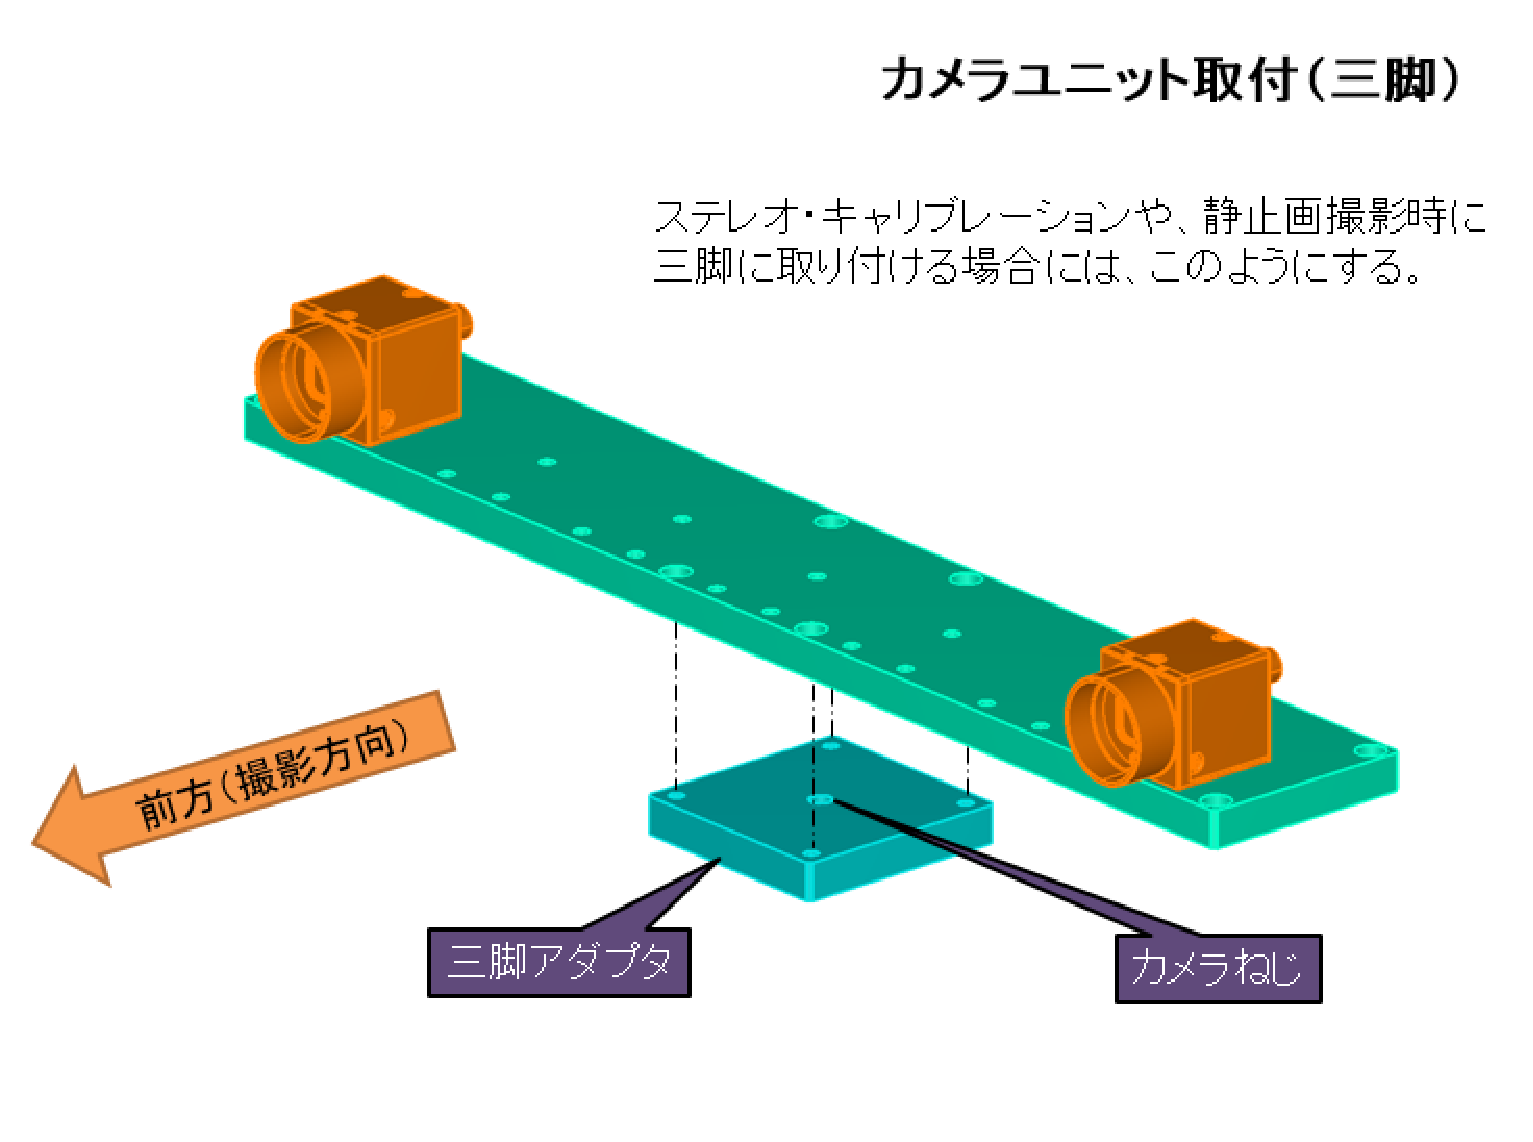
\includegraphics[height=80mm]{figure/プレートイメージ.eps}
   \caption{プレートイメージ}
   \label{プレートイメージ}
  \end{center}
\end{figure}
\begin{figure}[htbp]
  \begin{center}
   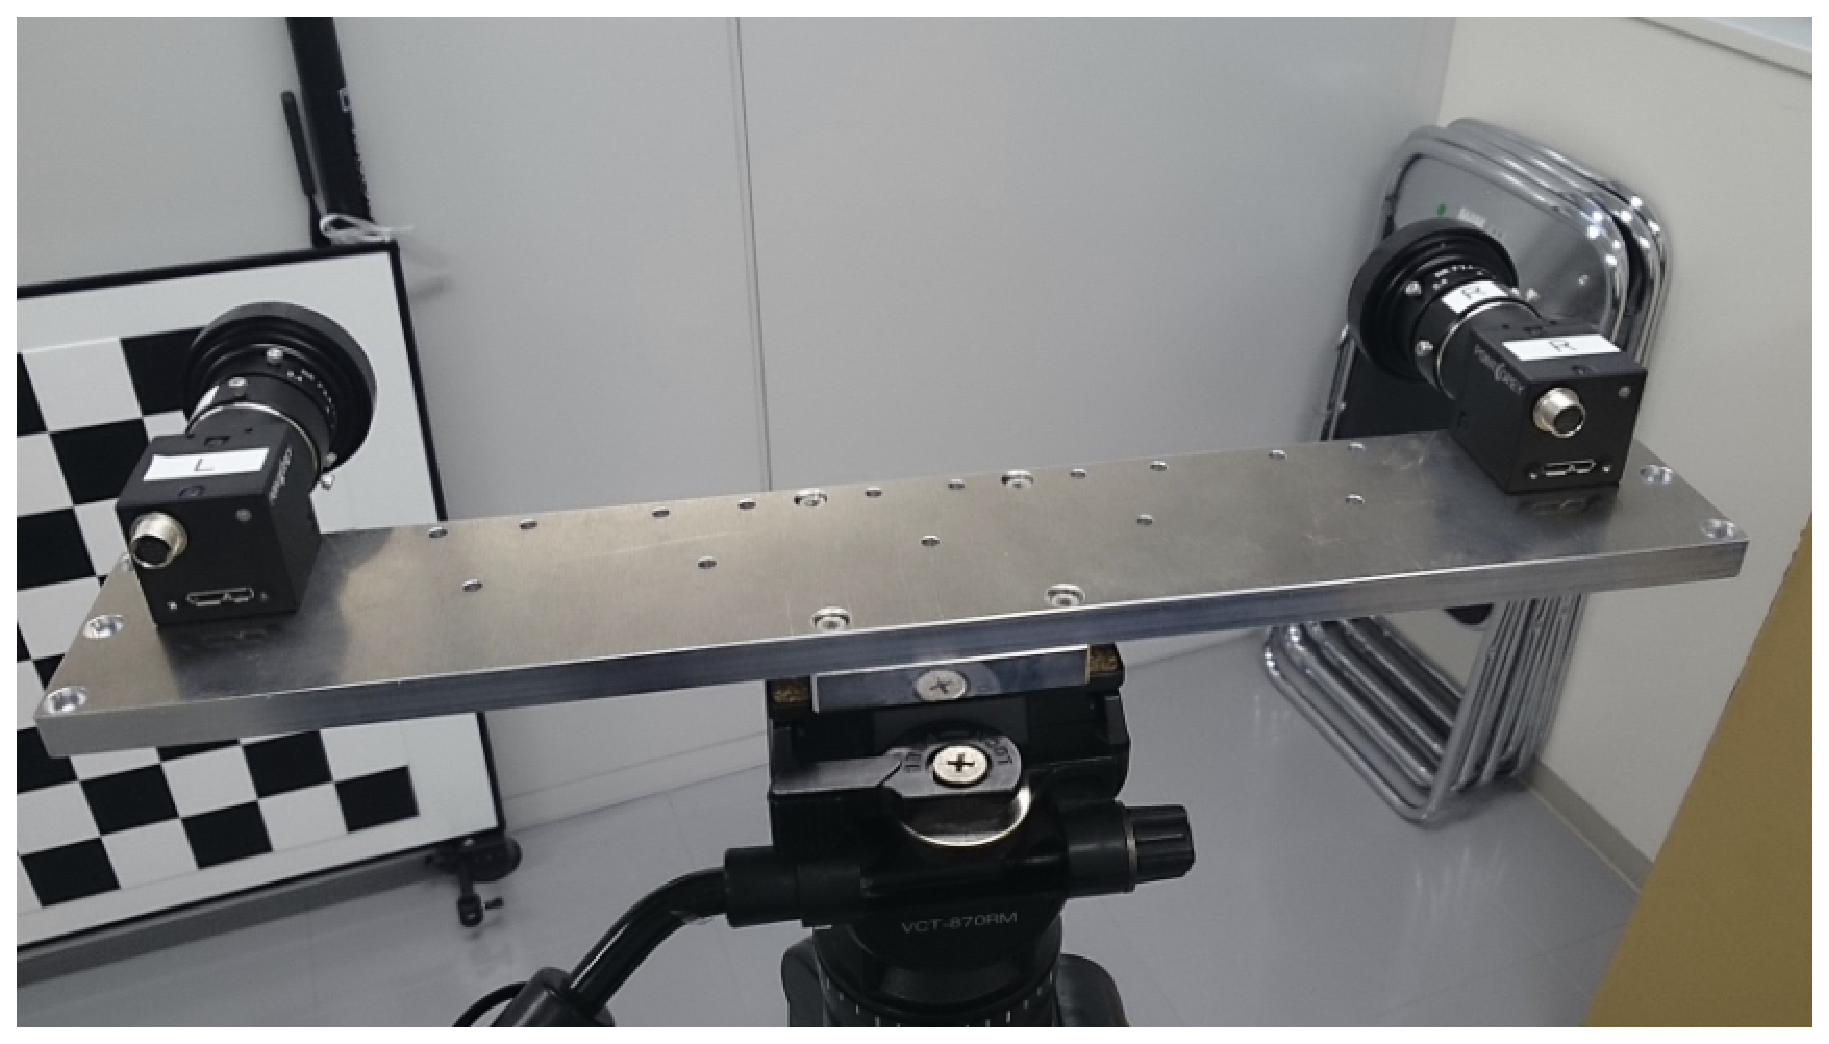
\includegraphics[height=80mm]{figure/プレート.eps}
   \caption{プレート}
   \label{プレート}
  \end{center}
\end{figure}
 \item USB3.0ケーブルをカメラとPCに繋げる.
  \begin{itemize}
      \item このステレオカメラはデータをUSB3.0ケーブルを用いてPCに通す.図3.5にキャリブレーション際の設置イメージを表す.
\begin{figure}[htbp]
  \begin{center}
   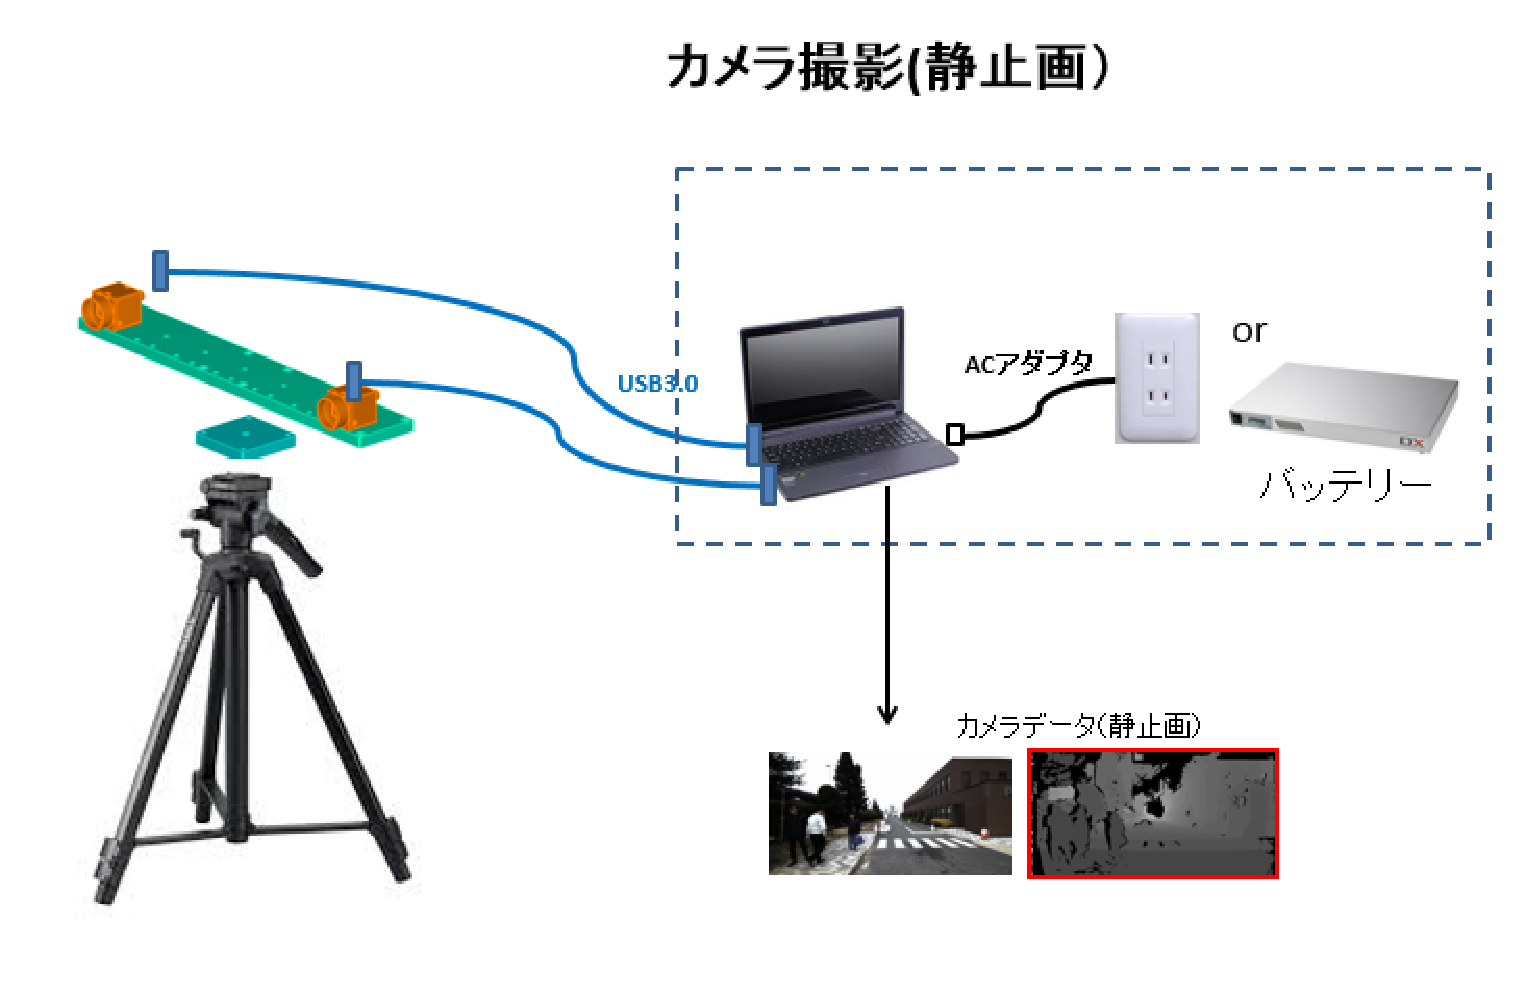
\includegraphics[height=80mm]{figure/設置イメージ.eps}
   \caption{設置イメージ}
   \label{設置イメージ}
  \end{center}
\end{figure}
 \end{itemize}
 \item キャリブレーション撮影ツールを起動し,ステレオカメラの左右確認及びフォーカス調整をする.
\end{enumerate}

ここまでが,カメラ準備の手順となり,キャリブレーションの手順は下のようになる.

\begin{enumerate}
\item キャリブレーションボードを設置して,キャリブレーション撮影ツールを起動する.
\begin{itemize}
\item キャリブレーションボードを図{\ref{キャリブレーションボード}}に,構成を以下に示す.
\item 小アクリル板\\
  各90mm x 90mm, 厚み2.0mm、2色(白黒) 各44枚
\item 大アクリル板\\
  A0サイズ(841mm x 1189mm)\\
  縦8枚 x 横11枚= 合計88枚(720mm x 990mm)の小アクリル板を、大きなアクリル板上の\\
  中央に白黒交互に貼り合わせする.
\item 補強として、枠が小アクリル板と重ならないようにするため,外側に枠を取り付けする.
\begin{figure}[htbp]
  \begin{center}
   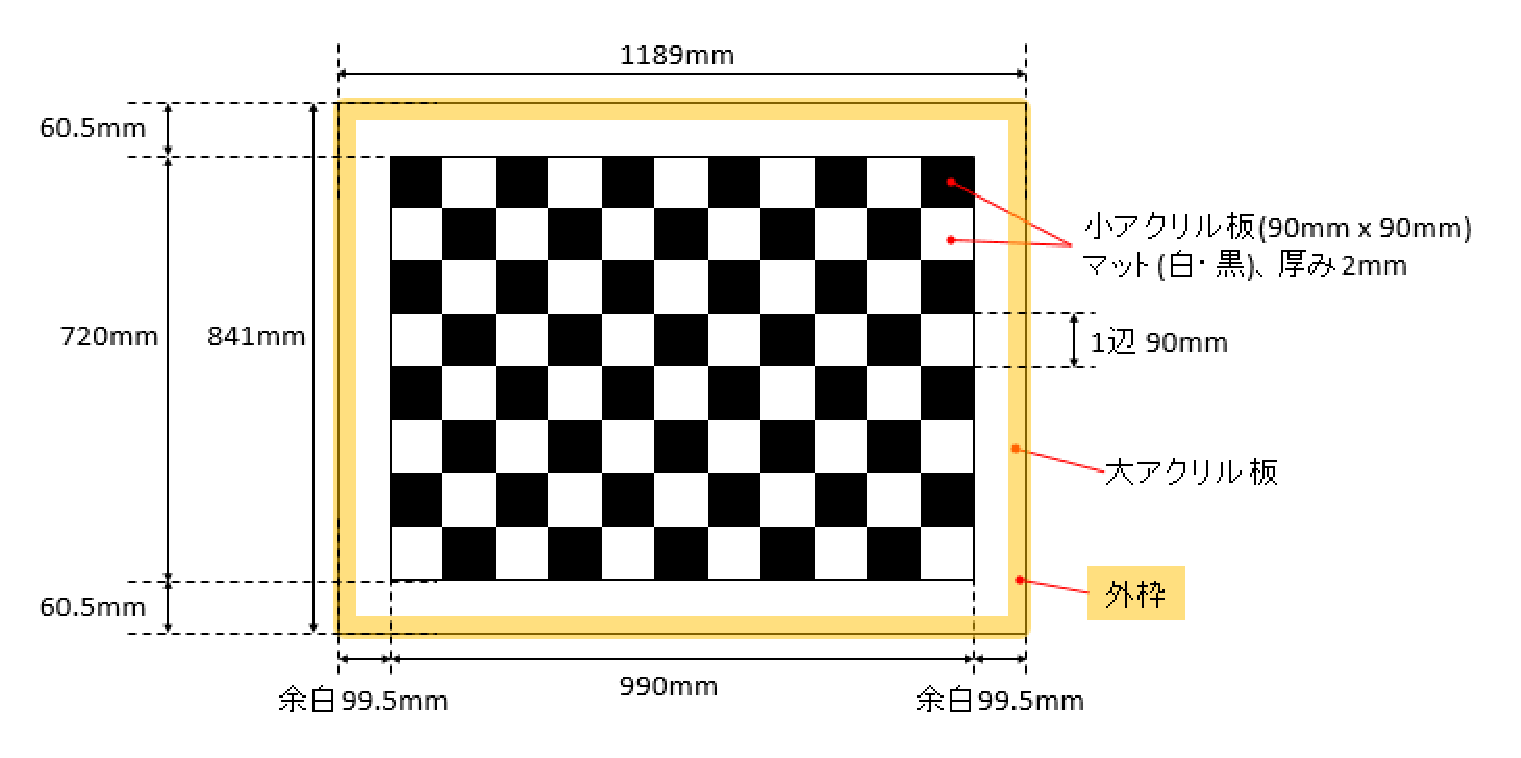
\includegraphics[height=80mm]{figure/キャリブレーションボード.eps}
   \caption{キャリブレーションボード}
   \label{キャリブレーションボード}
  \end{center}
\end{figure}
\end{itemize}

\vspace{15mm}
\item ボードの上(三脚高さ:1.5m,ボードの高さ:1m)\\
->左(カメラを左に傾け),左(右に傾け),中央,右(左に傾け),右(右に傾け)\\

ボードの中央\\
->左(ボードからの距離:50cm),左(ボードからの距離:100cm),中央(ボードからの距離:50cm)\\
中央(ボードからの距離:100cm),右(ボードからの距離:50cm), 右(ボードからの距離:100cm)\\

ボードの下(三脚高さ:0.5m,ボードの高さ:1.7m)\\
->左(左に傾け),左(右に傾け),中央,右(左に傾け),右(右に傾け)\\

暗室で照明が安定なところで総16パターン撮影を行う.図3.7,図3.8にキャリブレーション撮影例を表す.

\begin{figure}[htbp]
  \begin{center}
   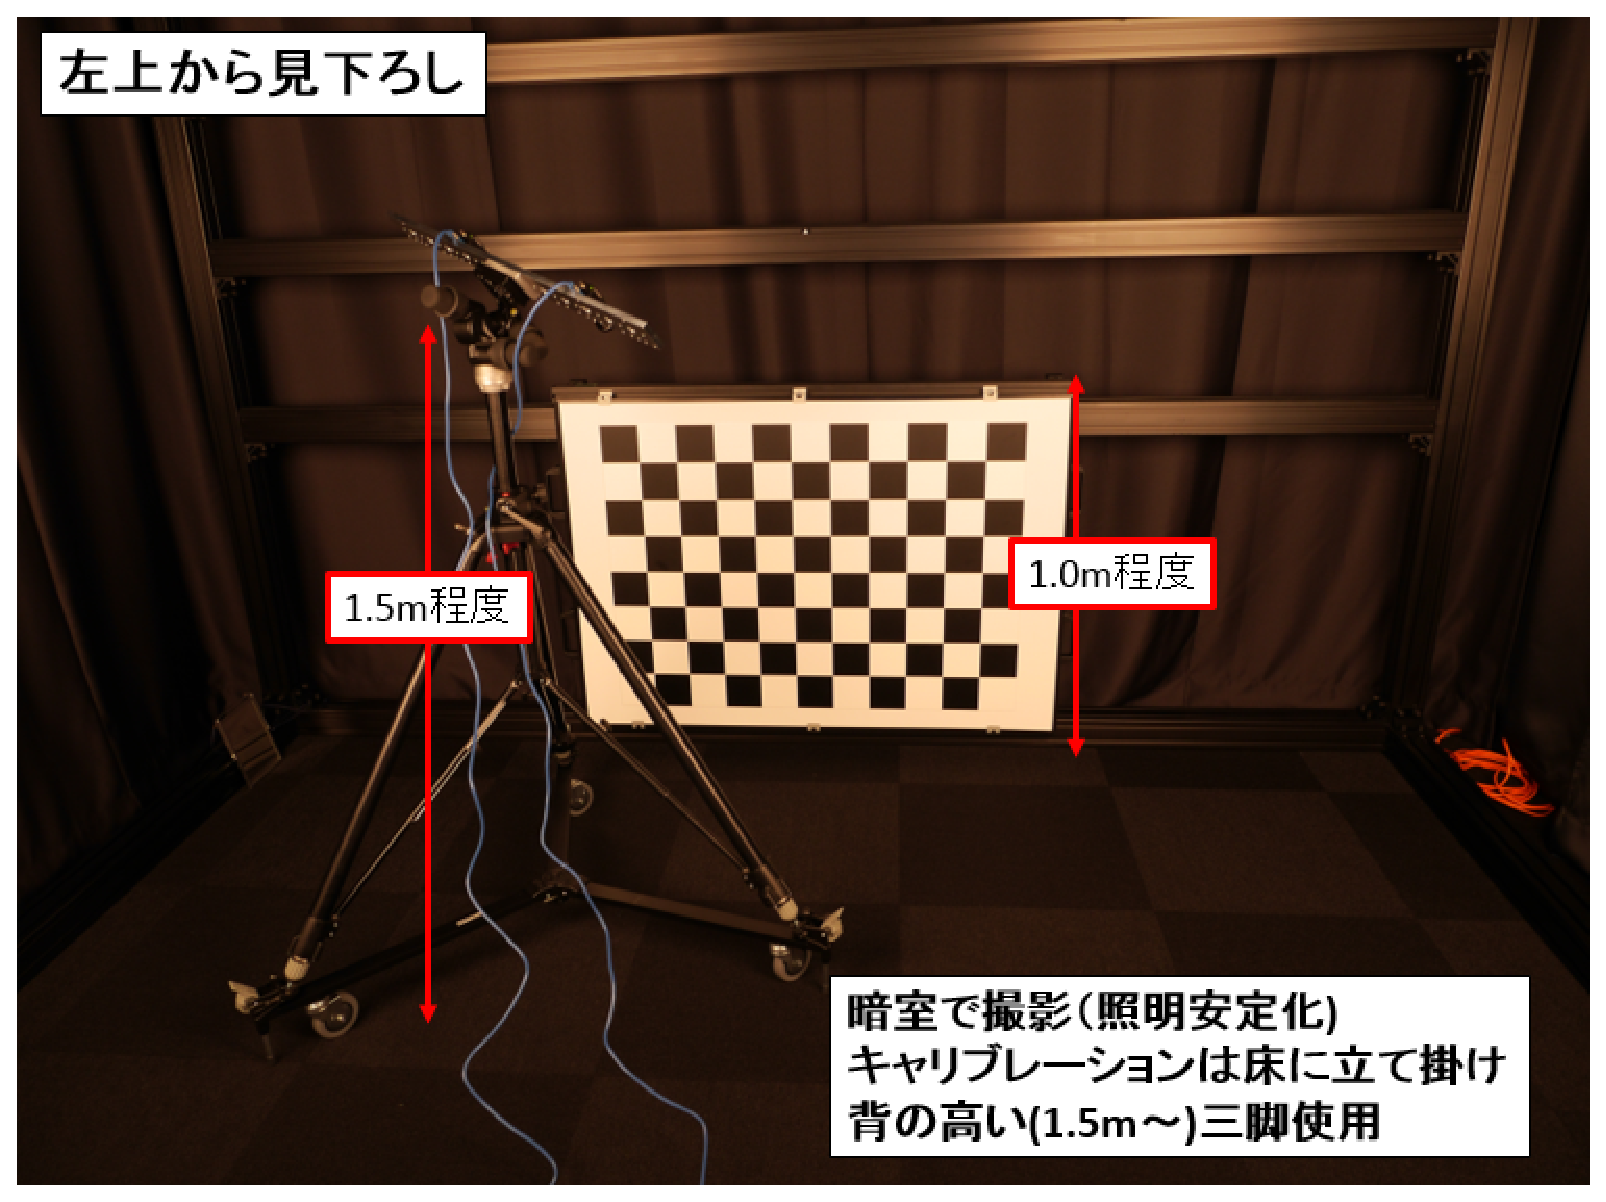
\includegraphics[height=80mm]{figure/caribration1.eps}
   \caption{キャリブレーション撮影例1}
   \label{caribration1}
  \end{center}
\end{figure}

\begin{figure}[htbp]
  \begin{center}
   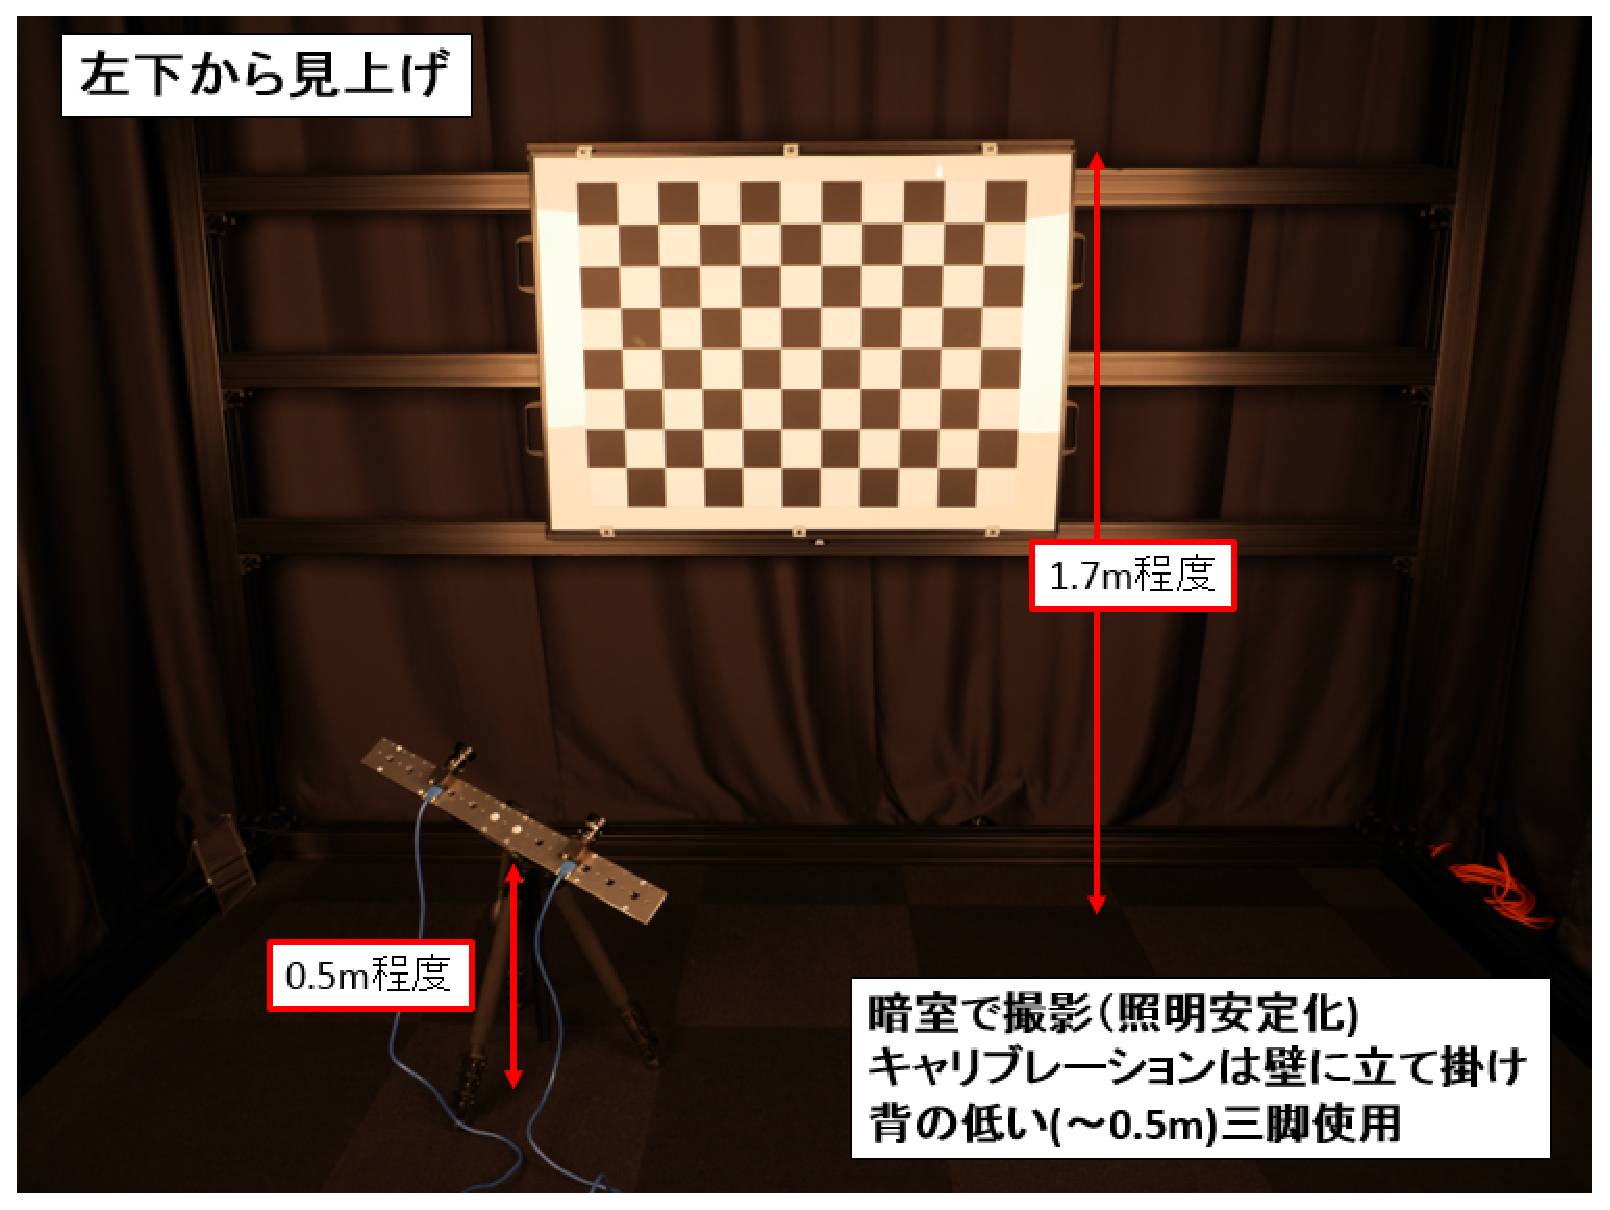
\includegraphics[height=80mm]{figure/caribration2.eps}
   \caption{キャリブレーション撮影例2}
   \label{caribration2}
  \end{center}
\end{figure}

\item キャリブレーション実行ツールを起動する.

\end{enumerate}
\newpage

\subsection{ステレオ画像の特徴}
ステレオ画像とは, 景色や物などを2つの視点から撮った画像を左右に並べたものである.2つの視点はそれぞれ右目と左目で見たように水平方向にお互いに少し離れている.2つの視点から各々見られる画像は少しズレがあるが,それを視差という.左右の視点間の距離と対応点の視差から,奥行きが計算できる.

ステレオカメラから得られる距離画像(ステレオ画像)と,RGB-Dカメラから得られる距離画像(RGB-D画像)を図3.9,図3.10に表す.各々の図はMeshLabを用いてPTX化されたデータを表示したもので,ステレオ画像のデータを安定に撮れるようにするため,壁にテクスチャーを貼った状態である.\\

\begin{figure}[ht]
  \begin{center}
   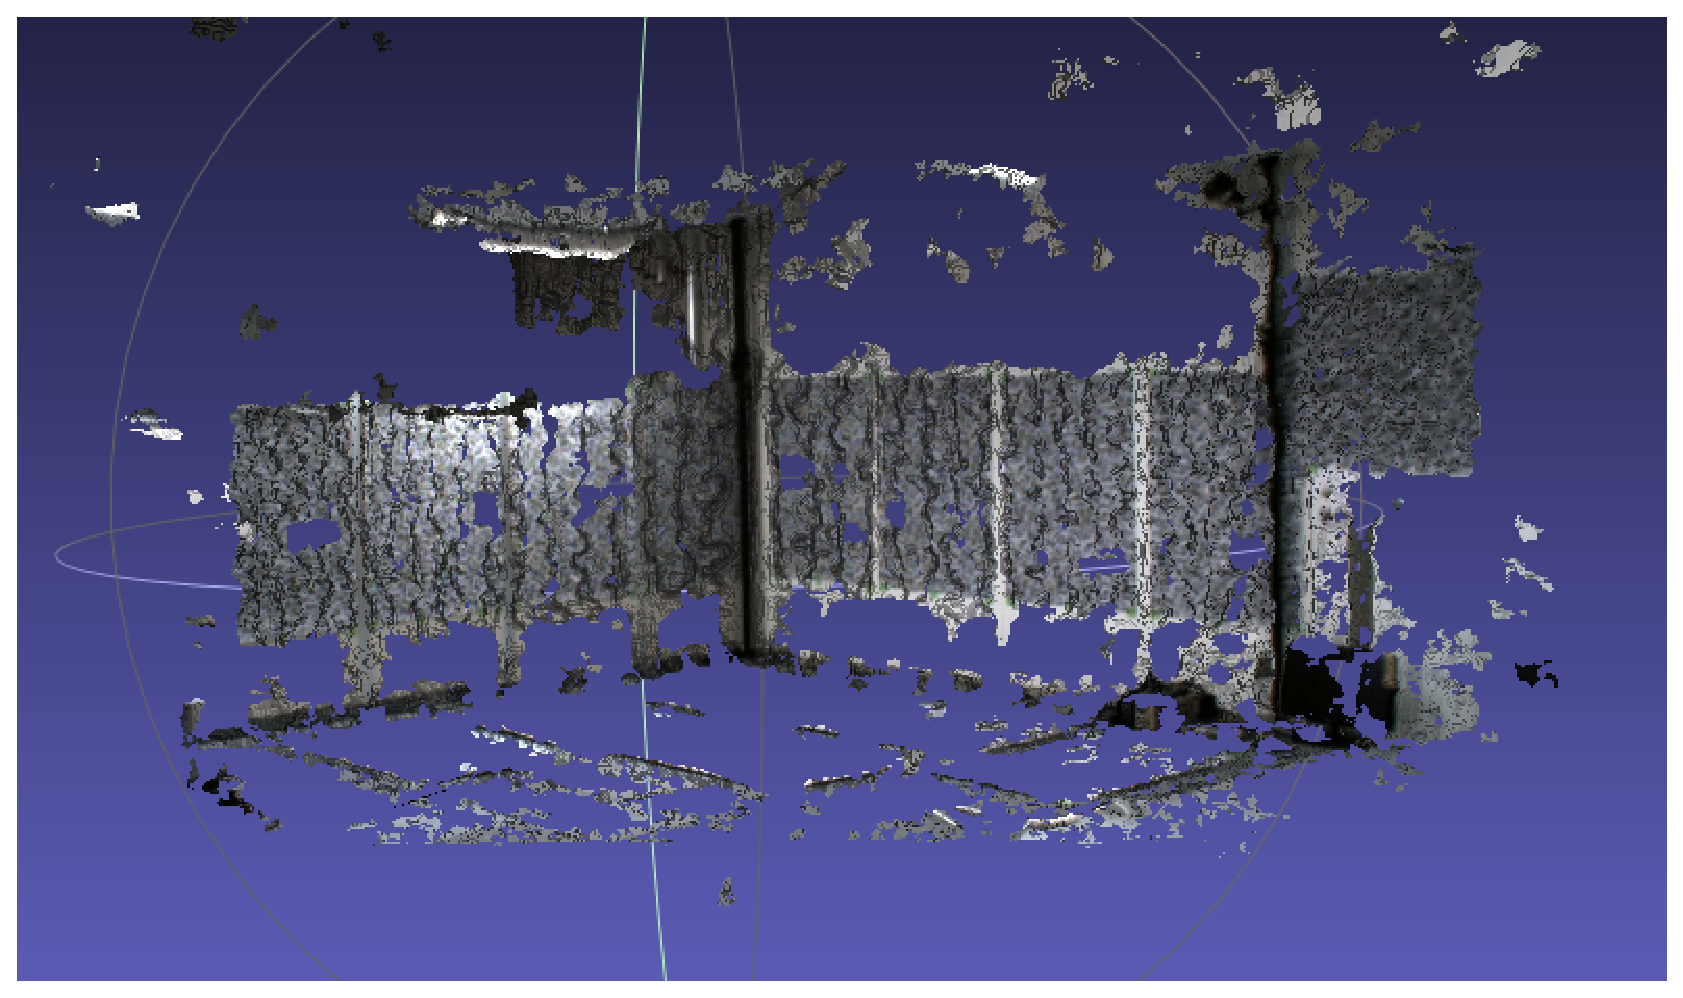
\includegraphics[height=50mm]{figure/ステレオ画像.eps}
   \caption{ステレオ画像}
   \label{ステレオ画像}
  \end{center}
\end{figure}

\begin{figure}[h]
  \begin{center}
   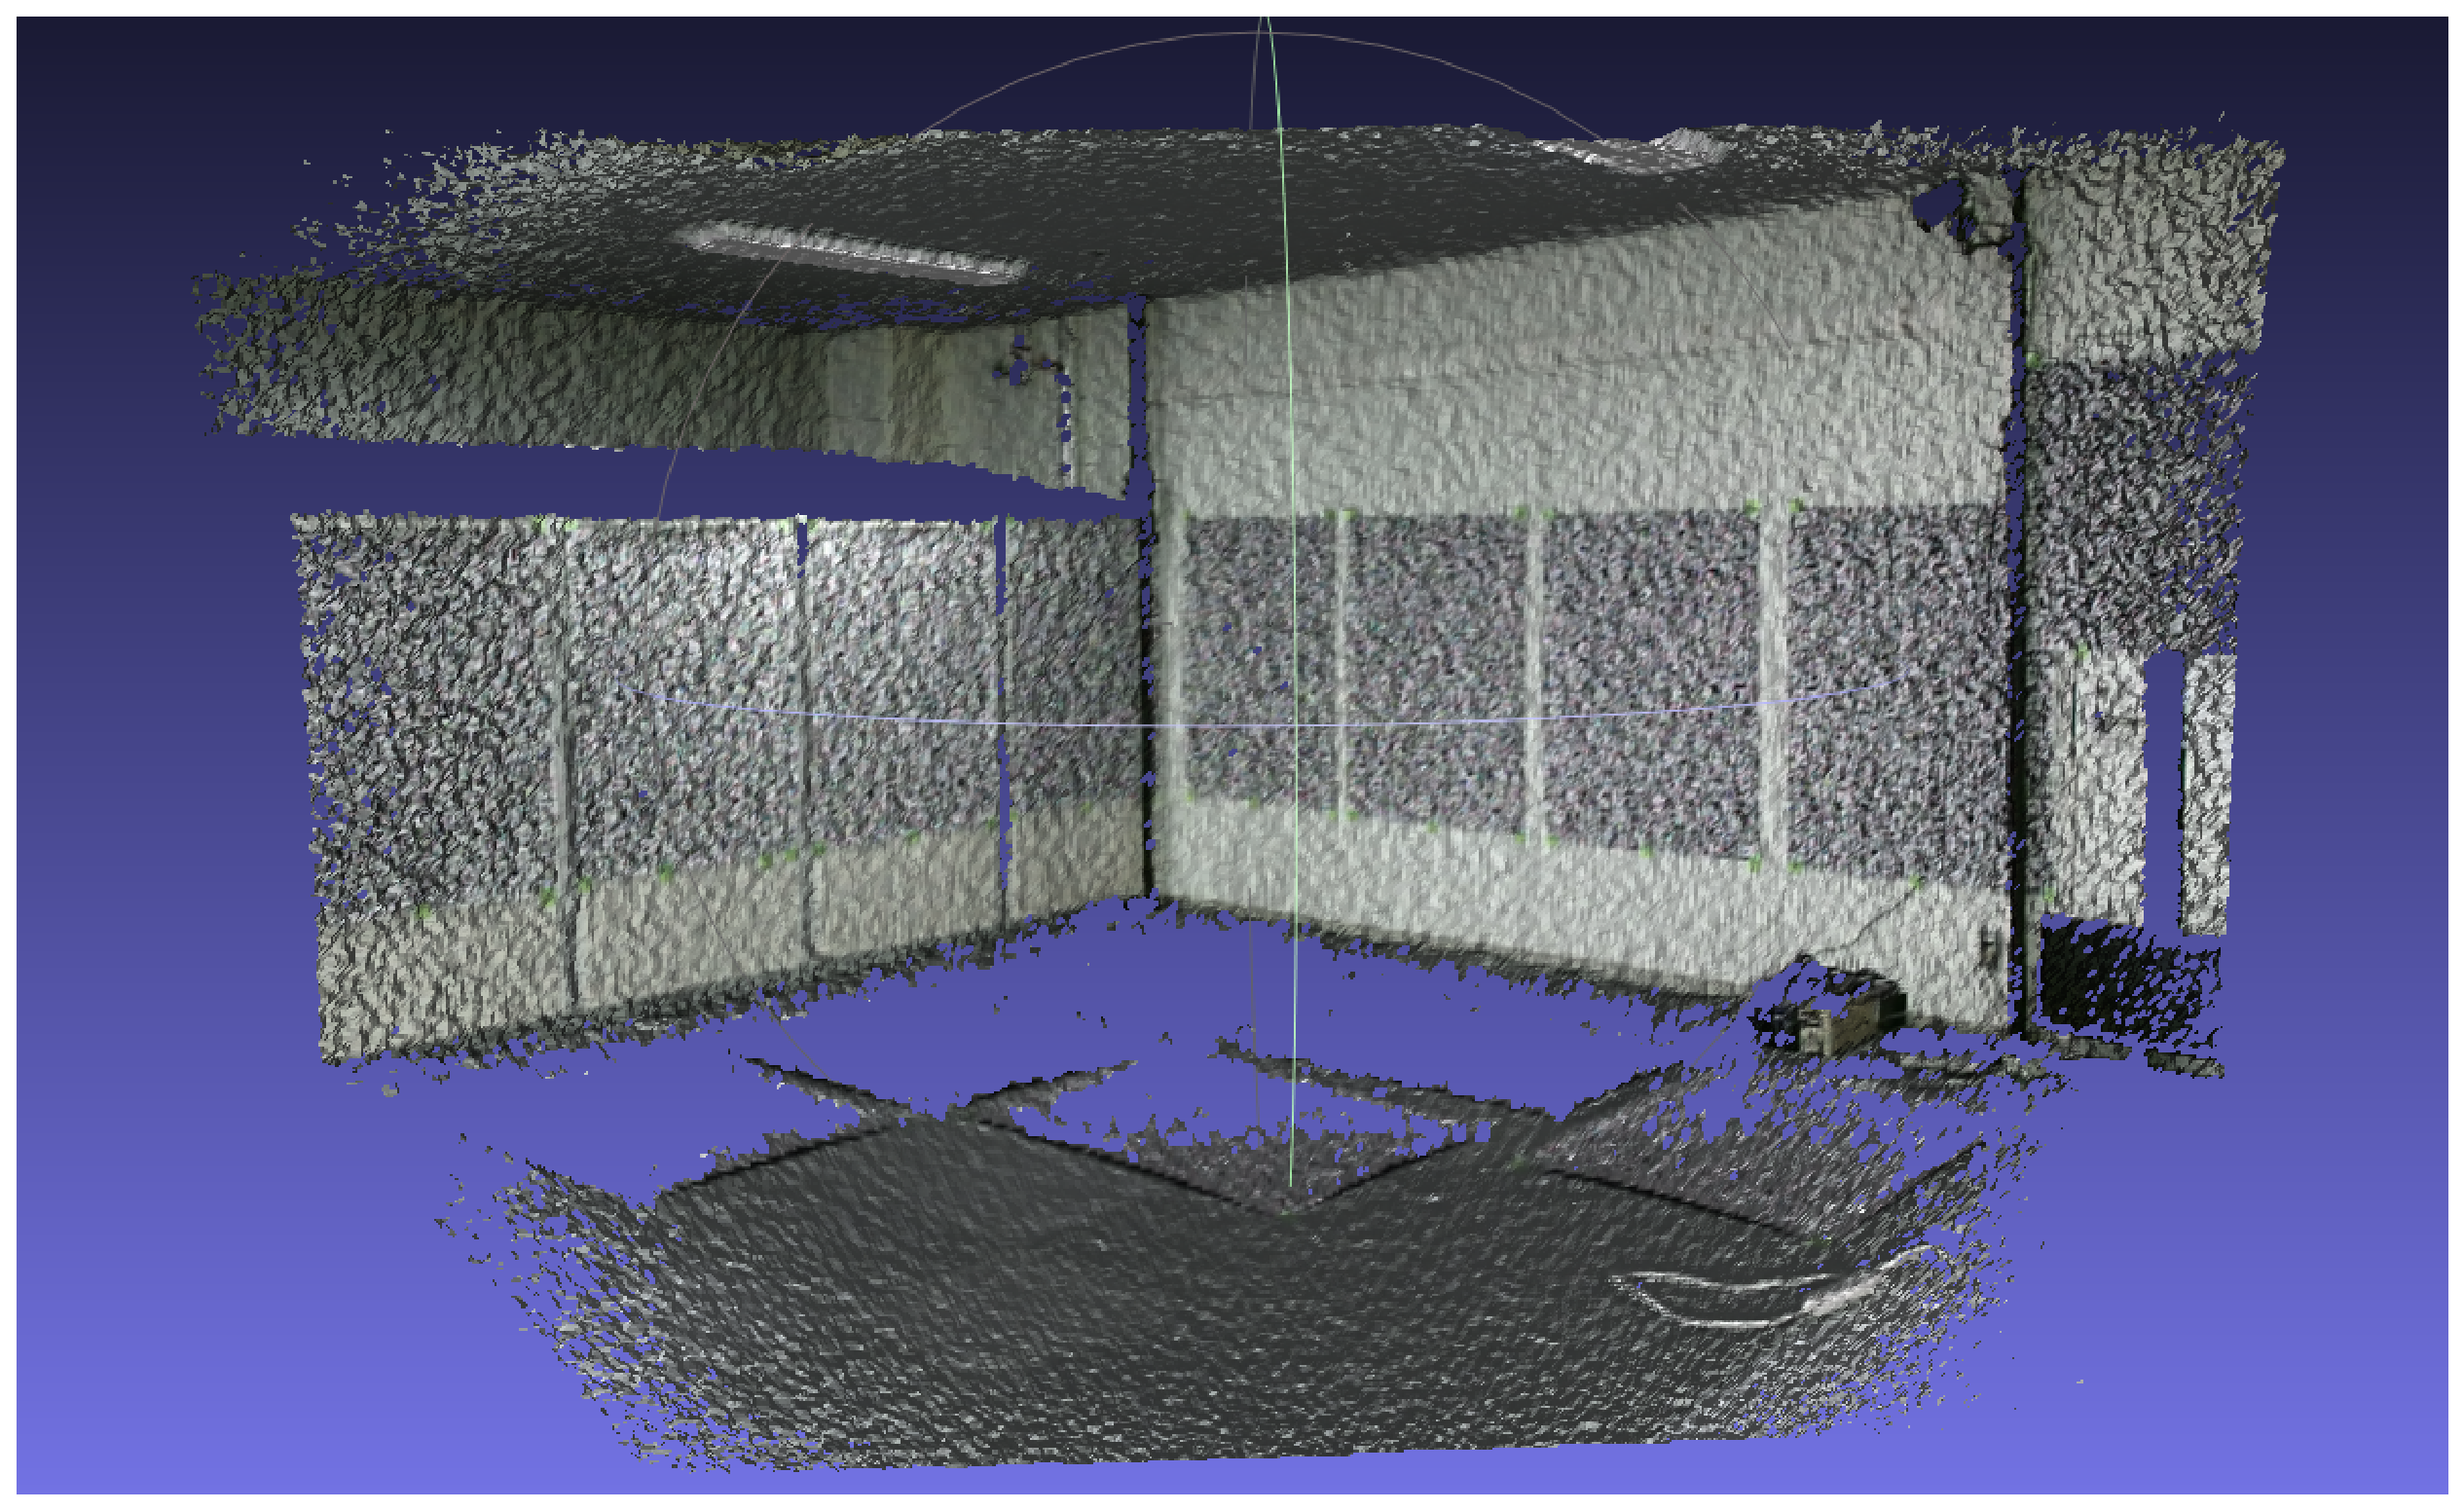
\includegraphics[height=50mm]{figure/RGB-D画像.eps}
   \caption{RGB-D画像}
   \label{RGB-D画像}
  \end{center}
\end{figure}

\newpage

\vspace{5mm}
ステレオ画像とRGB-D画像を比較すると,RGB-D画像の方が精度が良いことが分かる.今回測定したRGB-DカメラはKinect V2である.Kinect V2測定可能距離が最大8mである反面,ステレオカメラは最大20mまで測定可能である.また,Kinect V2の場合,測定可能水平角度が70°であるが,ステレオカメラは89°である.さらに後述のように,Kinect V2は太陽光の影響を受けやすい.このため,屋外ではステレオ画像を用いる方が有利と思われる.

%--------------------------------------------------------------------------------------------------
\section{ステレオカメラを搭載した実験用台車}
本節では,ステレオカメラを搭載する台車について述べる.台車の上にはステレオカメラだけではなくステレオカメラとの比較対象となるKinect V2も載せる.まず,ステレオカメラを台車の上に載せるためにはキャリブレーションで使われたプレートではなく別のプレートにつけなければならない.図3.11に台車用のプレート設計図と図3.12にステレオカメラ取り付けのイメージを表す.また,図3.13に台車全体の取り付けイメージを表す.

\begin{figure}[h]
  \begin{center}
   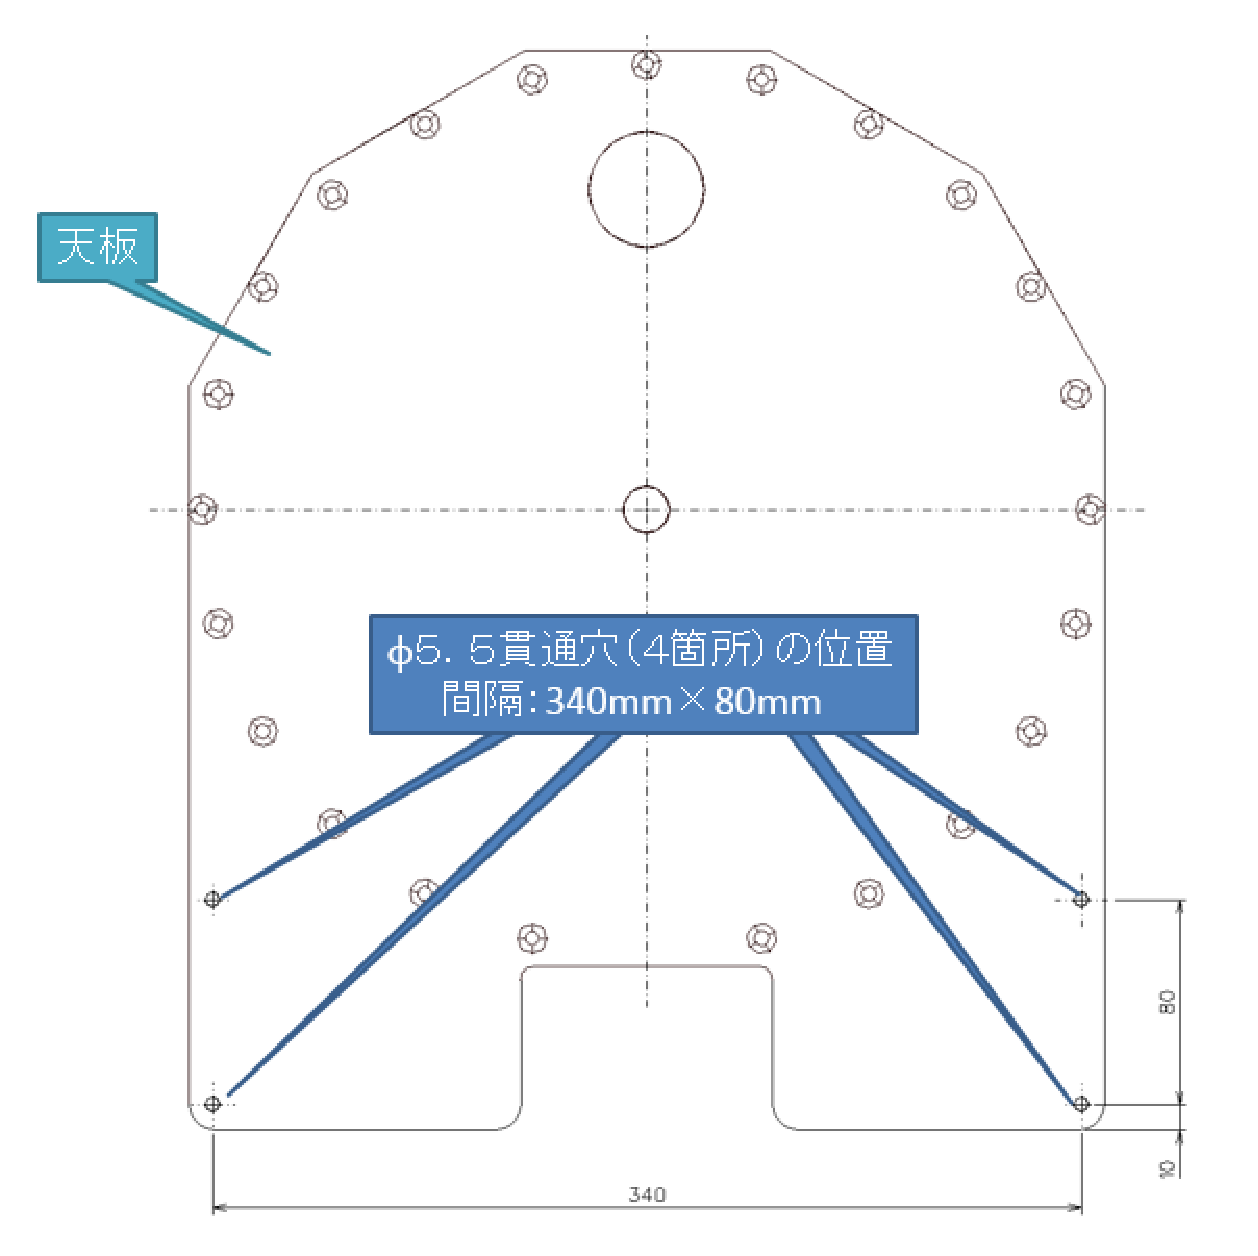
\includegraphics[height=100mm]{figure/台車用のプレート設計図.eps}
   \caption{台車用のプレート設計図}
   \label{台車用のプレート設計図}
  \end{center}
\end{figure}
\newpage
%
\begin{figure}[htbp]
  \begin{center}
   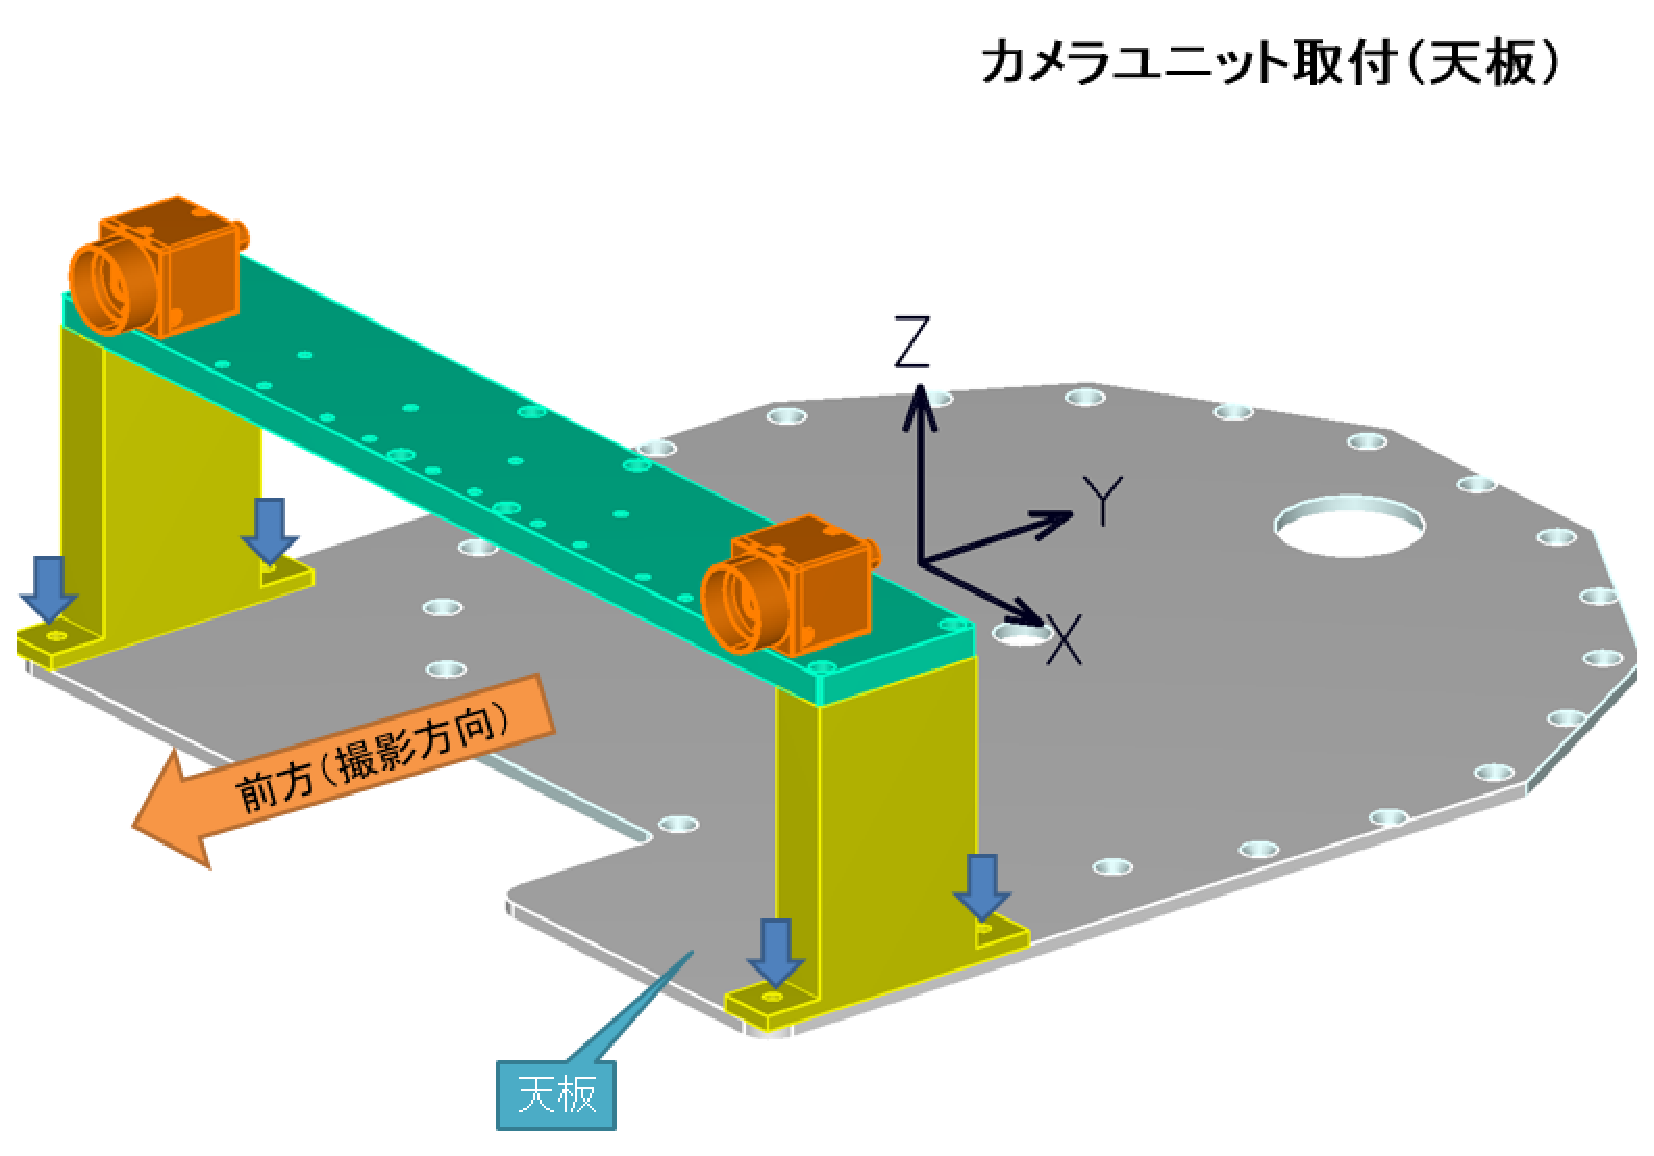
\includegraphics[height=50mm]{figure/ステレオカメラ取り付けのイメージ.eps}
   \caption{ステレオカメラ取り付けのイメージ}
   \label{ステレオカメラ取り付けのイメージ}
  \end{center}
\end{figure}

\begin{figure}[htbp]
  \begin{center}
   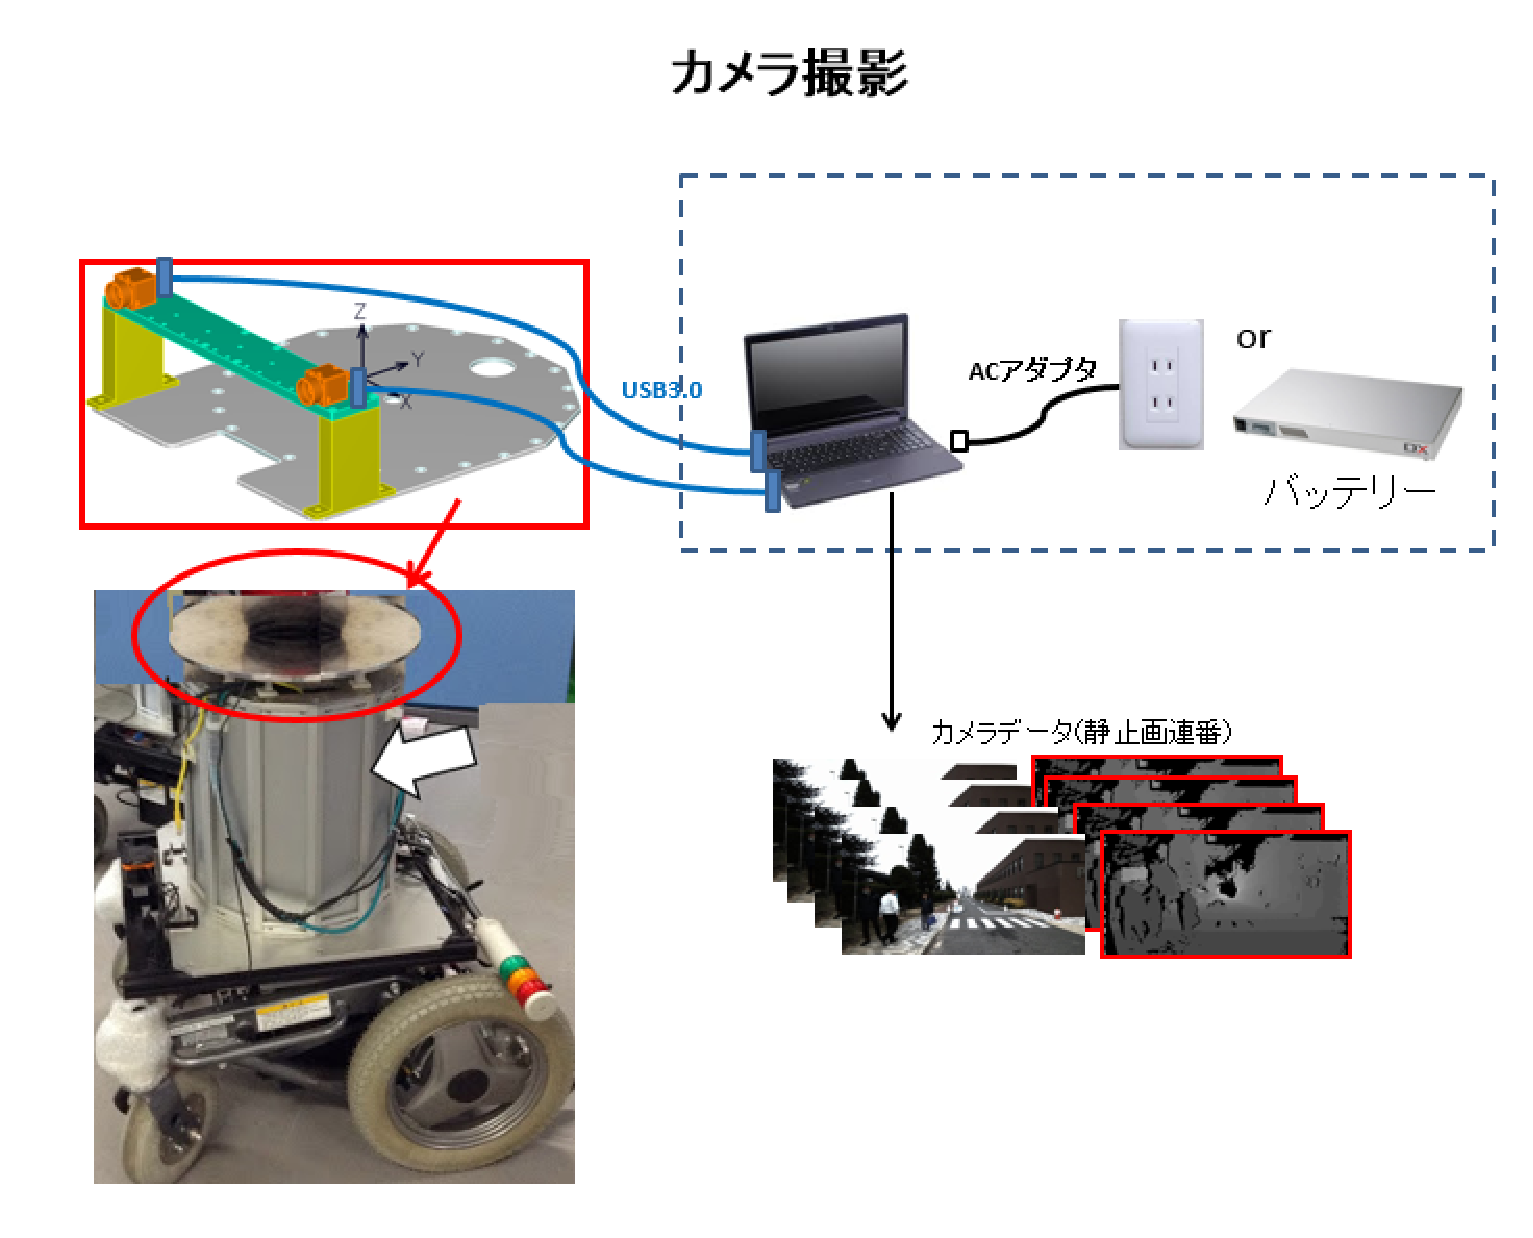
\includegraphics[height=60mm]{figure/台車全体の取り付けイメージ.eps}
   \caption{台車全体の取り付けイメージ}
   \label{台車全体の取り付けイメージ}
  \end{center}
\end{figure}

前述した通り,台車の上にはKinect V2も一緒に載せるが,パソコンと違い,Kinect V2はバッテリが充電式でないためアダプターを切って,バッテリを繋げる作業がいる.図3.14に実際バッテリを繋げたものを表す.図3.14の左からKinect V2のアダプター,DC-DCコンバーター,バッテリとなる.最後に,実際実験に用いる台車のキャッチャーを図3.15に表す.ステレオカメラの上に球を載せる理由は台車の位置計測のためである.


\begin{figure}[htbp]
  \begin{center}
   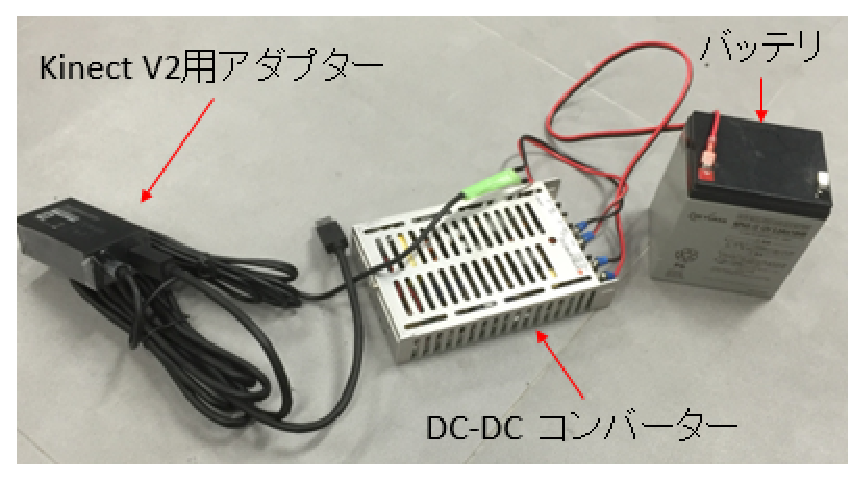
\includegraphics[height=70mm]{figure/battery_kinectV2.eps}
   \caption{バッテリ式Kinect V2}
   \label{battery_kinectV2}
  \end{center}
\end{figure}

\begin{figure}[htbp]
  \begin{center}
   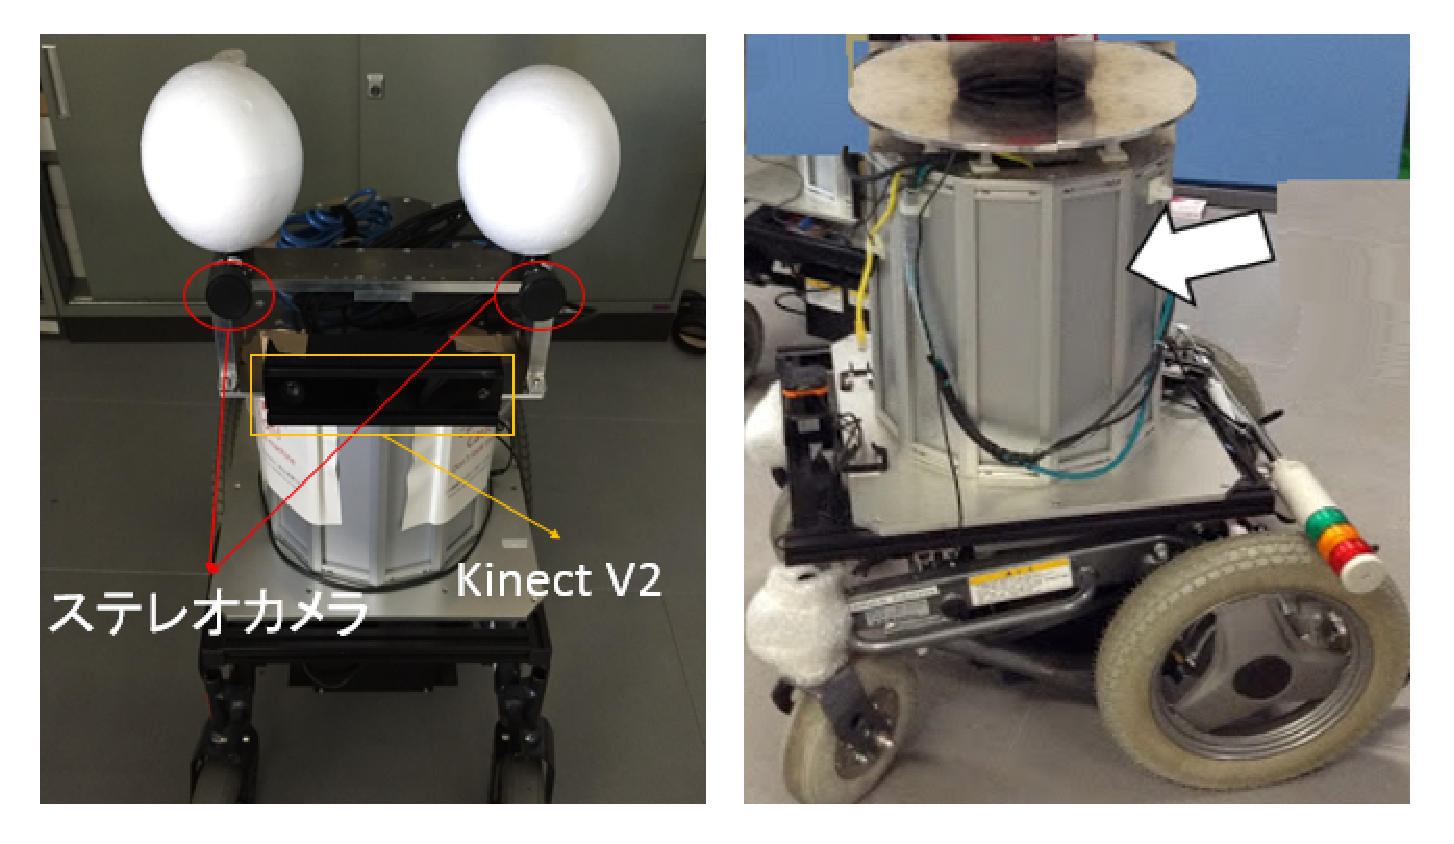
\includegraphics[height=90mm]{figure/台車.eps}
   \caption{台車}
   \label{台車}
  \end{center}
\end{figure}
\newpage

%--------------------------------------------------------------------------------------------------

\section{環境地図}
本節では,ステレオカメラで撮った計測データを用いて位置同定を行う際,必要となる環境地図データの取得法とステレオカメラで撮った場所つまり台車の真値計測法について述べる.

\subsection{環境地図の取得法}
まずは,環境地図の取得法である.環境地図は前述した通り,3次元レーザスキャナFARO Focus 3D (以降FAROと表記)を用いて撮る.FAROは高精度,高密度な点群とカラー画像が取得可能である.またパラメータとしては解像度と品質があり,状況によって調整可能である.解像度は360度を何ポイント計測するかで撮影距離と計測時間に影響がある.品質は同じポイントを何回計測するかでノイズと計測時間に影響がある.図3.16にFAROを表す.

\begin{figure}[htbp]
  \begin{center}
   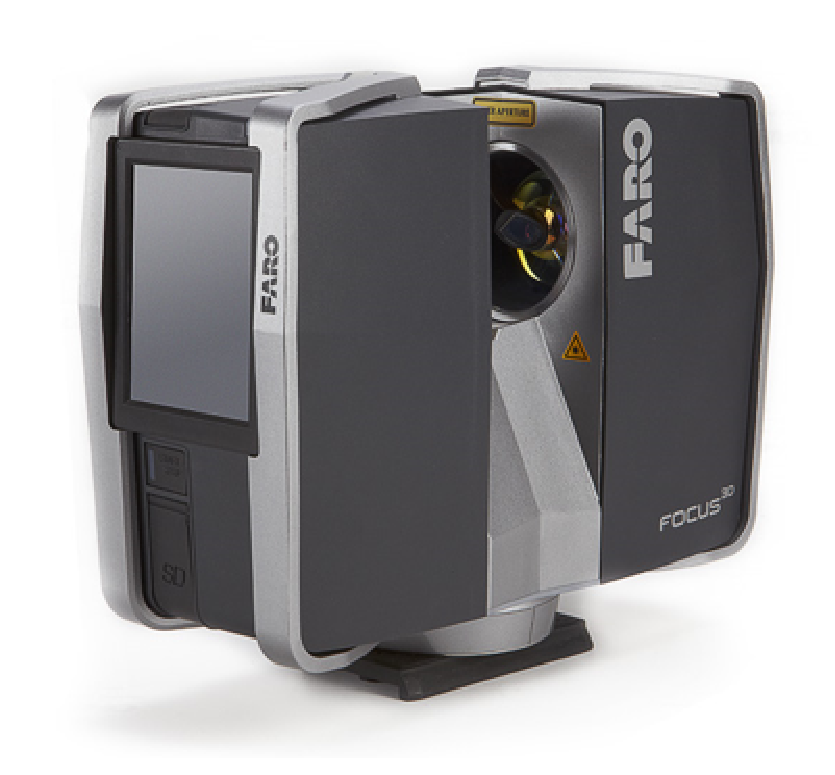
\includegraphics[height=70mm]{figure/FARO.eps}
   \caption{FARO Focus 3D}
   \label{FARO}
  \end{center}
\end{figure}

FAROのパラメータを設定してスキャンデータを撮ると,位置同定プログラムを動かすためにPTX形式に変える必要がある.スキャンデータをPTX形式に変えるときはSCENEというソフトを使う.SCENEはFAROで撮ったスキャンデータを可視化,色々な形式にエクスポート,その以外にも様々な機能がある.図3.17に解像度1/5,品質x2の地図データの例を表す.また,図3.18にはボクセル化された地図データの例を表す.

\begin{figure}[htbp]
  \begin{center}
   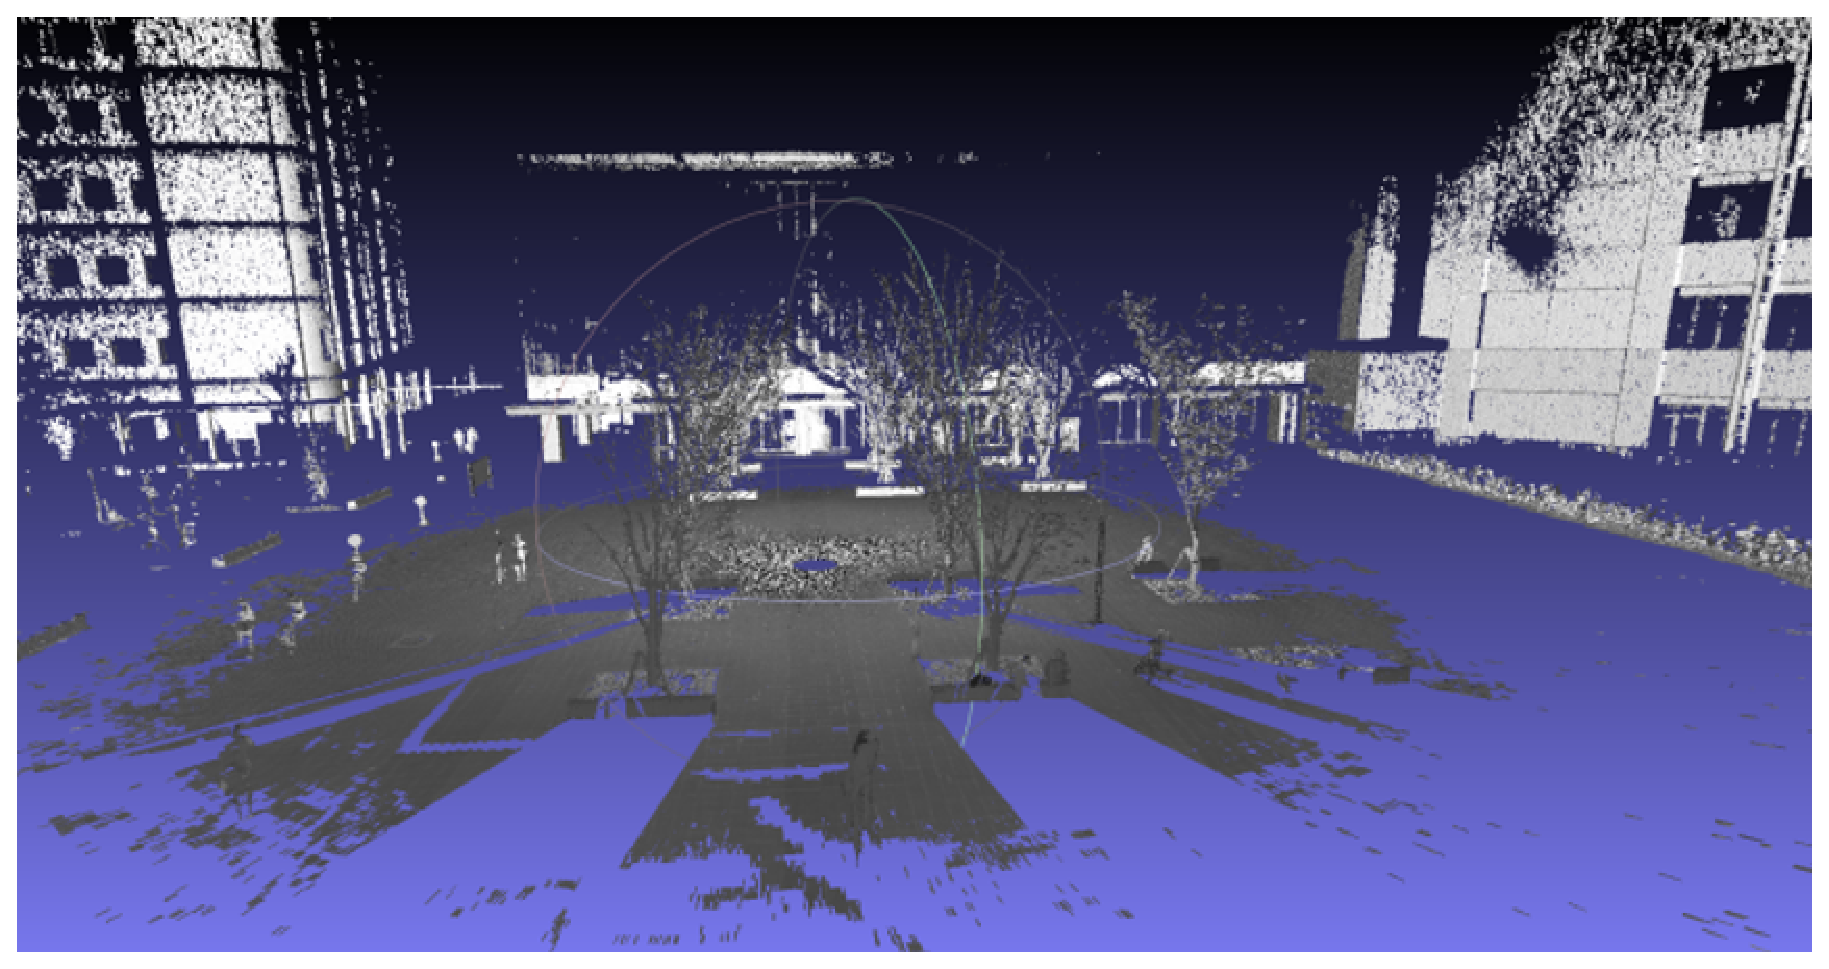
\includegraphics[height=80mm]{figure/地図データ(PTX).eps}
   \caption{地図データ(PTX)}
   \label{地図データ(PTX)}
  \end{center}
\end{figure}

\begin{figure}[htbp]
  \begin{center}
   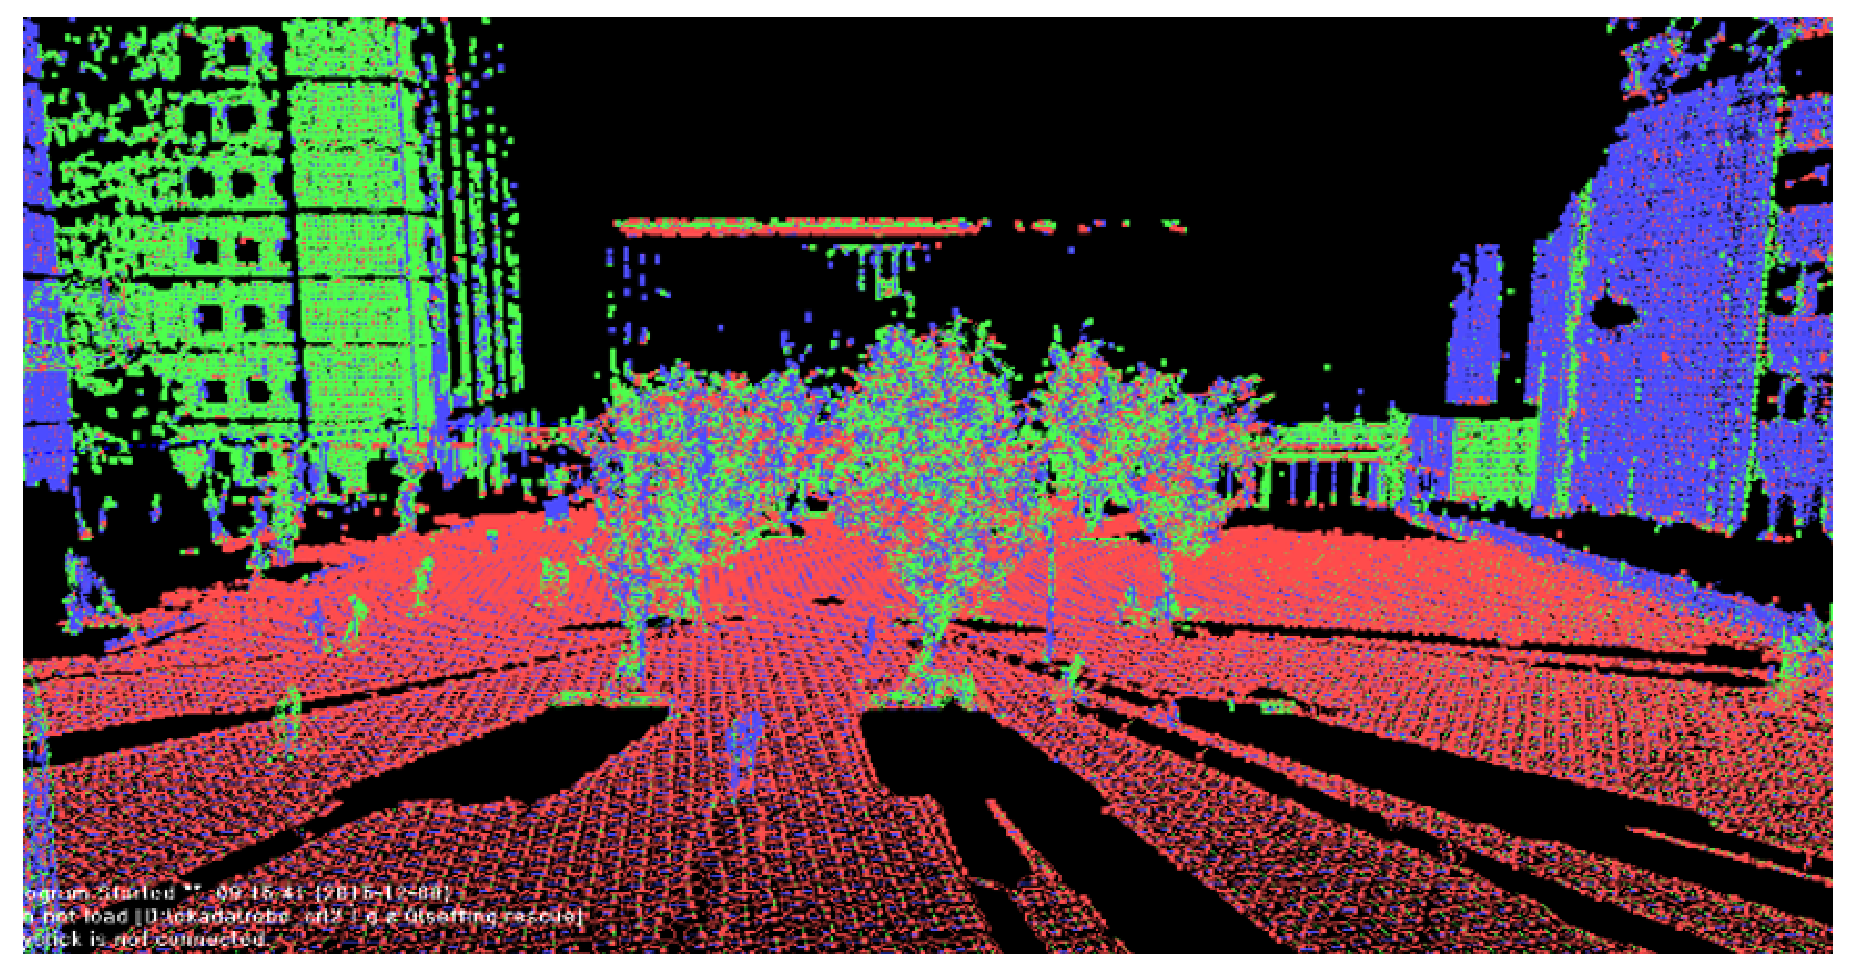
\includegraphics[height=80mm]{figure/地図データ(Voxel).eps}
   \caption{地図データ(Voxel)}
   \label{地図データ(Voxel)}
  \end{center}
\end{figure}

\vspace{15mm}
データの真ん中を見ると丸い穴があるが,これはFAROが実際置かれたところでFAROの真下が撮れていないため表れる死角である.撮れた地図データは前述の通り,SCENEソフトを用いてPTX形式化することで位置同定プログラムを動かす際の地図データができる.

\subsection{台車の位置計測法}

地図データと計測データを用いて位置同定を行い,パーティクルフィルタのリサンプリング100回目の収束位置を推定された位置とする.ただし,位置同定精度の性能を比較するためには,台車の位置計測値が必要となる.そこで,本章では台車の位置計測法について述べる.\par
まずは,地図データを撮ったFAROの位置で電源をONにしたまま,計測データを撮る台車を撮る.電源をONしたまま,続いて台車の位置を撮る理由は,FAROは電源の切り替えにより,FAROのX,Y座標軸が変わるからである.前述の通り,ステレオカメラの上に球を載せる理由は台車の位置計測ためと述べたが,SCENEソフトを用いると球の認識ができ,SCENEソフト上で球の座標値が分かる.SCENEソフトで球を認識し,座標値を出したキャッチャーを図3.19に表す.図3.19の右側のPositionというところに球の座標値が出る.

\begin{figure}[htbp]
  \begin{center}
   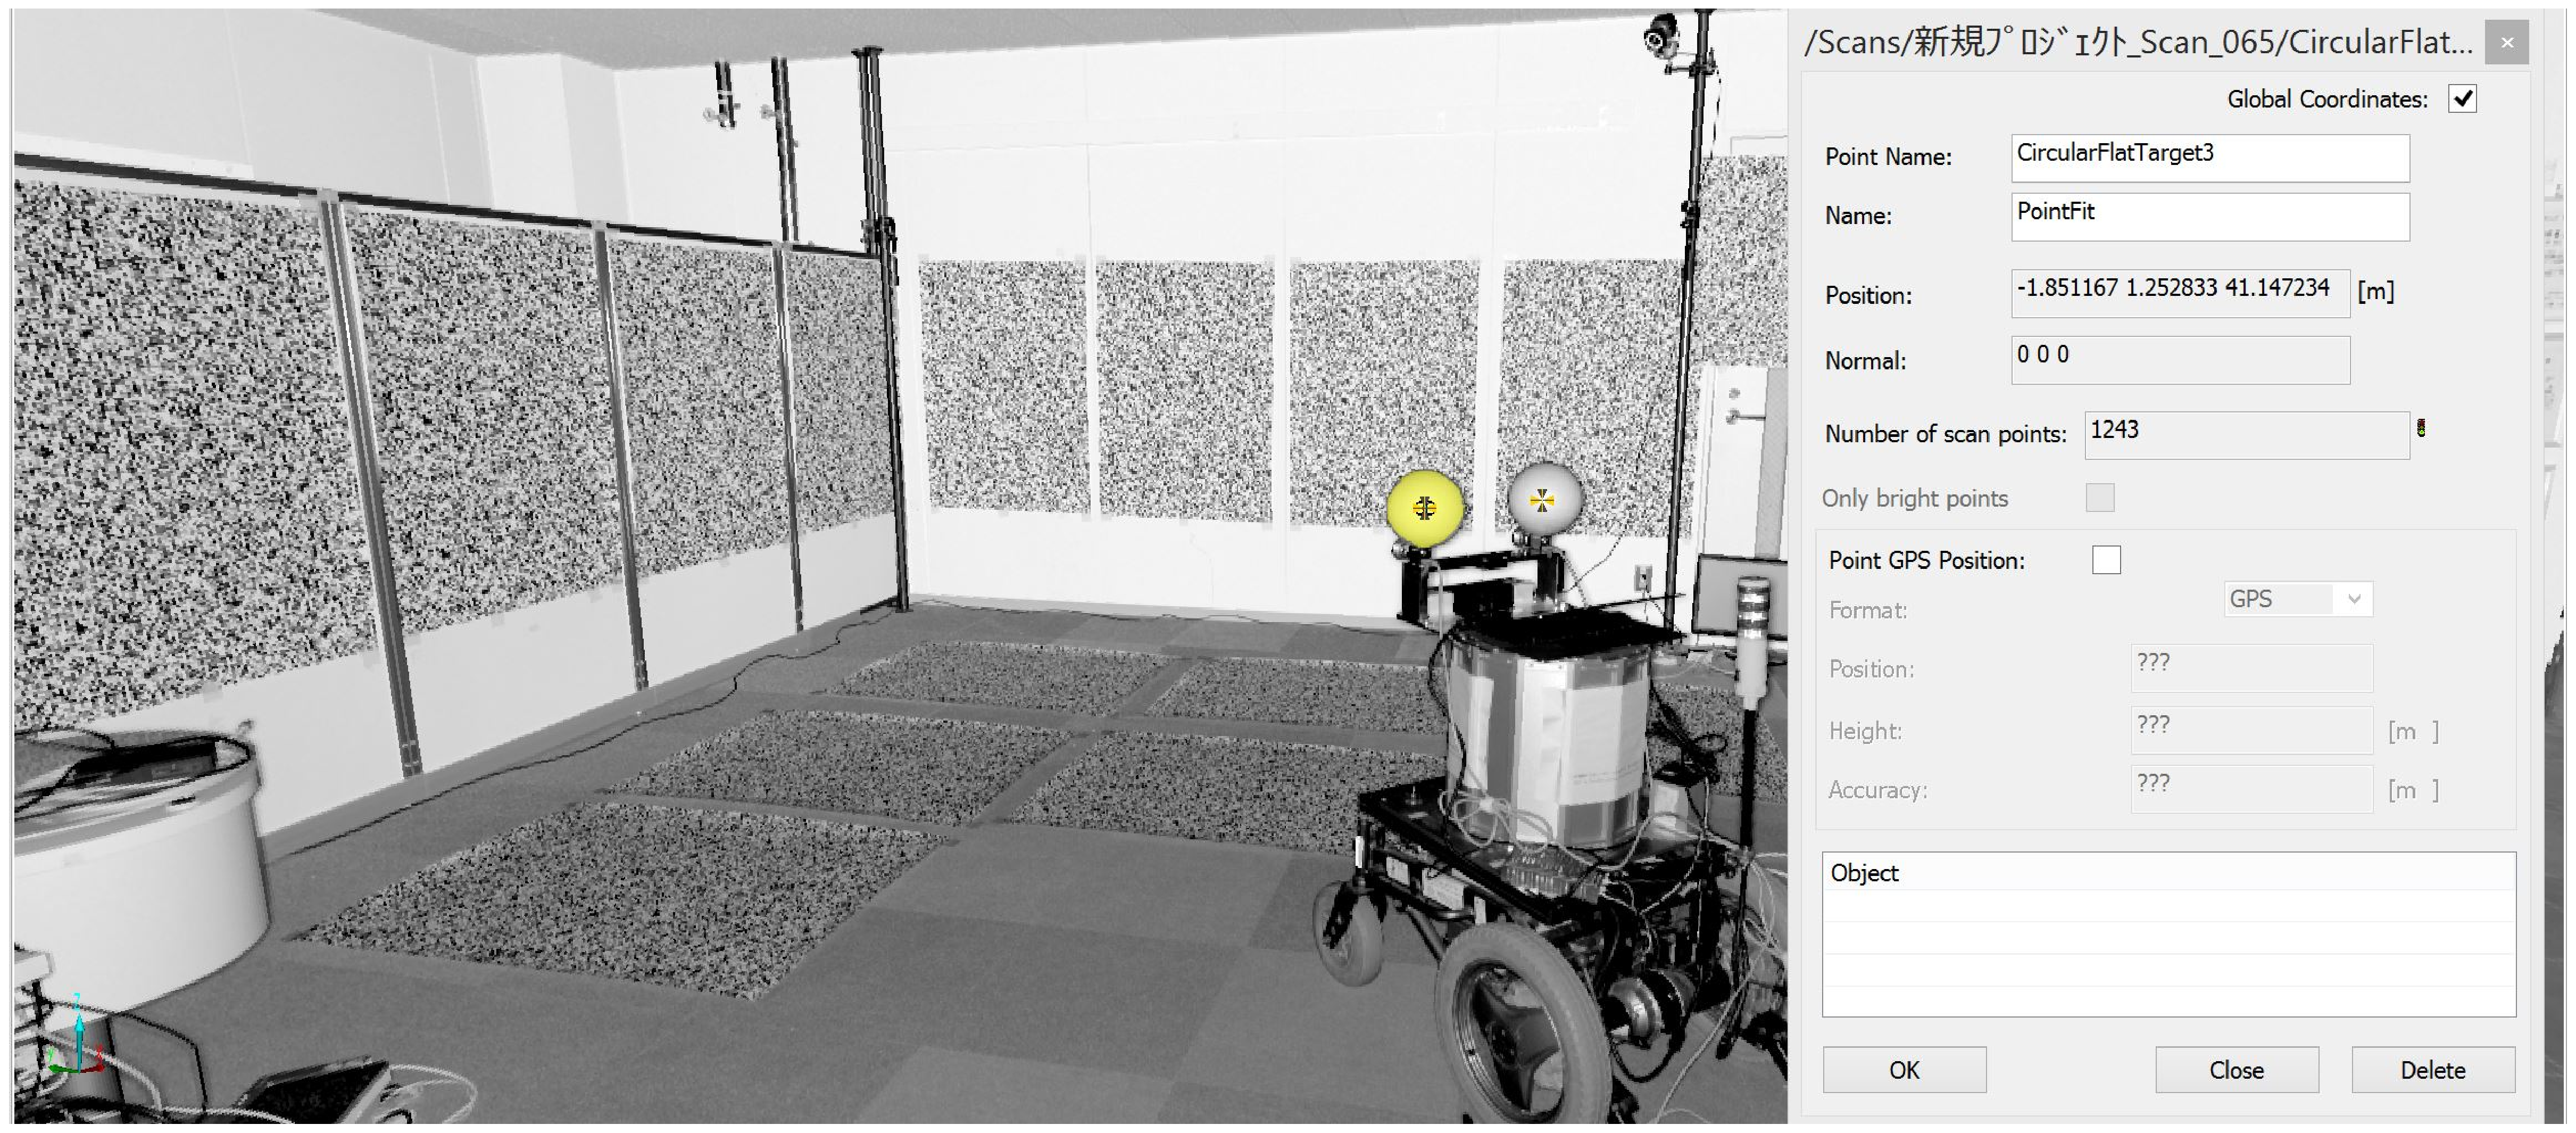
\includegraphics[height=70mm]{figure/球の認識.eps}
   \caption{球の認識}
   \label{球の認識}
  \end{center}
\end{figure}
\newpage

左右のステレオカメラの球座標から球の半径をZ軸に引いた値がステレオカメラの座標値となる.左のステレオカメラの座標値が計測データの真値となる.右ステレオカメラの球は左のステレオカメラの真値との計算を通して,方向を求めるために用いられる.つまり,計測データを撮る際はFAROからステレオカメラの上にある球が重ならないように注意するべきである.左ステレオカメラの座標値を($X_{l}$,$Y_{l}$,$Z_{l}$),右ステレオカメラの座標値を($X_{r}$,$Y_{r}$,$Z_{r}$)とすると,ステレオカメラの方向$D_{s}$は以下のように求められる.後,FAROから台車計測時の注意を図3.20に表す.

\begin{equation}
D_{s} = -1*\cfrac{X_{r}-X_{l}}{Y_{r}-Y_{l}} = \cfrac{X_{l}-X_{r}}{Y_{r}-Y_{l}}
\end{equation}

\begin{figure}[htbp]
  \begin{center}
   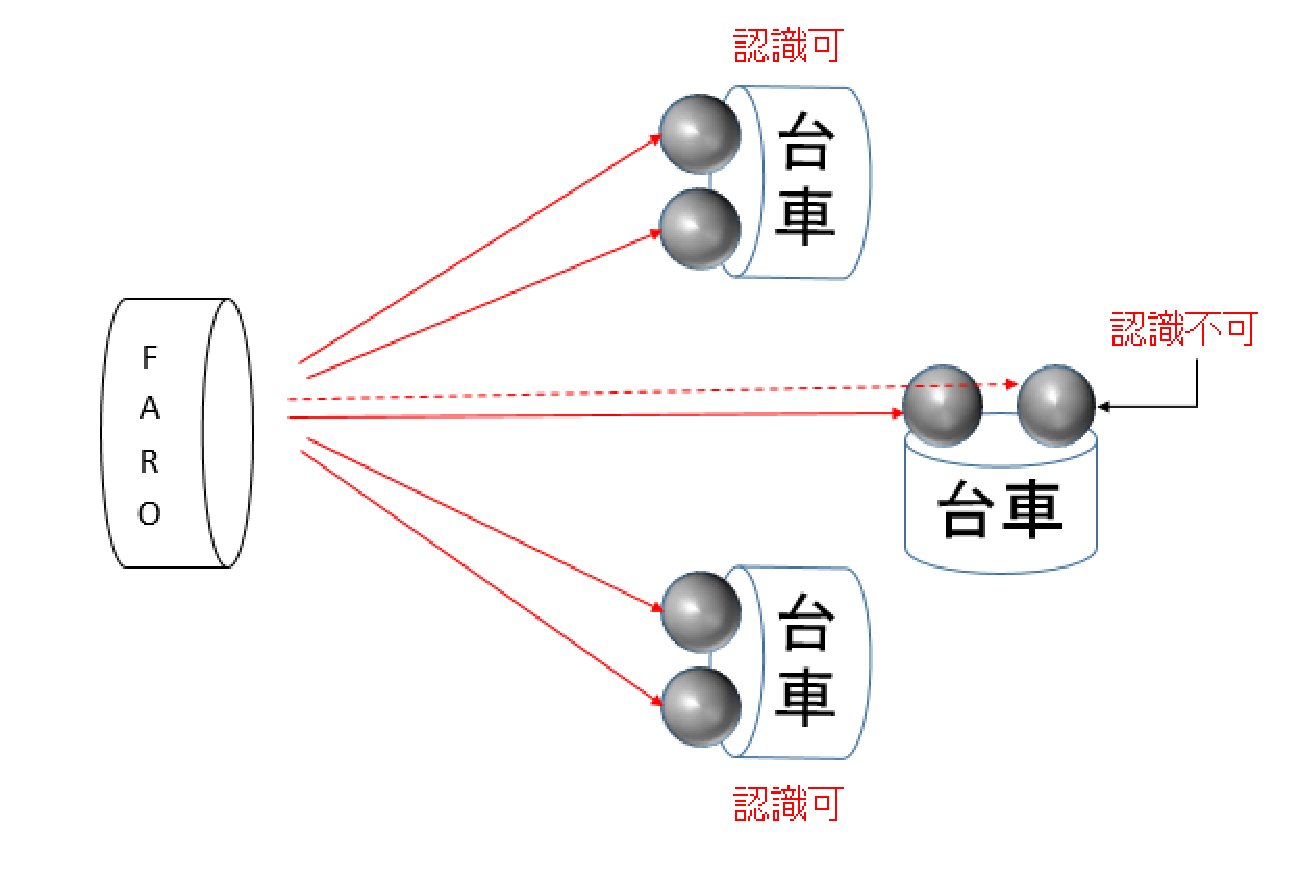
\includegraphics[height=70mm]{figure/撮影注意.eps}
   \caption{撮影注意}
   \label{撮影注意}
  \end{center}
\end{figure}

%---------------------------------------------------------------------------------------------------

%===================================================================================================
%===================================================================================================
\chapter{計測実験と評価}
%---------------------------------------------------------------------------------------------------
\section{概要}
本研究の位置同定実験には大きく屋内実験と屋外実験に分けられる.\par
まず,屋内実験では壁に人為的にテクスチャ画像を張らない通常の屋内環境でステレオカメラを用いて実験し,位置同定精度を評価する.次に,屋内は屋外に比べるとステレオカメラが認識できる特徴が少ないため,特徴を人為的な作ったテクスチャーを壁などに貼ったまま実験を行い,位置同定精度評価する.屋内実験により最も位置同定の効率かつ精度良いパラメータ設定を求める.パラメータの種類としてはボクセルの大きさと地図・計測データのオーバーラップ有無がある.最後に,屋内実験ではKinect V2との精度比較をするため,ステレオカメラの位置同定が効率・精度良く収束できるパラメータに設定した状態で,テクスチャーを貼ったまま,Kinect V2との比較実験を行い,位置同定精度評価する.\par
屋外実験では,まず,ステレオカメラとKinect V2の日光の影響によるデータ比較実験を行い,評価する.その次に,屋内で求めた効率・精度良いパラメータに設定した状態で,屋外実験を行い,位置同定精度を評価する.最後に,屋外の一本の木の特徴を用いるだけで,位置同定が可能かについて実験を行い,評価する.一本木の実験でも屋内で求めたパラメータ設定で実験を行う.

\newpage

本研究の位置同定実験は全て,パラメータ条件を以下のようにして行う.

\begin{itemize}
\item ボクセルサイズ
\begin{itemize}
\item 80,40cm(オーバーラップ有とオーバーラップ無)
\end{itemize}
 \item パーティクル数
\begin{itemize}
      \item 初回:1000個*72方向 = 72000個
	\item 2回以降:1000個
\end{itemize}
 \item リサンプリング後の予測範囲
\begin{itemize}
      \item sigma-pos = 20[mm]
      \item 位置:現在のパーティクル かつ sigma-pos*ガウス分布
	\item sigma-ori = 2[rad]
      \item 方向:現在のパーティクル かつ sigma-ori*ガウス分布 
\end{itemize}
\item リサンプリング回数 = 100回
\item 1条件当たり5回の試行
\item オーバーラップNDボクセル
\begin{itemize}
      \item オーバーラップNDボクセルを利用(オーバーラップ有と表記)
	\item オーバーラップNDボクセルを利用しない(オーバーラップ無と表記)
\end{itemize}
\item 人為的に作成したテクスチャ
\begin{itemize}
      \item テクスチャを利用(テクスチャ有と表記)
	\item テクスチャを利用しない(テクスチャ無と表記)
\end{itemize}
\end{itemize}

\newpage

\section{屋内実験}

\subsection{テクスチャー無の屋内位置同定実験・評価}
まず,テクスチャー無の屋内実験の様子を図4.1に表す.

%
\vspace{5mm}
\begin{figure}[htbp]
  \begin{center}
   \includegraphics[height=120mm]{figure/テクスチャー無の屋内実験のキャップチャ-.eps}
   \caption{テクスチャー無の屋内実験の様子}
   \label{テクスチャー無の屋内実験のキャップチャ-}
  \end{center}
\end{figure}

\newpage

テクスチャー無の屋内位置同定実験場所をPTX形式にし,MeshLabで見たデータを図{\ref{屋内実験場所}}に表す.\par
%
\begin{figure}[htbp]
  \begin{center}
   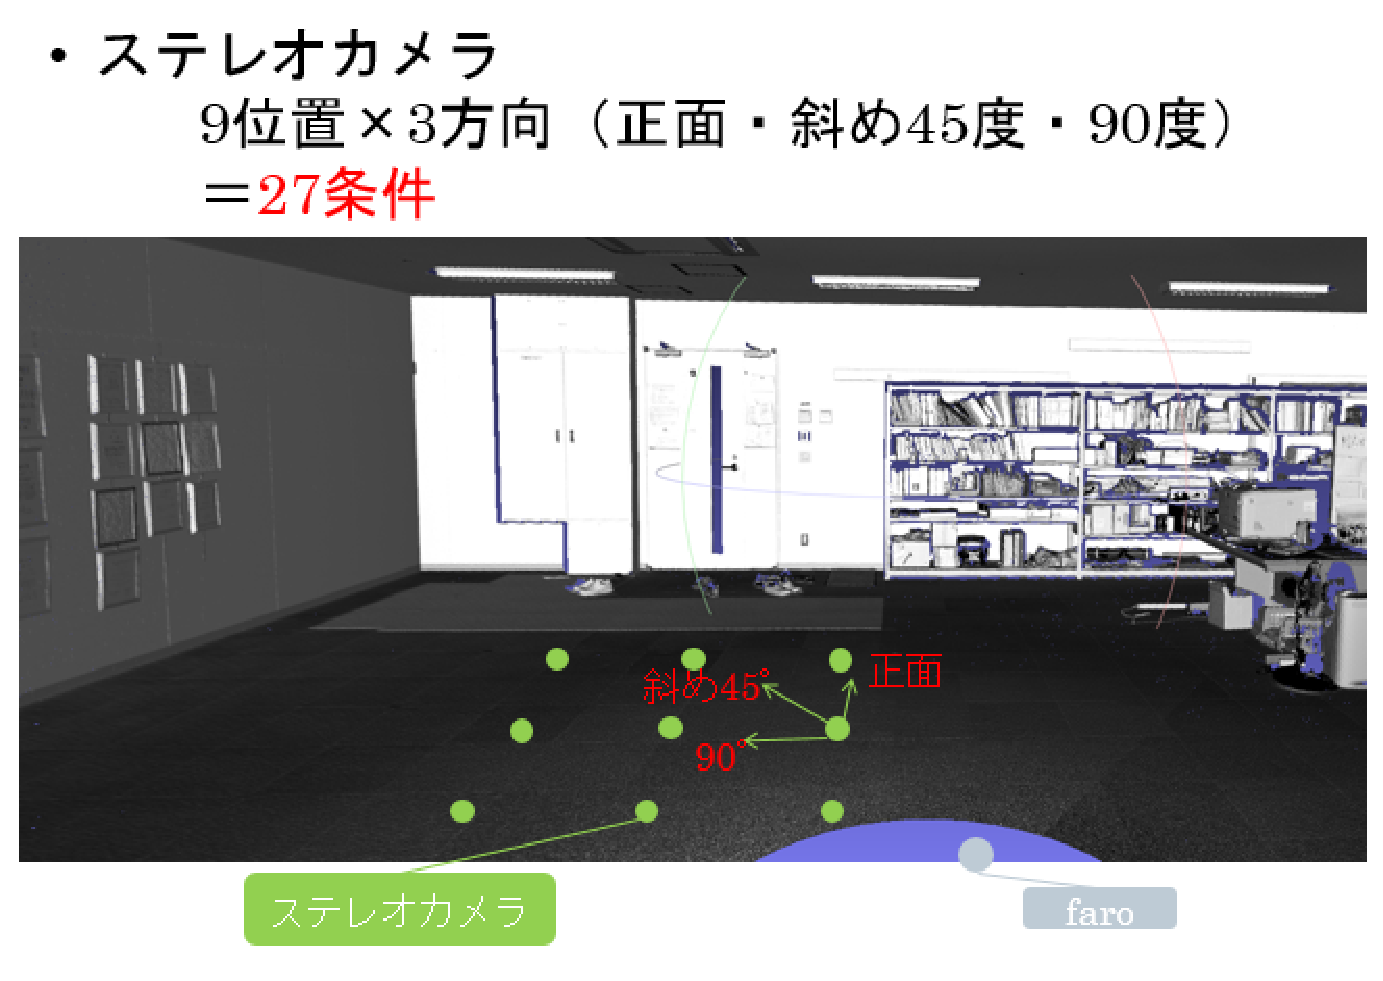
\includegraphics[height=100mm]{figure/屋内実験場所.eps}
   \caption{テクスチャー無の屋内実験場所}
   \label{屋内実験場所}
  \end{center}
\end{figure}
%

図{\ref{屋内実験場所}}のようにFAROを置いた場所は灰色の点で,ステレオカメラを用いて計測した場所は緑点の9位置である.ステレオカメラの計測は9位置から3方向(正面・斜め45度・90度),全27条件で行う.正面向きの壁からの距離は3,4,5mである.各距離で計測した計測データの例をRGB画像,PTXデータとして図{\ref{屋内計測データ例}}に表す.

\newpage
%
\begin{figure}[htbp]
  \begin{center}
   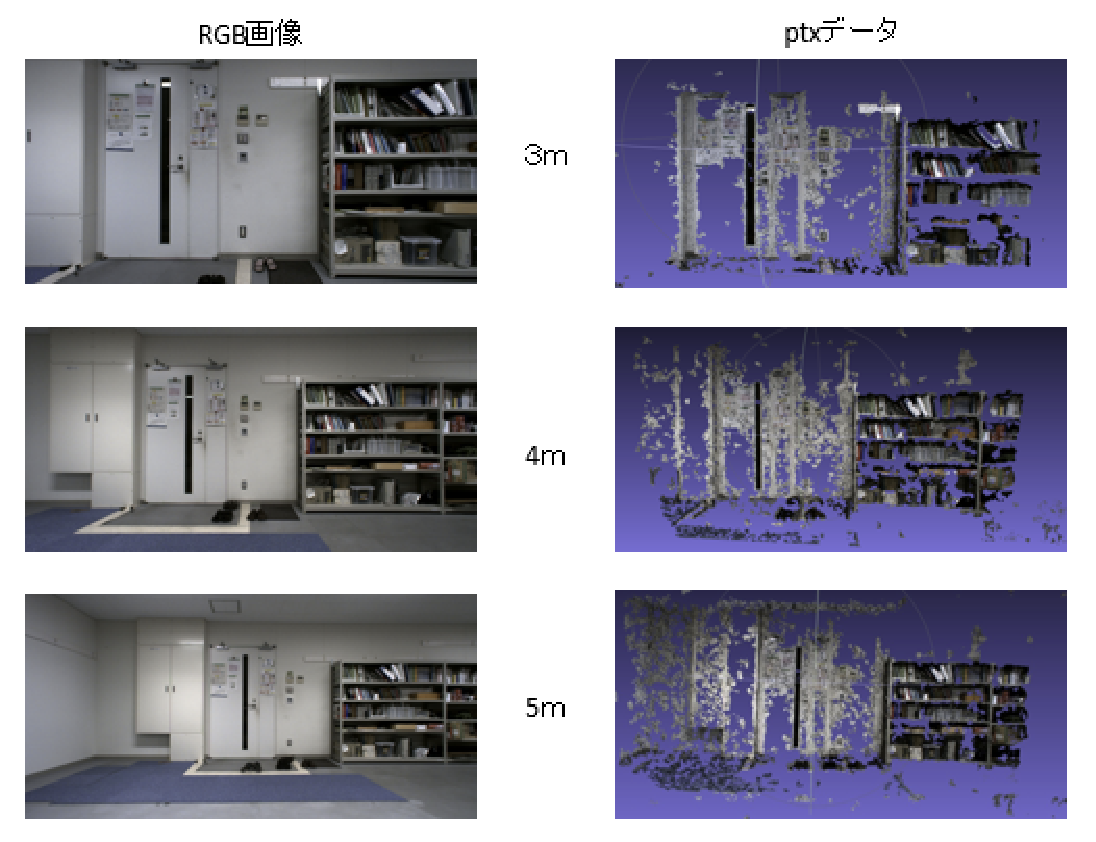
\includegraphics[height=120mm]{figure/屋内計測データ例.eps}
   \caption{テクスチャー無の屋内計測データ例}
   \label{屋内計測データ例}
  \end{center}
\end{figure}
%

位置同定プログラム上でパーティクルフィルタを使うときは乱数を与えているため,毎回同じ位置に収束するとは限らない.屋内実験の場合,地図データと計測データの収束性能を確かめるために,同じデータを用いて5回ずつ繰り返して位置同定を行い,台車の真位置から50cm以内で方向が10°以内の誤差であれば位置同定成功とみなす.本実験のパラメータの調整対象はボクセルサイズ80,40cmと地図・計測データのオーバーラップ有無となる.テクスチャー無の屋内位置同定結果をパラメータ毎に図4.4~図4.7で表す.図中の\%は試行5回中の成功率であり,右下の数字は平均の成功率(収束性能)である.



%
\begin{figure}[htbp]
  \begin{center}
   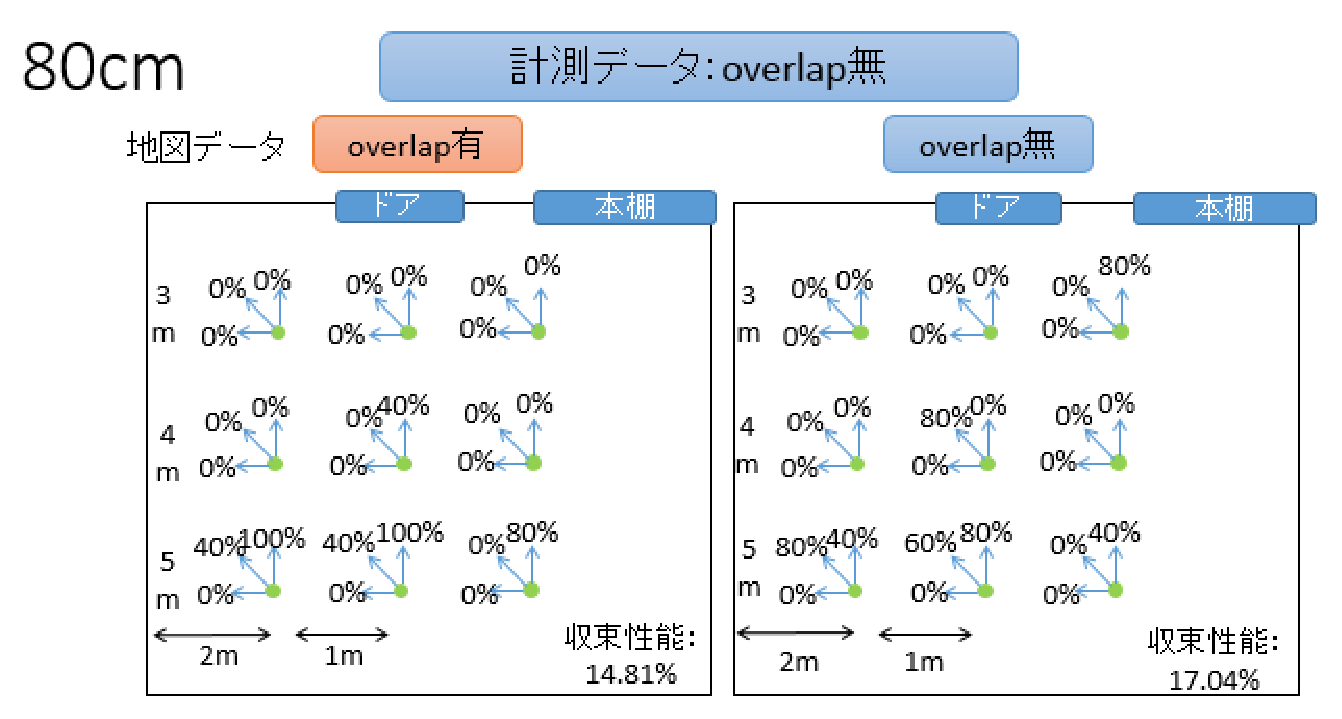
\includegraphics[height=80mm]{figure/無有無.eps}
   \caption{ボクセルサイズ:80cm,計測データオーバーラップ無かつ地図データオーバーラップ有無}
   \label{80-0}
  \end{center}
\end{figure}
%

%
\begin{figure}[htbp]
  \begin{center}
   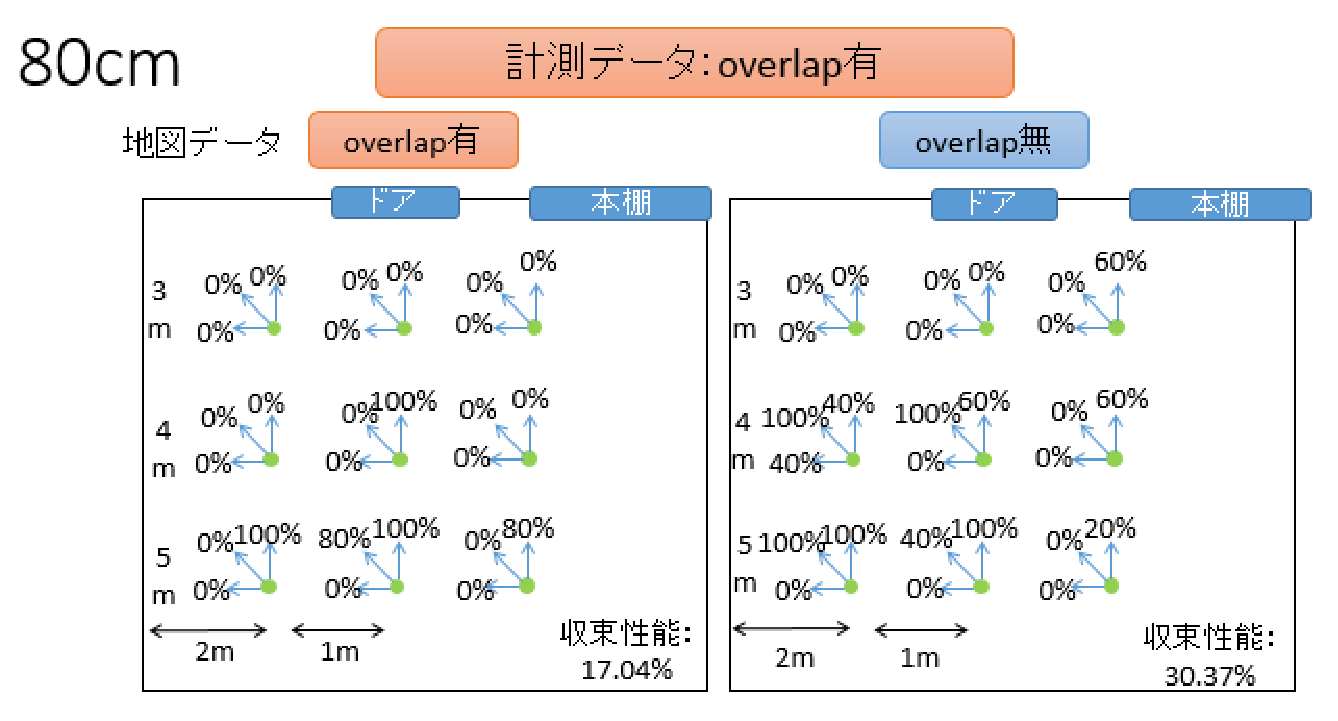
\includegraphics[height=80mm]{figure/有有無.eps}
   \caption{ボクセルサイズ:80cm,計測データオーバーラップ有かつ地図データオーバーラップ有無}
   \label{80-1}
  \end{center}
\end{figure}
%



%
\begin{figure}[htbp]
  \begin{center}
   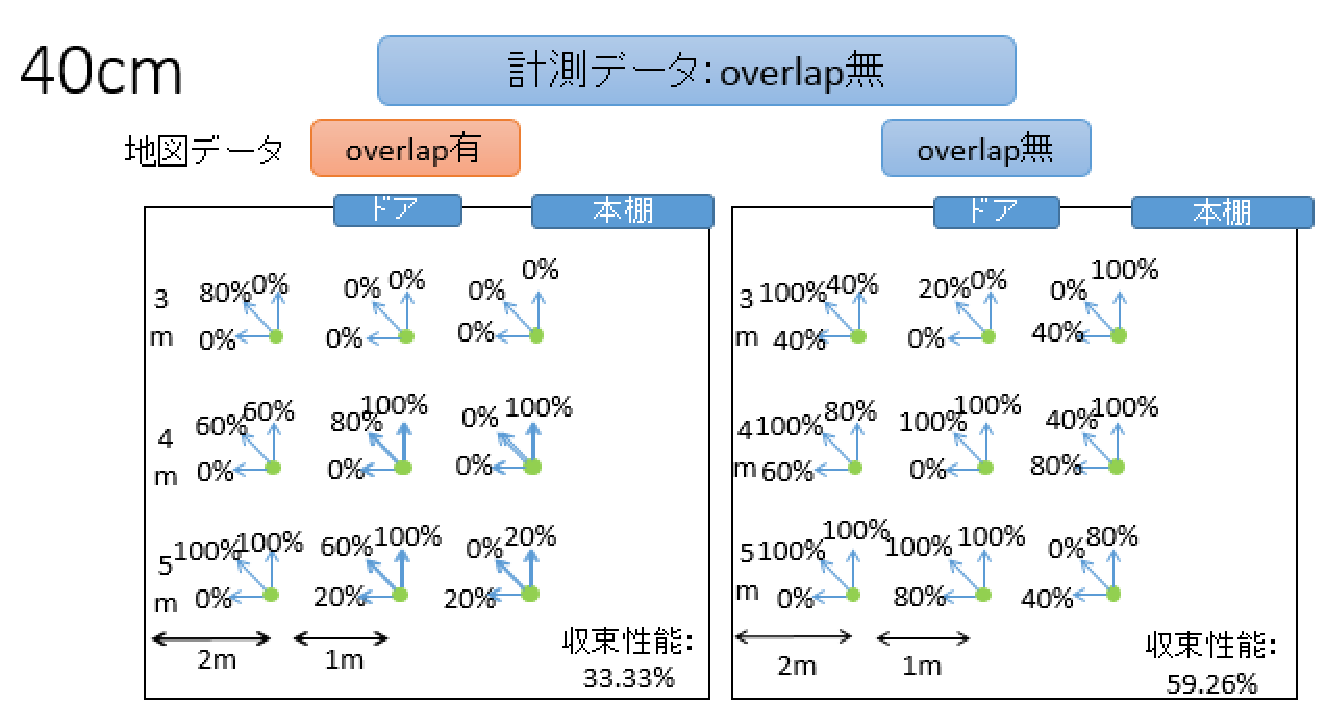
\includegraphics[height=80mm]{figure/無有無2.eps}
   \caption{ボクセルサイズ:40cm,計測データオーバーラップ無かつ地図データオーバーラップ有無}
   \label{40-0}
  \end{center}
\end{figure}
%

%
\begin{figure}[htbp]
  \begin{center}
   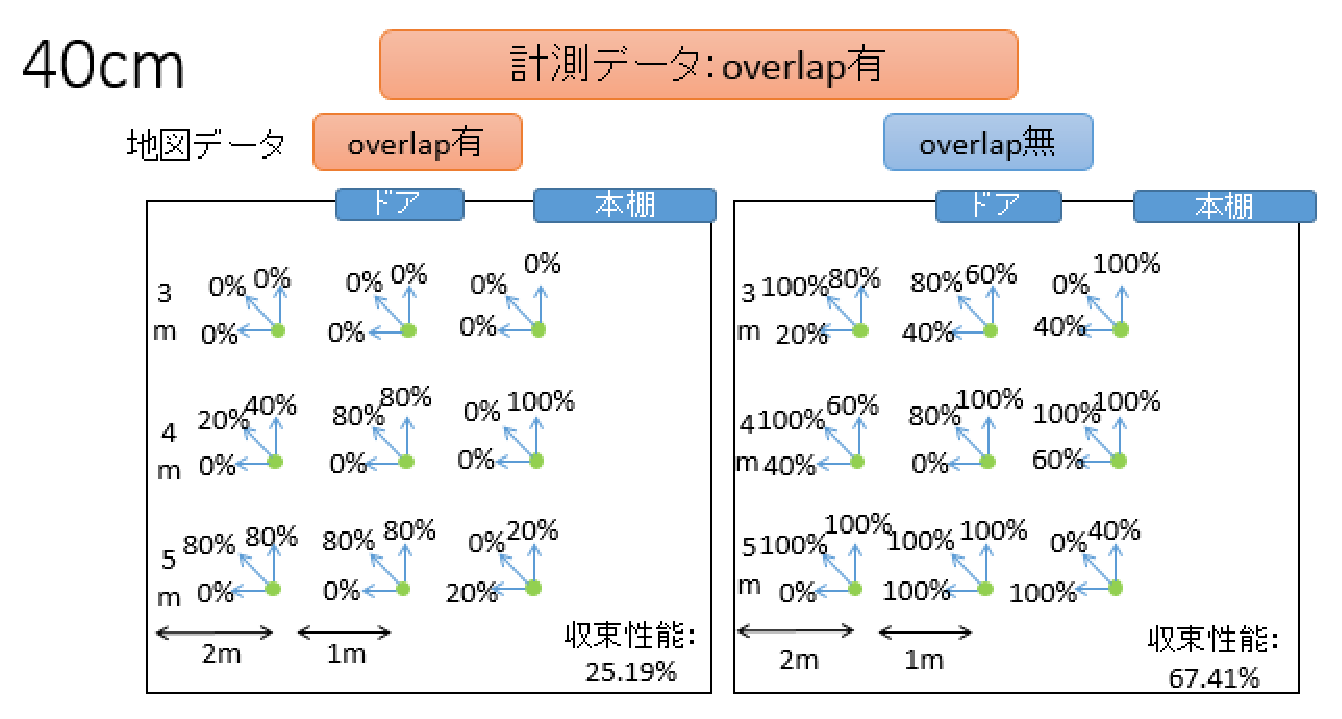
\includegraphics[height=80mm]{figure/有有無2.eps}
   \caption{ボクセルサイズ:40cm,計測データオーバーラップ有かつ地図データオーバーラップ有無}
   \label{40-1}
  \end{center}
\end{figure}
%

\newpage
図4.4~図4.7から見ると,オーバーラップの大きさが80cmの時より40cmの時がより精度が良いことが分かる.これは前述の通り,ボクセルの大きさが小さくなるほど,データの解像度が上がるからである.しかし,ボクセルの大きさが小さくなるほどボクセル数は多くなるため,計算時間が長くなる.また,正面向きの壁から距離が離れるほど精度が良くなるが,その理由は図{\ref{屋内計測データ例}}を見ると距離が離れるほど計測データの量が多くなること,および5mのデータ場合は,角が写っているため,その分距離データが含まれているからである.\par
次に,計算時間について評価する.ただしここでは計算時間の評価は,パーティクル更新時間を用いる.以下に各条件の収束性能とパーティクル更新時間を数値にまとめて表す.収束性能はプログラムを動かしたすべての回数(135回)の中で何回収束されたかを表している.パーティクル更新時間は各条件で最も精度が良かった計測データを使い,その計測データの100回リサンプリングするパーティクル更新時間の平均を取ったものである.

%
\begin{figure}[htbp]
\begin{center}
\begin{tabular}{ccc} \hline
条件 & 収束性能(\%) &  パーティクル更新時間(ms)\\ \hline \hline
80-0-0 & 17.04 & 0.049\\ \hline
80-0-1 & 30.37 & 0.324\\ \hline
80-1-0 & 14.81 & 0.359\\ \hline
80-1-1 & 17.04 & 1.621\\ \hline
40-0-0 & \bf 59.26 & 0.202\\ \hline
40-0-1 & \bf 67.41 & 1.360\\ \hline
40-1-0 & 33.33 & 0.764\\ \hline
40-1-1 & 25.19 & 5.141\\ \hline
\end{tabular}
\end{center}
\end{figure}
%
条件欄の読み方は最初にボクセルの大きさ-地図データのオーバーラップ有無(有:1,無:0)-計測データのオーバーラップ有無(有:1,無:0)である.例えば,80-0-0の場合はボクセルサイズ80cmに地図データオーバーラップ無・計測データオーバーラップ無と同じ意味になる.
上の数値からみると,収束性能が50\%以上で,計算速度が最も早い条件はボクセルサイズ40cmに地図データオーバーラップ無・計測データオーバーラップ無の時である.しかし,精度を一番重視する場合はボクセルサイズ40cmに地図データオーバーラップ無・計測データオーバーラップ有の時である.状況によってパラメータの調整は必要となることが分かる.位置同定行う際のパラメータ条件を以下のようにまとめる.条件毎に収束性能とパーティクル更新時間を比較したグラフが図4.8と図4.9となる.

%
\begin{figure}[htbp]
  \begin{center}
   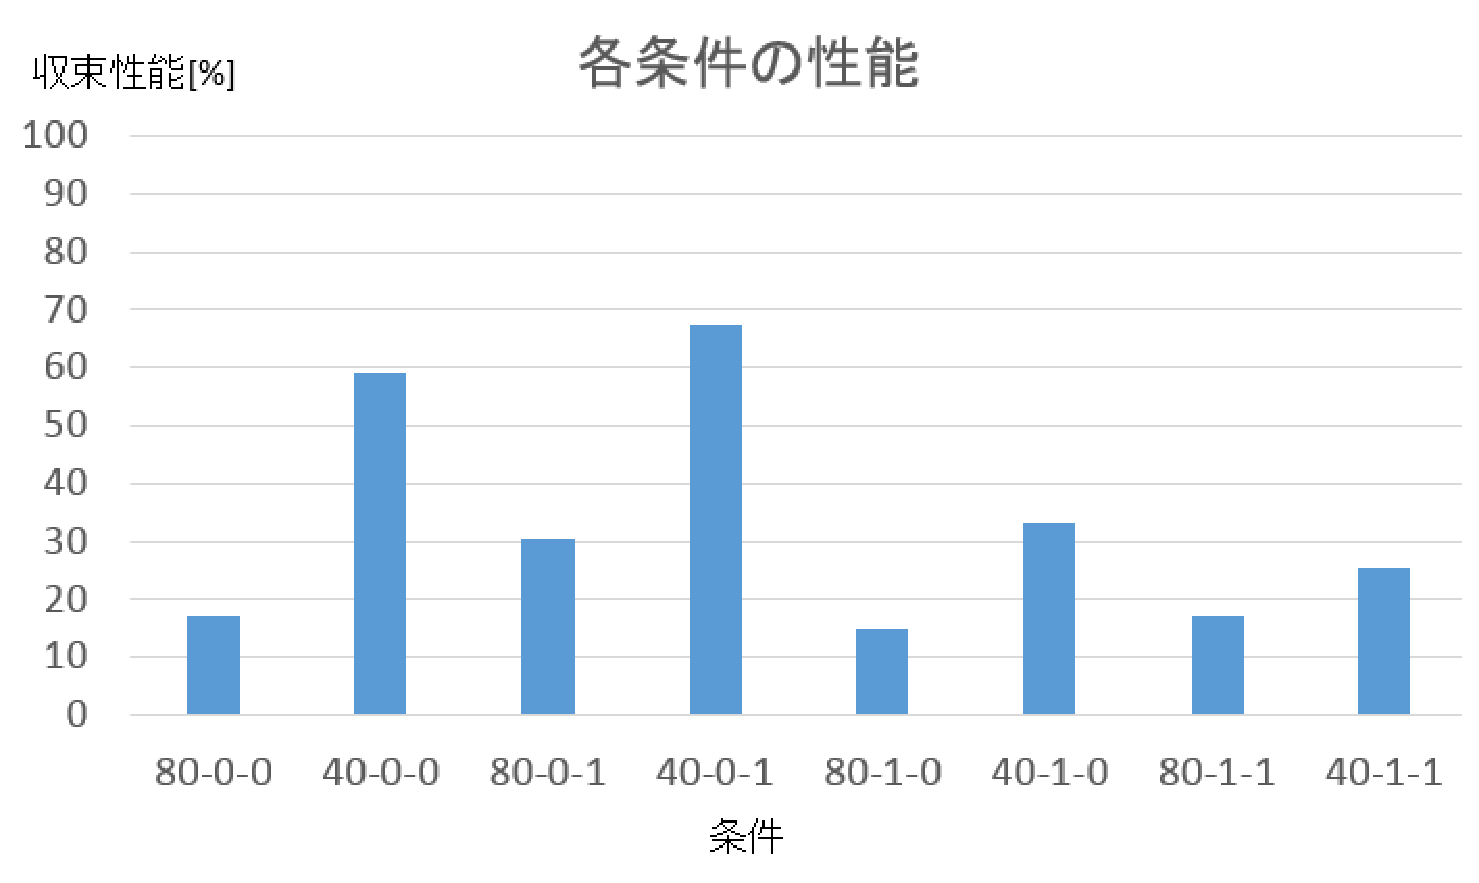
\includegraphics[height=80mm]{figure/各条件の性能.eps}
   \caption{テクスチャー無の各条件の性能}
   \label{各条件の性能}
  \end{center}
\end{figure}
%

%
\begin{figure}[htbp]
  \begin{center}
   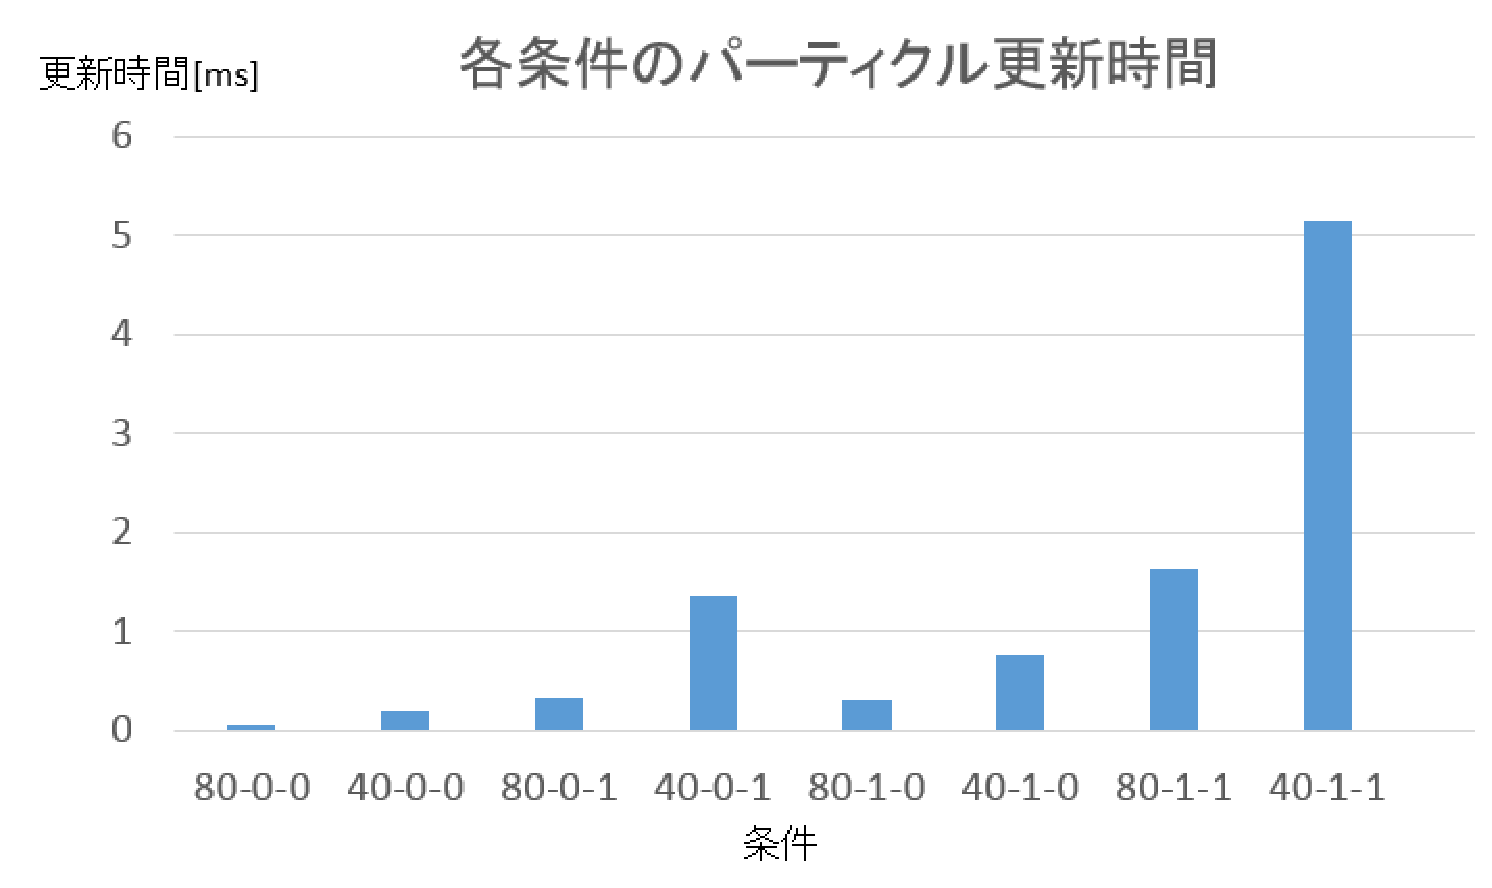
\includegraphics[height=80mm]{figure/各条件のパーティクル更新時間.eps}
   \caption{テクスチャー無の各条件のパーティクル更新時間}
   \label{各条件のパーティクル更新時間}
  \end{center}
\end{figure}
%

\newpage

ボクセルサイズ毎にオーバーラップの有無による収束性能・パーティクル更新時間の比較を見やすくするために以下のようにまとめる.ボクセルサイズ毎の地図データオーバーラップ無・計測データオーバーラップ無の時の収束性能・パーティクル更新時間を各々1とおいて,それに対する条件毎の比例数値を表している.

%
\begin{figure}[htbp]
\begin{center}
\begin{tabular}{ccc} \hline
条件 & 収束性能 &  パーティクル更新時間\\ \hline \hline
80-0-0 & 1 & 1\\ \hline
80-0-1 & 1.783 & 6.623\\ \hline
80-1-0 & 0.870 & 6.243\\ \hline
80-1-1 & 1 & 33.10\\ \hline \hline
40-0-0 & 1 & 1\\ \hline
40-0-1 & 1.138 & 6.734\\ \hline
40-1-0 & 0.563 & 3.789\\ \hline
40-1-1 & 0.425 & 25.46\\ \hline
\end{tabular}
\end{center}
\end{figure}
%
オーバーラップ有無による時間の差は1個のパーティクルに対し周りの8個のボクセルで計算するため計算速度が8倍になる.上の数値からみると,正確に8倍までは及ばないが,計算時間はそれに伴って長くなっていることが確認できる.

\subsection{テクスチャー有の屋内位置同定実験・評価}

次にステレオカメラが認識可能な特徴を増やすため,人為的に作成したテクスチャーを貼った状態で実験を行った.まず,テクスチャー有の屋内実験の様子を図{\ref{テクスチャー有の屋内実験のキャップチャ-}}に表す.次に,作成したテクスチャーを図{\ref{テクスチャー}}に表す.また,テクスチャー有の実験場所をPTX形式にし,MeshLabで見たデータを図{\ref{テクスチャー有の屋内実験場所}}に表す.テクスチャー有の屋内実験は人為的テクスチャーを図{\ref{テクスチャー有の屋内実験場所}}のように壁にA0サイズのテクスチャーを8枚貼った状態で実験を行う.計測する方向は角と壁から3,4,5mの距離から壁向きと角向き2パターンで撮る.テクスチャー有の屋内実験はステレオカメラの特徴認識に最適条件にするため,角向きを撮り,より距離データが含まれるように行う.図{\ref{テクスチャー有の屋内データ例}}にはテクスチャー有の屋内計測データ例を表す.


%
\begin{figure}[htbp]
  \begin{center}
   \includegraphics[height=80mm]{figure/テクスチャー有の屋内実験のキャップチャ-.eps}
   \caption{テクスチャー有の屋内実験の様子}
   \label{テクスチャー有の屋内実験のキャップチャ-}
  \end{center}
\end{figure}
%

\vspace{5mm}
\begin{figure}[htbp]
  \begin{center}
   
\includegraphics[height=80mm]{figure/テクスチャー.eps}
   \caption{テクスチャー}
   \label{テクスチャー}
  \end{center}
\end{figure}

\begin{figure}[htbp]
  \begin{center}
   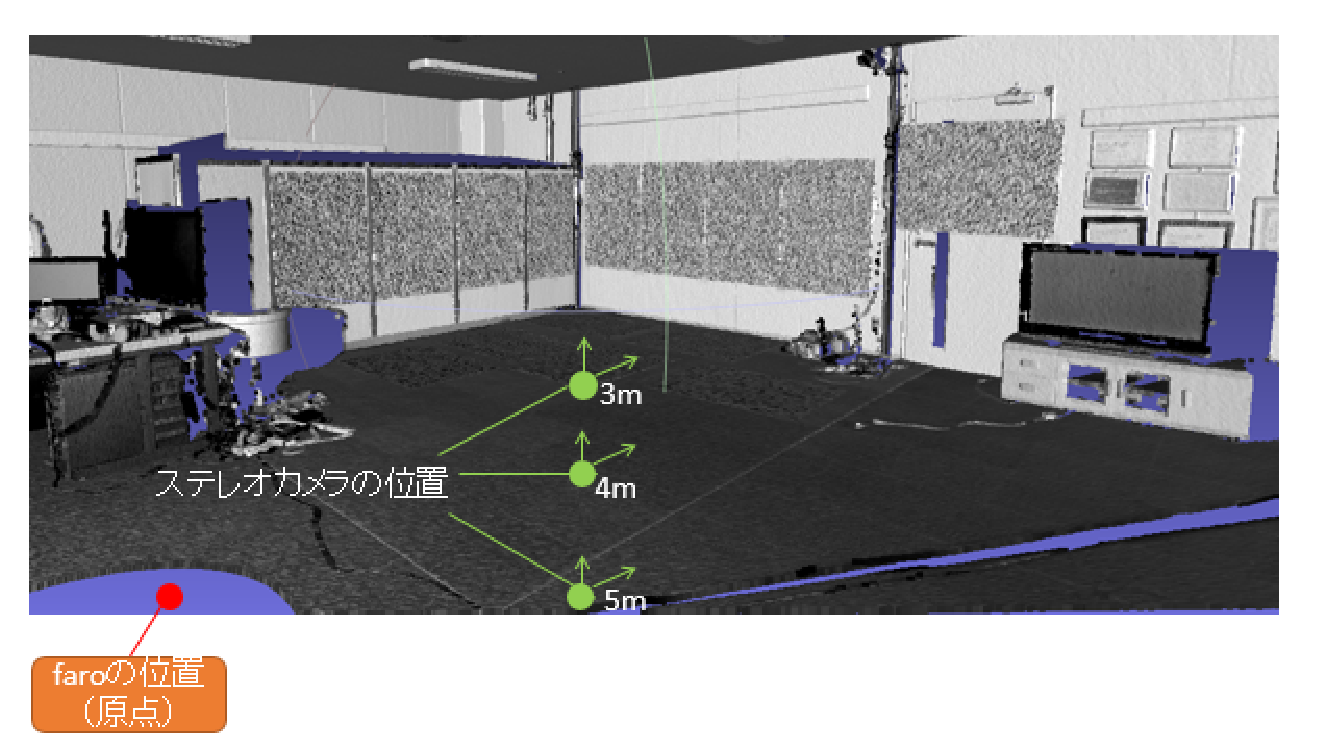
\includegraphics[height=80mm]{figure/テクスチャー有の屋内実験場所.eps}
   \caption{テクスチャー有の屋内実験場所}
   \label{テクスチャー有の屋内実験場所}
  \end{center}
\end{figure}

\begin{figure}[htbp]
  \begin{center}
   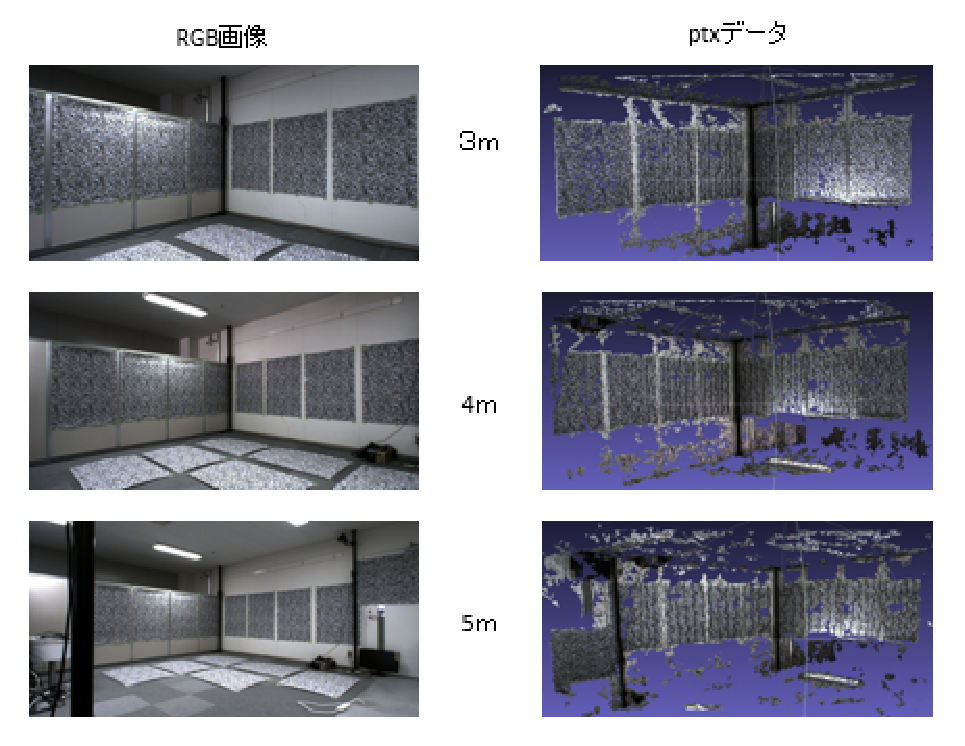
\includegraphics[height=90mm]{figure/テクスチャー有の屋内データ例.eps}
   \caption{テクスチャー有の屋内データ例}
   \label{テクスチャー有の屋内データ例}
  \end{center}
\end{figure}

\vspace{10mm}
テクスチャー有の屋内位置同定実験もテクスチャー無の屋内実験と同様に乱数を与えているため,毎回同じ位置に収束とは限らない.地図データと計測データとの収束性能も5回ずつ繰り返し位置同定を行い,台車の真位置から50cm以内で方向が10°以内の誤差であれば,成功とみなす.パラメータの調整対象もテクスチャー無の時と同様に,ボクセルサイズ80,40cmと地図・計測データのオーバーラップの有無となる.テクスチャー有の屋内位置同定結果をパラメータ毎に図4.14,図4.15に表す.

%
\begin{figure}[htbp]
  \begin{center}
   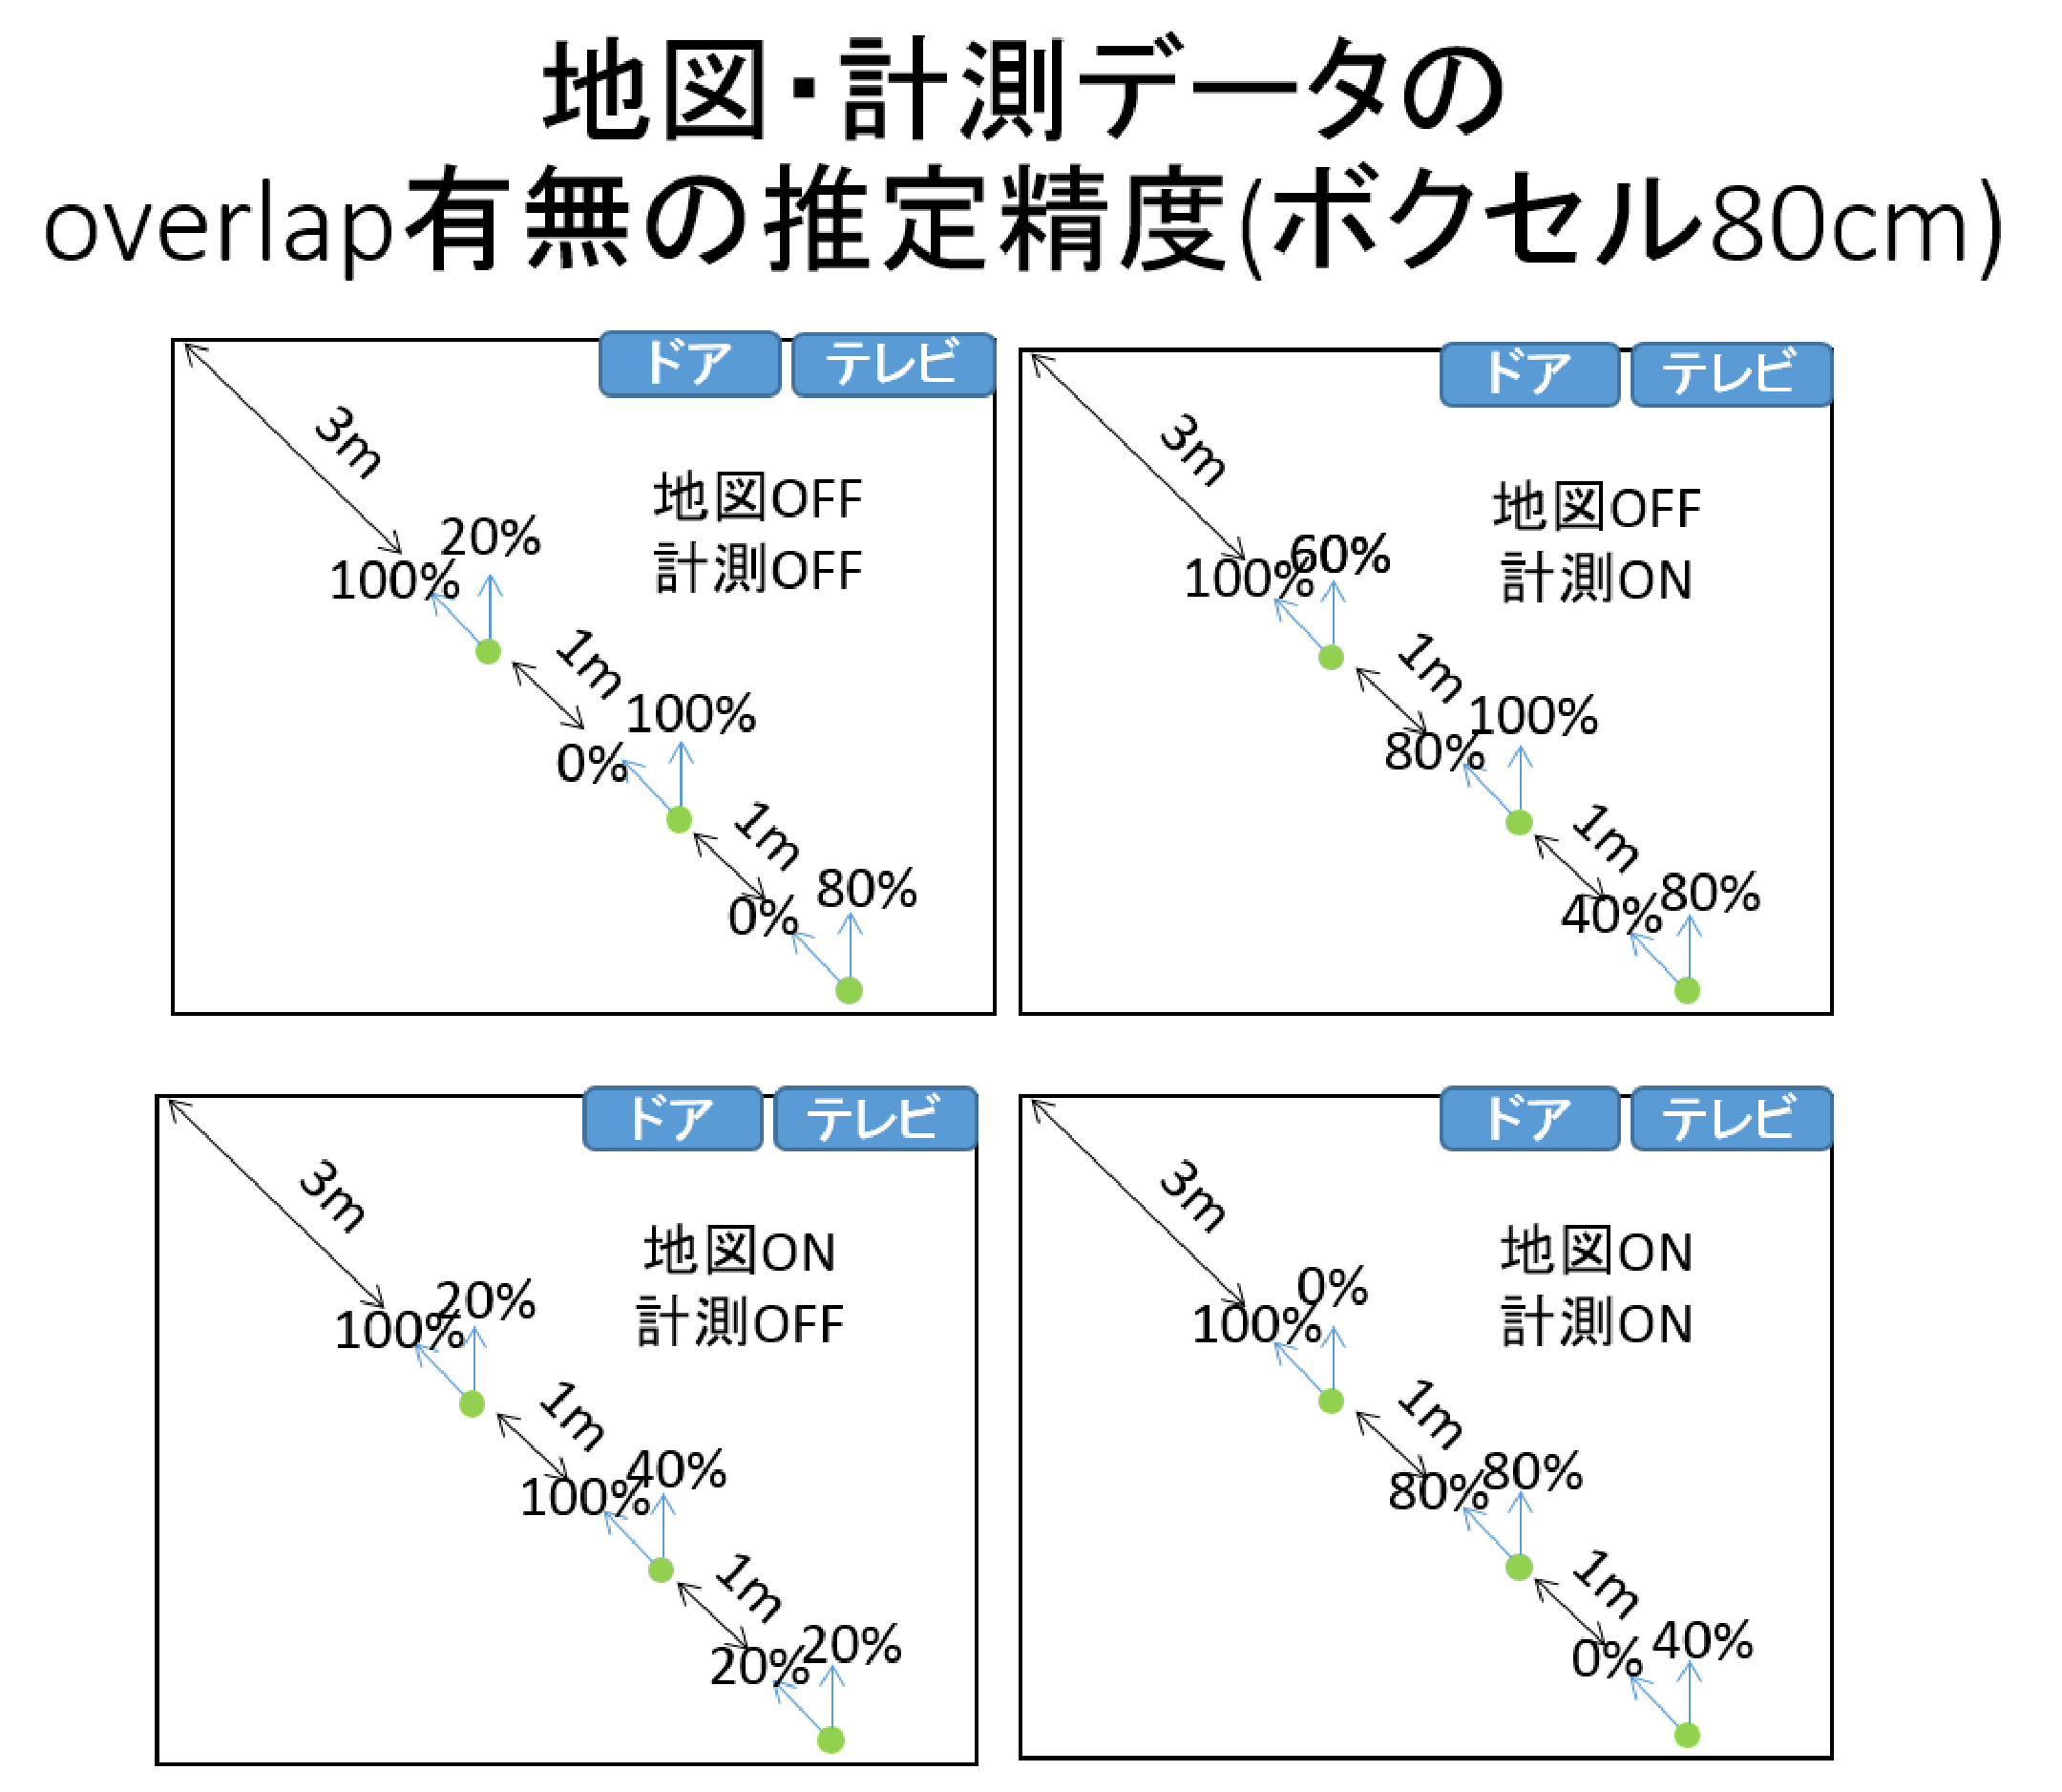
\includegraphics[height=60mm]{figure/有80.eps}
   \caption{テクスチャー有かつボクセルサイズ:80cm}
   \label{80-0}
  \end{center}
\end{figure}
%

%
\begin{figure}[htbp]
  \begin{center}
   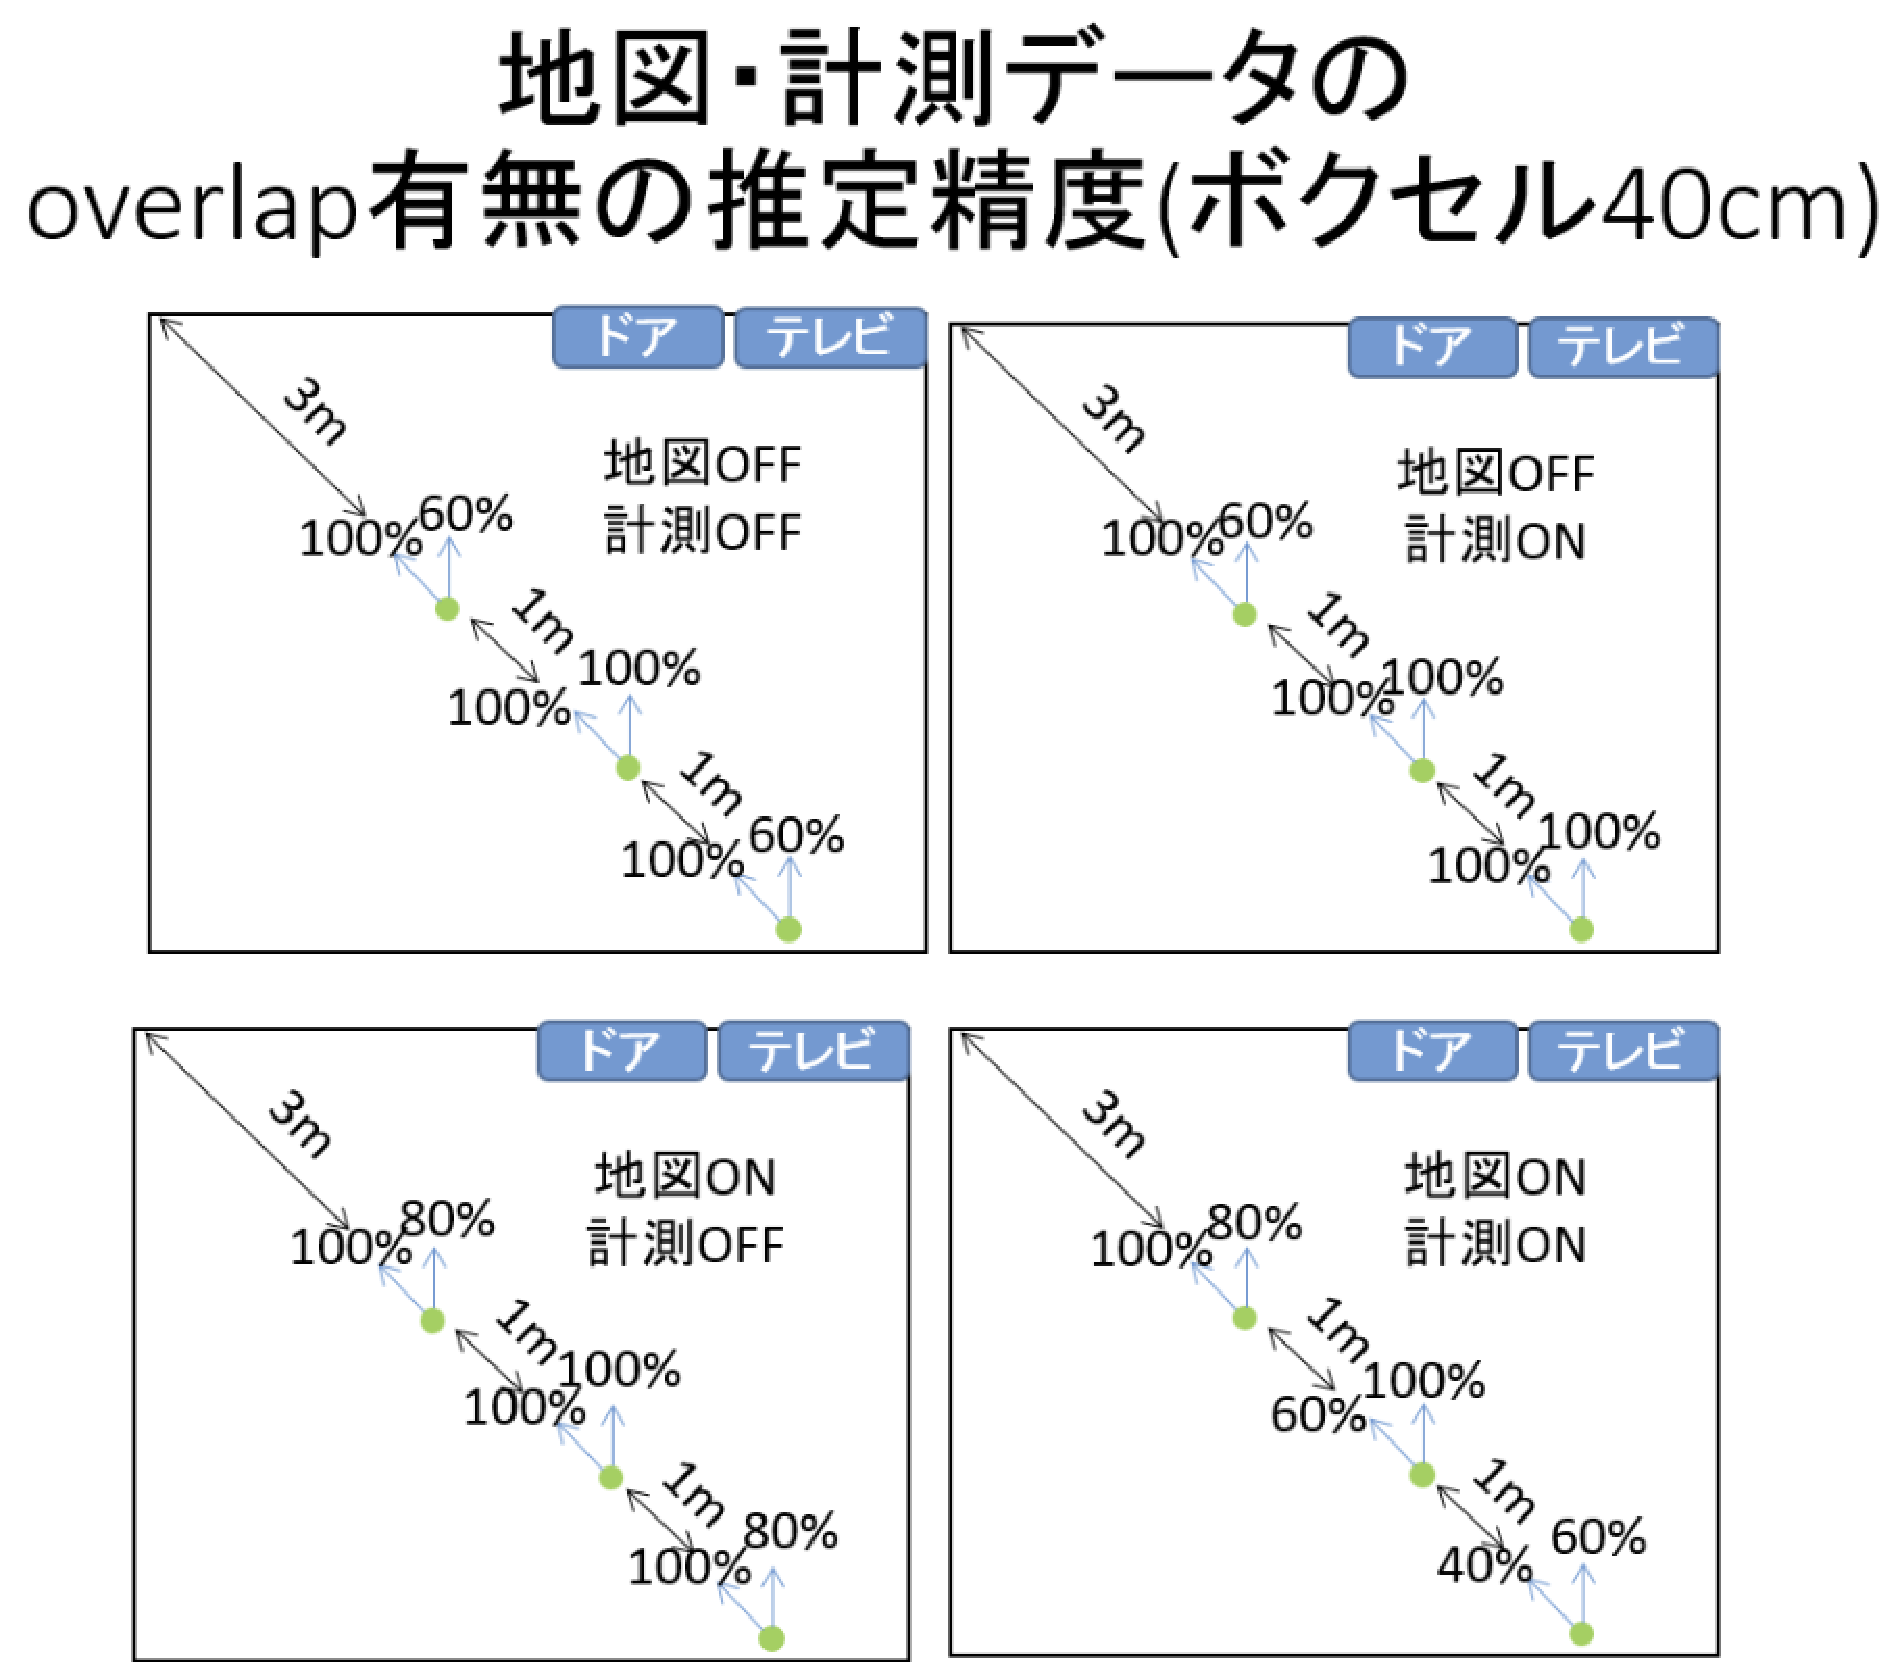
\includegraphics[height=60mm]{figure/有40.eps}
   \caption{テクスチャー有かつボクセルサイズ:40cm}
   \label{80-1}
  \end{center}
\end{figure}
%

\newpage

図4.14と図4.15を見ると,テクスチャー無の結果と同様にボクセルサイズが小さくなると,精度が良くなることが分かる.テクスチャー有の結果を用いてテクスチャー無の結果と同様に,条件毎に収束性能・パーティクル更新時間を数値にまとめた表を以下に表す.

%
\begin{figure}[htbp]
\begin{center}
\begin{tabular}{ccc} \hline
条件 & 収束性能(\%) &  パーティクル更新時間(ms)\\ \hline \hline
80-0-0 & 50 & 0.038\\ \hline
80-0-1 & 66.67 & 0.256\\ \hline
80-1-0 & 50 & 0.166\\ \hline
80-1-1 & 50 & 0.994\\ \hline
40-0-0 & 86.67 & 0.099\\ \hline
40-0-1 & 93.33 & 0.720\\ \hline
40-1-0 & 93.33 & 0.417\\ \hline
40-1-1 & 73.33 & 2.393\\ \hline
\end{tabular}
\end{center}
\end{figure}
%

上のデータから,速度と精度両方重視するのであれば,ボクセルサイズ40cmかつ地図・計測データオーバーラップ無が最も評価が良い.精度だけで比較すると,ボクセルサイズ40cmかつ地図データオーバーラップ無,計測オーバーラップ有が最も評価が良いことが分かる.各条件毎に収束性能・パーティクル更新時間を表したグラフを図4.16と図4.17に表す.\par
テクスチャー無とテクスチャー有のパーティクル更新時間を比較してみると,テクスチャー有の方がパーティクル更新時間が短い.テクスチャー有の方がより,点群がよく撮れているため,ボクセル数が多くてパーティクル更新時間が長いと予測されるが,予測と反対の結果が出ている.その理由と思われるのはデータを撮った場所の違いも挙げられるが,それよりテクスチャー無の方は特徴がばらばらに散らばっているため,ノイズなどを含めた点を計測された点と間違って認識し,無駄なボクセルを作っているためと思われる.実際に同じ条件,ボクセルサイズ80cmかつ地図・計測データオーバーラップ無の時,テクスチャー有のボクセル数は89であった反面,テクスチャー無のボクセル数は184であった.

%
\begin{figure}[htbp]
  \begin{center}
   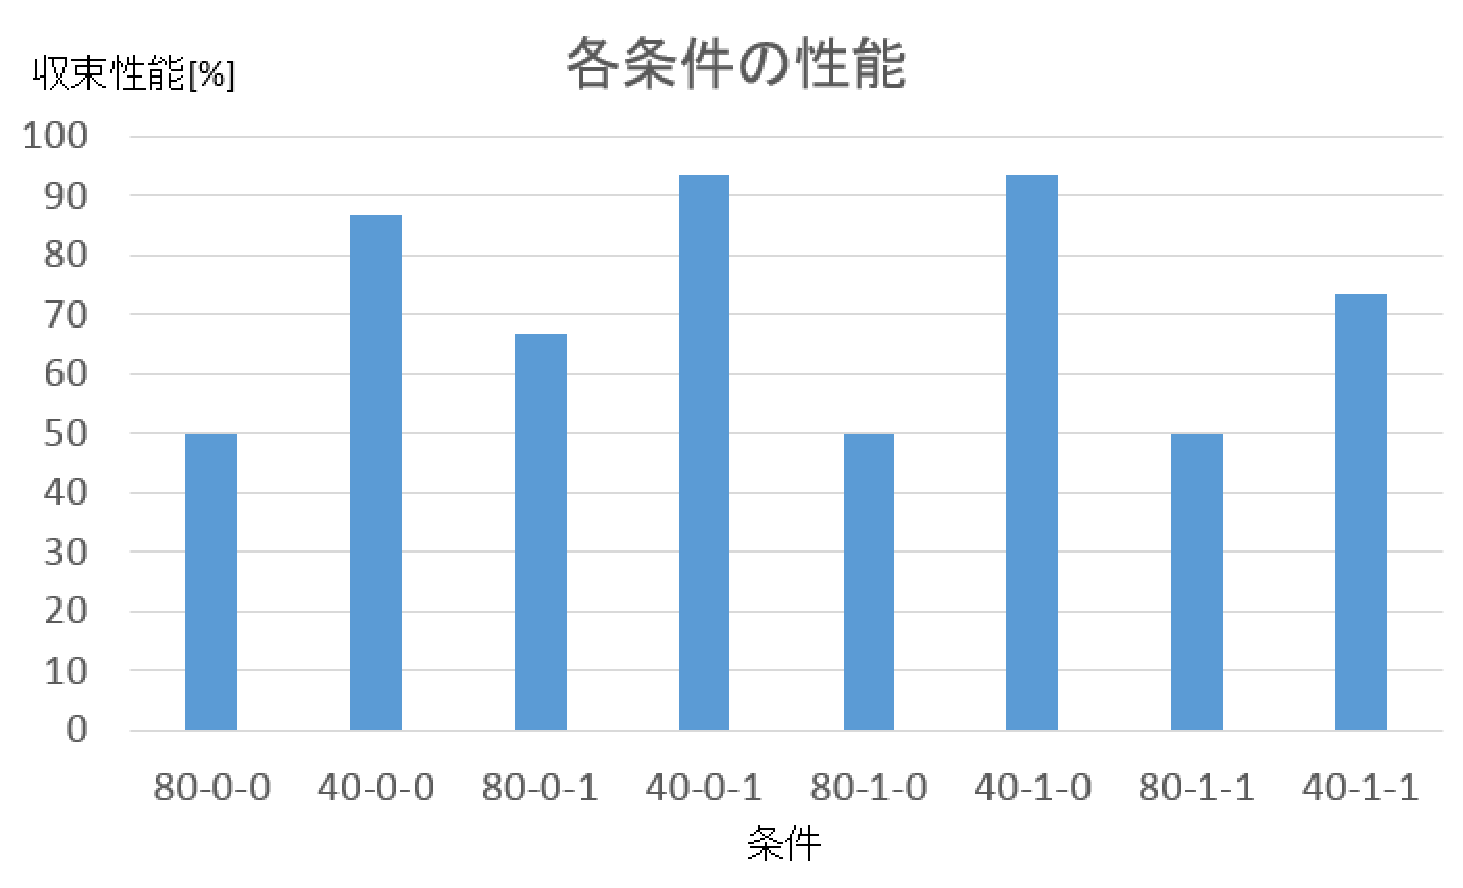
\includegraphics[height=80mm]{figure/各条件の性能2.eps}
   \caption{テクスチャー有の各条件の性能}
   \label{各条件の性能}
  \end{center}
\end{figure}
%

%
\begin{figure}[htbp]
  \begin{center}
   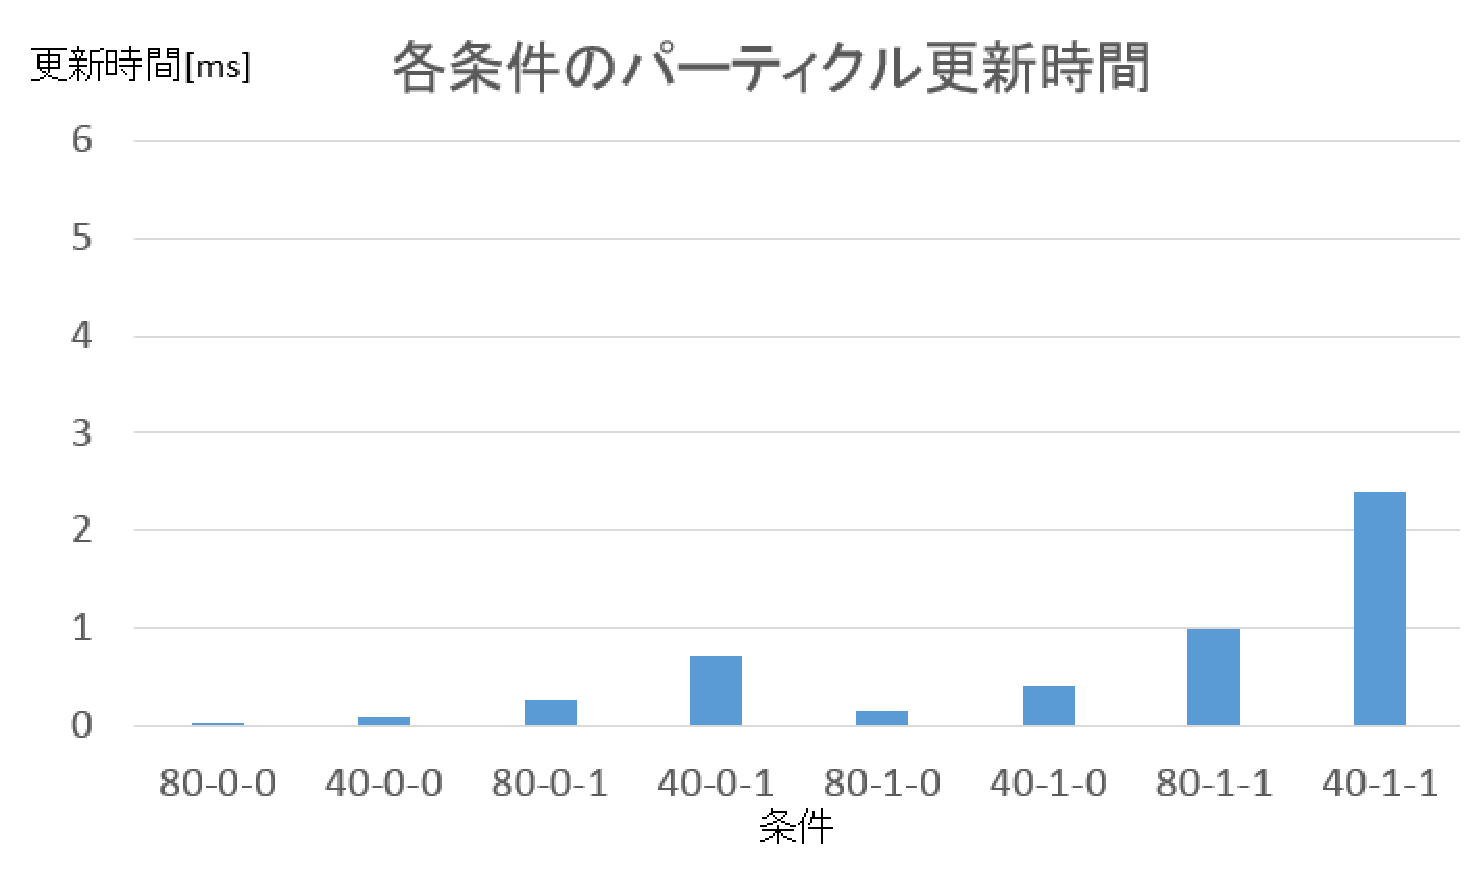
\includegraphics[height=80mm]{figure/各条件のパーティクル更新時間2.eps}
   \caption{テクスチャー有の各条件のパーティクル更新時間}
   \label{各条件のパーティクル更新時間}
  \end{center}
\end{figure}
%

\newpage
上のデータをより比較しやすくするために,ボクセルサイズ毎の地図データオーバーラップ無・計測データオーバーラップ無の時の収束性能・パーティクル更新時間を各々1とおいて,それに対する条件毎の比例数値を以下に表す.

%
\begin{figure}[htbp]
\begin{center}
\begin{tabular}{ccc} \hline
条件 & 収束性能(\%) &  パーティクル更新時間(ms)\\ \hline \hline
80-0-0 & 1 & 1\\ \hline
80-0-1 & 1.333 & 6.650\\ \hline
80-1-0 & 1 & 4.331\\ \hline
80-1-1 & 1 & 25.90\\ \hline \hline
40-0-0 & 1 & 1\\ \hline
40-0-1 & 1.077 & 7.298\\ \hline
40-1-0 & 1.077 & 4.224\\ \hline
40-1-1 & 0.846 & 24.24\\ \hline
\end{tabular}
\end{center}
\end{figure}
%

テクスチャー有無に関係なく,ボクセルサイズによる収束性能・パーティクル更新時間とボクセルサイズに関係なく,テクスチャー有無による収束性能を以下のように表す.左表の収束性能はテクスチャー有無の全てのプログラム実行回数の中,収束された確率で,パーティクル更新時間もテクスチャー有無の全ての条件でのパーティクル更新時間の平均である.右表の収束性能はボクセルサイズ(80,40cm)全てのプログラム実行回数の中で収束された確率である.ボクセルサイズが40cmになると,精度は29.49\%上がる反面,パーティクル更新時間は0.918ms遅くなる.また,テクスチャー有の場合がテクスチャー無の時より精度が37.36\%上がることが分かる.

\begin{table}[htbp]
\begin{center}
\begin{tabular}{|ccc||cc|} \hline
ボクセルサイズ(cm) & 収束性能(\%) &  パーティクル更新時間(ms) & テクスチャー有無 & 収束性能(\%)\\ \hline \hline
80 & 36.99 & 0.469 & 無 & 33.06\\ \hline
40 & 66.48 & 1.387 & 有 & 70.42\\ \hline
差 & 29.49 & 0.918 & 差 & 37.36\\ \hline
\end{tabular}
\end{center}
\end{table}

\newpage

より直感的に性能比較を行うために,収束性能を点数化して評価する.テクスチャー無とテクスチャー有の結果を各シーンで推定精度が80\%以上であれば3点,20\%~60\%であれば1点,0\%であれば0点として,換算した結果をまとめると表4.1と表4.2のようになる.

\begin{table}[htbp]
 \label{Tb:results}
  \begin{center}
    \begin{tabular}{|c|c|c|c|} \hline
	\multicolumn{1}{|c|} {\multirow{2}{*}{地図データ}}
	&\multicolumn{1}{c| }{\multirow{2}{*}{計測データ}}&\multicolumn{2}{c|}{ボクセルサイズ}\\ \cline{3-4}
      & & 40cm & 80cm \\ \hline
	& 有 & 25 & 15 \\ \cline{2-4}
	有 & 無 & 33 & 12 \\ \hline
       & 有 & 55 & 26 \\ \cline{2-4}
      無 & 無 & 49 &16  \\ \hline
    \end{tabular}
\caption{テクスチャー無のオーバーラップ有無による屋内定量評価の結果}
  \end{center}
\end{table}
\begin{table}[htbp]
 \label{Tb:results}
  \begin{center}
    \begin{tabular}{|c|c|c|c|} \hline
	\multicolumn{1}{|c|} {\multirow{2}{*}{地図データ}}
	&\multicolumn{1}{c| }{\multirow{2}{*}{計測データ}}&\multicolumn{2}{c|}{ボクセルサイズ}\\ \cline{3-4}
      & & 40cm & 80cm \\ \hline
	& 有 & 12 & 10 \\ \cline{2-4}
	有 & 無 & 16 & 10 \\ \hline
       & 有 & 16 & 14 \\ \cline{2-4}
      無 & 無 & 14 &10  \\ \hline
    \end{tabular}
 \caption{テクスチャー有のオーバーラップ有無による屋内定量評価の結果}
  \end{center}
\end{table}

テクスチャー有無の関係によらず,ボクセルサイズ400かつ地図データオーバーラップ無,計測データオーバーラップ有の時が最も精度良いが,前の計算時間の結果を考量すると最も有力な設定はボクセルサイズ400かつ地図データオーバーラップ無,計測データオーバーラップ無となる.この結果を踏まえて屋外の位置同定設定はボクセルサイズ400かつ地図データオーバーラップ無,計測データオーバーラップ無の状態とする.

\newpage

\subsection{ステレオカメラとKinect V2との比較実験・評価}
屋内位置同定に優れているKinect V2とステレオカメラを用いた位置同定比較実験を行う.実験場所はステレオカメラの精度が高い環境で実験するため,テクスチャー有の屋内実験場所と同じである.ステレオカメラとKinect V2は同じ台車の上でも図3.16のように違うところに置かれているため,球からKinect V2までの距離を物差しで測り,新しくKinect V2の真位置を求める.求めた真位置とKinect V2の計測データで位置同定を行った収束位置を比較し,収束性能を求める.図{\ref{ステレオカメラとKinectV2計測データ比較}}にステレオカメラとKinect V2の計測データ比較を表す.また,Kinect V2との収束性能を比較する実験のパラメータ設定はテクスチャー有のステレオカメラ収束性能の中で精度が良かったボクセルサイズ40cmかつ地図・計測データオーバーラップ無,ボクセルサイズ40cmかつ地図データオーバーラップ無,計測オーバーラップ有と2パターンにする.

%
\begin{figure}[htbp]
  \begin{center}
   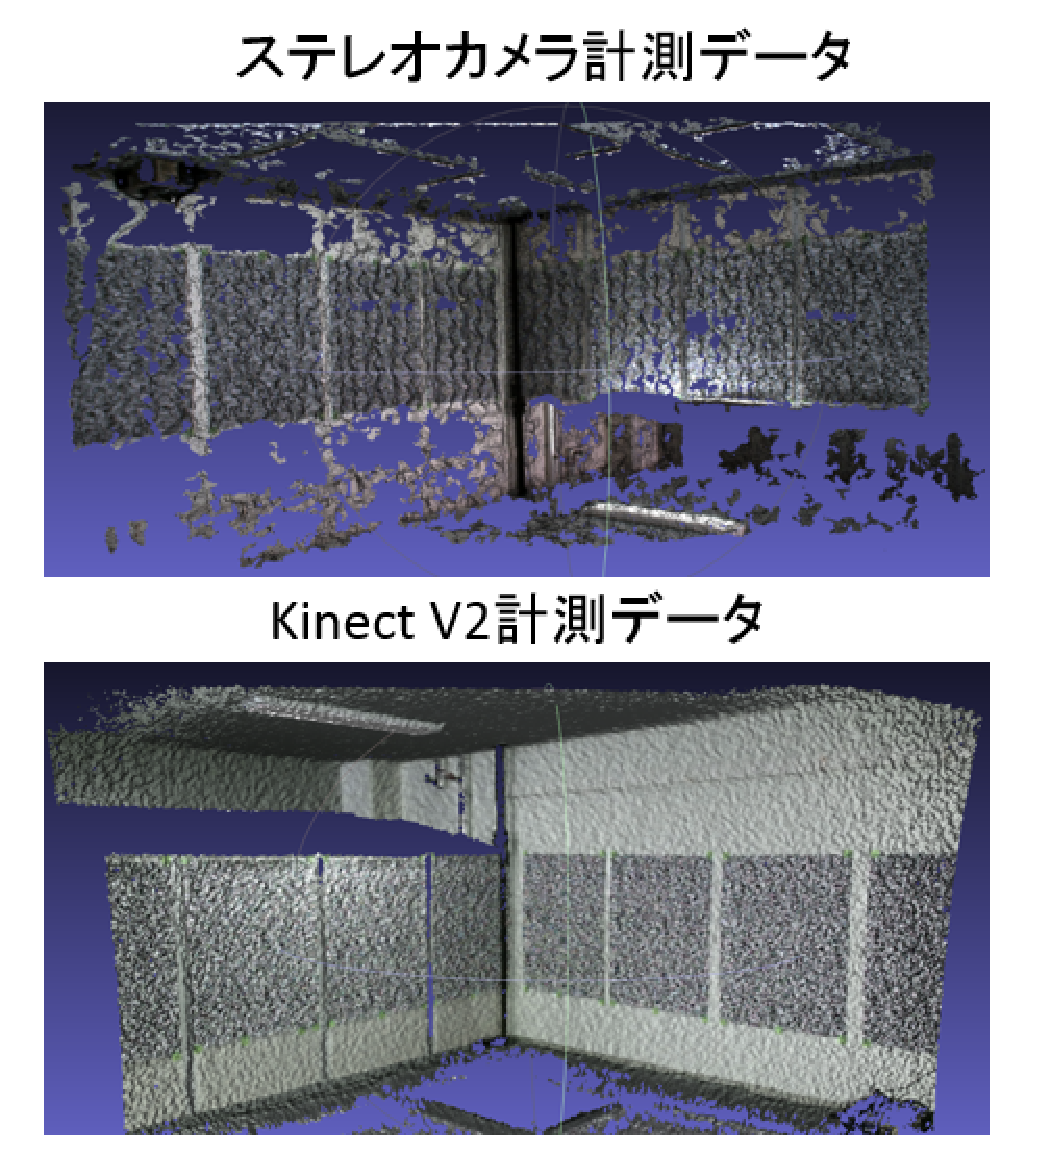
\includegraphics[height=100mm]{figure/ステレオカメラとKinectV2計測データ比較.eps}
   \caption{ステレオカメラとKinectV2計測データ比較例}
   \label{ステレオカメラとKinectV2計測データ比較}
  \end{center}
\end{figure}
%

\newpage

図{\ref{ステレオカメラとKinectV2計測データ比較}}から見ると,ステレオカメラの計測データはノイズが沢山含まれている反面,Kinect V2の計測データは綺麗に撮れていることが分かる.Kinect V2を用いて行った前述した2パターンの収束性能を図4.19に表す.図4.19から見ると,Kinect V2の位置同定精度は100\%である.Kinect V2とステレオカメラの位置同定精度を場所,パラメータ毎にまとめた結果を表4.3と表4.4に表す.

%
\begin{figure}[htbp]
  \begin{center}
   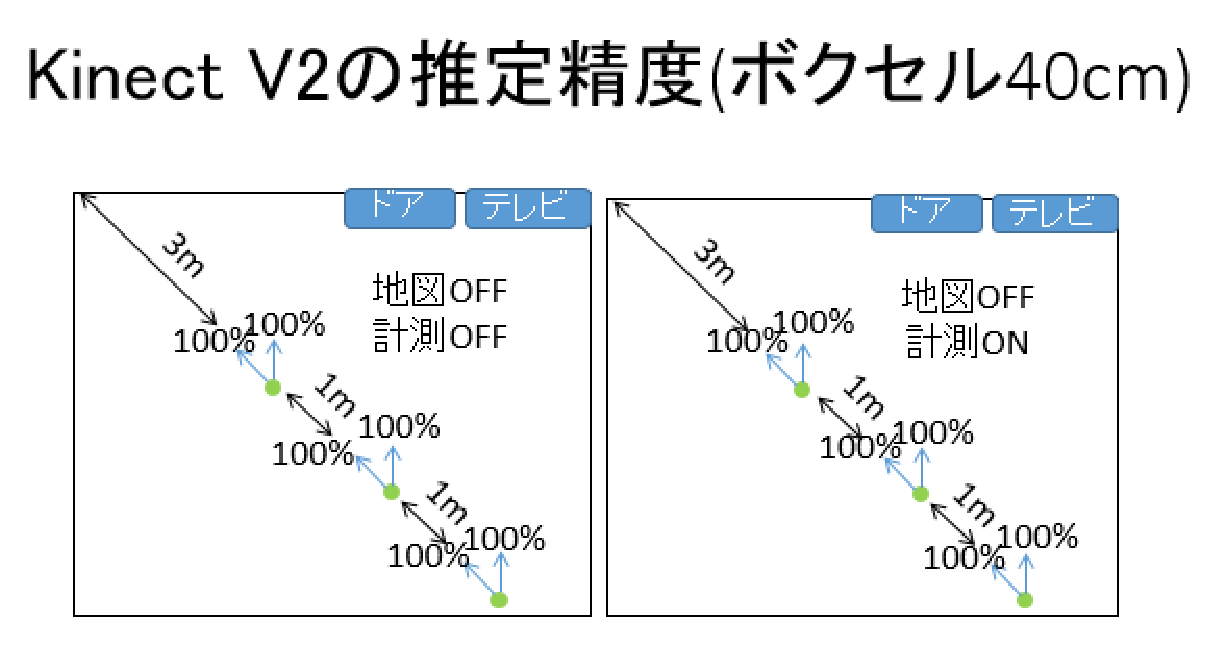
\includegraphics[height=50mm]{figure/KinectV2性能.eps}
   \caption{KinectV2 を用いた場合の収束性能}
   \label{KinectV2性能}
  \end{center}
\end{figure}
%

\begin{table}[htbp]
\begin{center}
\begin{tabular}{|c|c|c|} \hline
正面(m) & Kinect V2推定精度(m) & ステレオカメラの推定精度(m)\\ \hline
3 & 0.165 & 0.605 \\ \hline
4 & 0.110 & 0.202 \\ \hline
5 & 0.120 & 0.567 \\ \hline
平均 & 0.132 & 0.458 \\ \hline\hline
角(m) & Kinect V2推定精度(m) & ステレオカメラの推定精度(m)\\ \hline
3 & 0.112 & 0.108 \\ \hline
4 & 0.134 & 0.068 \\ \hline
5 & 0.148 & 0.105 \\ \hline
平均 & 0.131 & 0.094 \\ \hline
\end{tabular}
\caption{Kinect V2とステレオカメラの位置同定結果比較-ボクセルサイズ40cmかつ地図・計測データオーバーラップ無}
\end{center}
\end{table}

\begin{table}[htbp]
\begin{center}
\begin{tabular}{|c|c|c|} \hline
正面(m) & Kinect V2推定精度(m) & ステレオカメラの推定精度(m)\\ \hline
3 & 0.247 & 0.621 \\ \hline
4 & 0.105 & 0.313 \\ \hline
5 & 0.109 & 0.251 \\ \hline
平均 & 0.154 & 0.395 \\ \hline\hline
角(m) & Kinect V2推定精度(m) & ステレオカメラの推定精度(m)\\ \hline
3 & 0.130 & 0.190 \\ \hline
4 & 0.148 & 0.216 \\ \hline
5 & 0.135 & 0.285 \\ \hline
平均 & 0.138 & 0.230 \\ \hline
\end{tabular}
\caption{Kinect V2とステレオカメラの位置同定結果比較-ボクセルサイズ40cmかつ地図データオーバーラップ無,計測オーバーラップ有}
\end{center}
\end{table}

\newpage

表4.3と表4.4を見ると,ステレオカメラを用いて行う位置同定にはノイズが多く含まれているため,計測データのオーバーラップ有無に関係なく正面向きの壁から3mのところで誤差が大きく生じる.しかし,平均精度の結果を見ると,誤差が1ボクセルの単位である40cm近くであるため,ステレオカメラを用いた屋内の位置同定も,ある程度可能であることが分かる.また,角向きの計測データを用いたステレオカメラによる位置同定はKinect V2の精度にほぼ同じく推定できているため,ステレオカメラを用いた場合の収束性能は十分に高いと考えられる.
\newpage

%---------------------------------------------------------------------------------------------------
\section{屋外実験}
まず,ステレオカメラとRGB-Dカメラの日光の影響による収束性能の比較実験を行った.実験で使われるRGB-DカメラはKinect V2である.ステレオカメラとKinect V2を用いて同じ場所で昼,夕方,夜に分けてデータを撮り,データの比較を行う.次は,屋外位置同定実験・評価である.屋外実環境でステレオカメラを用いて位置同定の精度を確認する.今回屋外で実験を行った場所は九州大学伊都キャンパス図書館前である.最後に,一本の木を3方向から撮り,一本の木の特徴だけでも位置同定可能の有無を確認する実験を行い,評価する.
%---------------------------------------------------------------------------------------------------
\subsection{ステレオカメラとRGB-Dカメラの日光影響によるデータ比較}
まず,ステレオカメラとKinect V2の日光の影響によるデータ比較を行った.まず,計測データを撮った場所を図4.20に表す.実験場所は壁に特徴が多いところであり,距離データを取るため角向きとして行う.

%
\begin{figure}[htbp]
  \begin{center}
   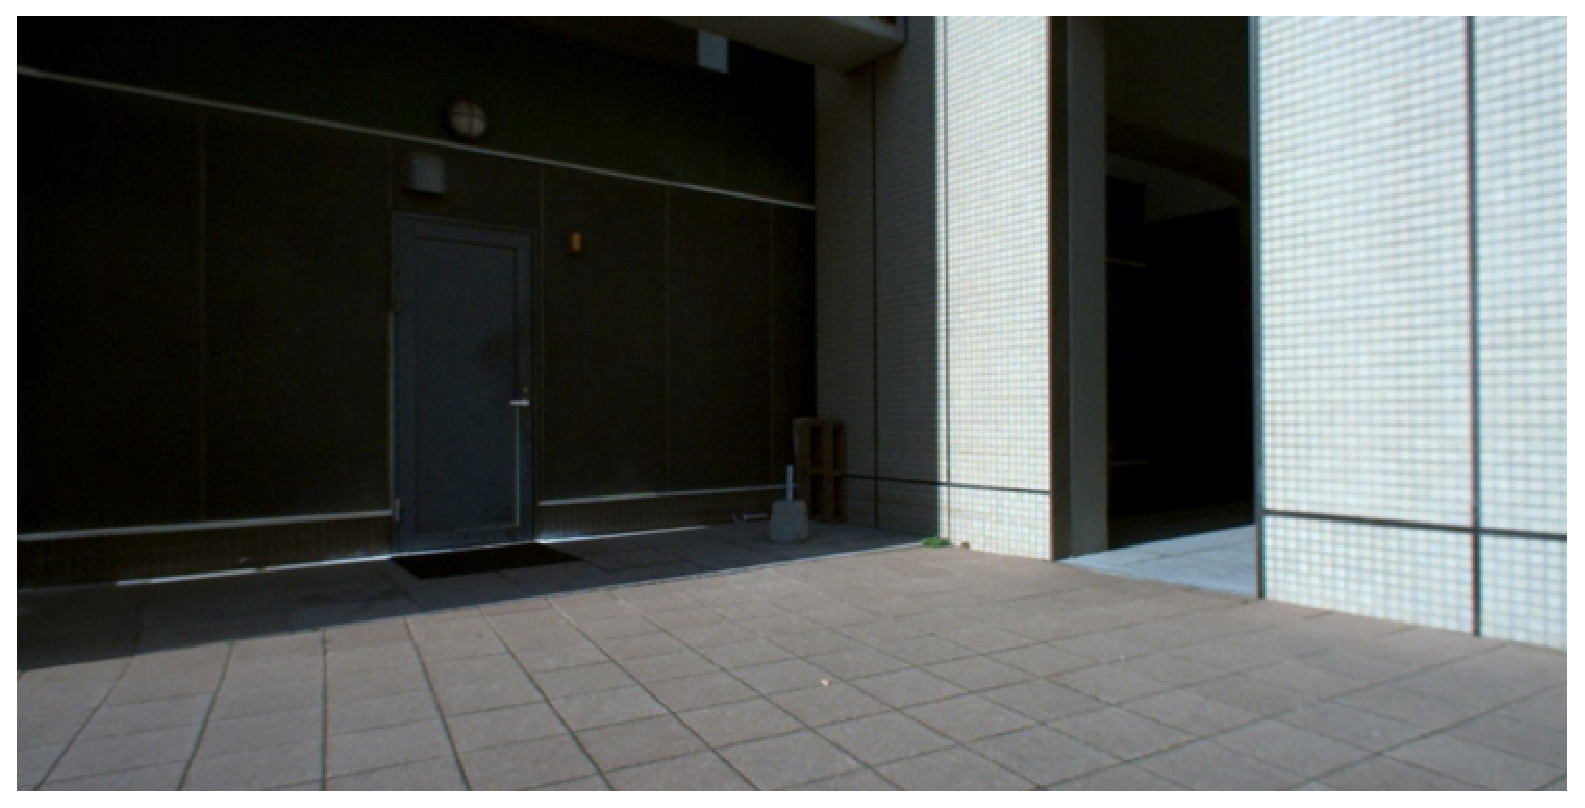
\includegraphics[height=80mm]{figure/日光影響によるデータ比較実実験場所.eps}
   \caption{日光影響によるデータ比較実実験場所}
   \label{日光影響によるデータ比較実実験場所}
  \end{center}
\end{figure}
%

\newpage

図4.20の実験場所で撮った昼,夕方,夜のステレオカメラ,Kinect V2のデータを図4.21に表す.

%
\begin{figure}[htbp]
  \begin{center}
   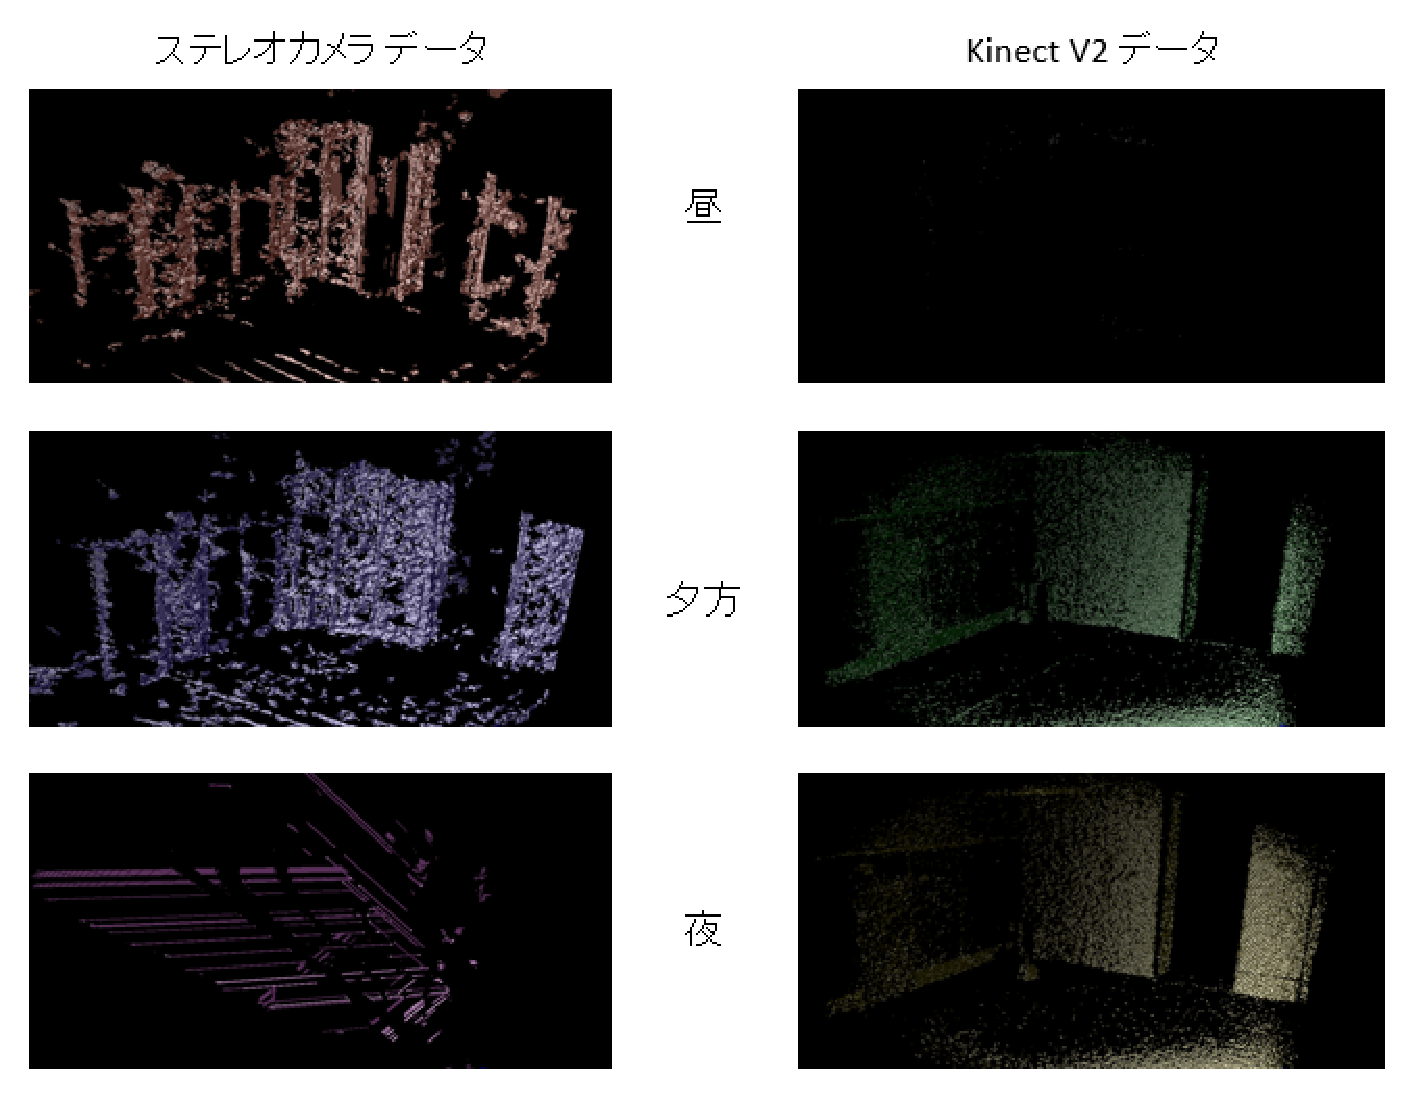
\includegraphics[height=120mm]{figure/日光影響によるデータ比較.eps}
   \caption{日光影響によるデータ比較}
   \label{日光影響によるデータ比較}
  \end{center}
\end{figure}
%

ステレオカメラとKinect V2の日光の影響によるデータ比較をすると,ステレオカメラは日が当たっている時であれば,データが綺麗に撮れている反面,Kinect V2は赤外線を用いたセンサであるため日が当たっているとデータが全然撮れていないことが分かる.しかし,日が沈んでKinect V2のレンズに日が当たっていなければ,Kinect V2データの方がより綺麗に撮れていることが分かる.ステレオカメラの夜データは後ろの壁の隙間から光が出ていたため,図4.21のような結果が出たと思われる.まとめると,屋外の位置同定は昼間や街灯など照明がある状況であれば,日光の影響や計測距離から,ステレオカメラの方がより適していることが分かる.
%---------------------------------------------------------------------------------------------------
\subsection{屋外位置同定実験・評価}
次は屋外の実環境でステレオカメラを用いた位置同定実験を行う.屋外位置同定実験は前述の通り,屋内評価の際に最も精度良くかつ高速なパターンであるボクセルサイズ40cmかつ地図・計測データオーバーラップ無に設定して行う.まず,実験を行った場所を図4.22に表す.\par
%
\begin{figure}[htbp]
  \begin{center}
   \includegraphics[height=80mm]{figure/屋外実験場所.eps}
   \caption{屋外実験場所}
   \label{屋外実験場所}
  \end{center}
\end{figure}
%
屋外実験を行ったルートは壁があるシーンと木々の間のシーンが撮れるルートの2つである.屋内実験実験とパラメータ条件はほぼ同じであるが,屋外の地図データは屋内に比べるとパーティクルをばら撒く範囲が広いため,台車の真値から半径3m以内にばら撒く範囲を固定して行う.ステレオカメラは性能上距離20mまで撮れるが,ノイズが多く含まれるため,本実験は計測データ10m以上のデータは捨てる.また,位置同定の結果は屋内位置同定と同様に5回繰り返し,x,y,z座標の平均誤差,平均距離誤差,平均方向誤差を各シーン毎に表す.
図4.23は10m以内に壁があるシーン(図4.22中の1-1)の各データを表し,また,表4.5に10m以内に壁があるシーンの位置同定結果を表す.同じく,図4.24には10m以内に壁がないシーン(図4.22中の1-3)の各データを表し,表4.6に10m以内に壁がないシーンの位置同定結果を表す.次は違うルートの木が2つあるシーン(図4.22中の2-1)の各データを図4.25に表し,表4.7に木が2つあるシーンの位置同定結果を表す.最後に,木とポールがあるシーン(図4.22中の2-3)の各データは図4.26に表し,表4.8に木とポールがあるシーンの位置同定結果を表す.


%
\begin{figure}[htbp]
  \begin{center}
   \includegraphics[height=50mm]{figure/10m以内に壁があるシーン.eps}
   \caption{10m以内に壁があるシーンの各データ}
   \label{10m以内に壁があるシーン}
  \end{center}
\end{figure}
%
\begin{table}[htbp]
\begin{center}
\begin{tabular}{|c|c|c|c|c|c|} \hline
\  & x(m) & y(m) & z(m) & 距離(m) & 方向(°)\\ \hline
平均誤差 & 0.08 & 0.17 & 0.08 & 0.21 & 2\\ \hline
\end{tabular}
\caption{10m以内に壁があるシーンの位置同定結果}
\end{center}
\end{table}
%
\begin{figure}[htbp]
  \begin{center}
   \includegraphics[height=50mm]{figure/10m以内に壁がないシーン.eps}
   \caption{10m以内に壁がないシーンの各データ}
   \label{10m以内に壁がないシーン}
  \end{center}
\end{figure}
%
\begin{table}[htbp]
\begin{center}
\begin{tabular}{|c|c|c|c|c|c|} \hline
\  & x(m) & y(m) & z(m) & 距離(m) & 方向(°)\\ \hline
平均誤差 & 1.22 & 1.81 & 0.00 & 2.31 & 155\\ \hline
\end{tabular}
\caption{10m以内に壁がないシーンの位置同定結果}
\end{center}
\end{table}
%
\begin{figure}[htbp]
  \begin{center}
   \includegraphics[height=50mm]{figure/木が2つあるシーン.eps}
   \caption{木が2つあるシーンの各データ}
   \label{木が2つあるシーン}
  \end{center}
\end{figure}
%
\begin{table}[htbp]
\begin{center}
\begin{tabular}{|c|c|c|c|c|c|} \hline
\  & x(m) & y(m) & z(m) & 距離(m) & 方向(°)\\ \hline
平均誤差 & 0.34 & 0.13 & 0.08 & 0.38 & 2.6\\ \hline
\end{tabular}
\caption{木が2つあるシーンの位置同定結果}
\end{center}
\end{table}
%
\begin{figure}[htbp]
  \begin{center}
   \includegraphics[height=50mm]{figure/木とポールがあるシーン.eps}
   \caption{木とポールがあるシーンの各データ}
   \label{木とポールがあるシーン}
  \end{center}
\end{figure}
%
\begin{table}[htbp]
\begin{center}
\begin{tabular}{|c|c|c|c|c|c|} \hline
\  & x(m) & y(m) & z(m) & 距離(m) & 方向(°)\\ \hline
平均誤差 & 1.24 & 1.68 & 0.09 & 2.1 & 156\\ \hline
\end{tabular}
\caption{木とポールがあるシーンの位置同定結果}
\end{center}
\end{table}
%

\newpage

図4.23の10m以内に壁があるシーンのステレオデータとボクセルデータから見ると,10m以内に壁のテクスチャーがあることと地面のテクスチャーも綺麗に撮れているため,平均誤差が小さい.しかし,図4.24の10m以内に壁がないシーンのデータを見ると,地面のテクスチャーだけで位置同定することになるため,平均誤差の結果から位置同定が難しいことが分かる.図4.25の木が2つあるシーンは2つの木と地面の特徴が撮れているため,このシーンに対する位置同定誤差は小さい.図4.26の木とポールがあるシーンは木,ポール,地面の特徴があるため,位置同定際の平均誤差が小さいと予測したが,位置同定ができていない.考えられる理由としては地図データを生成するFAROの位置から計測した位置までの間でオクルージョンがあり,オクルージョンの影響により点群が疎な木となっていると思われる.まとめると,屋外位置同定はランドマークとなるものが2つ以上でオクルージョンの影響がなければ,2つ以上のランドマークと地面の特徴を用いて位置同定することが可能である.

\subsection{一本の木に対する実験・評価}
一本の木と地面の特徴だけで,ステレオカメラを用いて位置同定が可能かを確かめた.位置同定するパラメータ設定と位置同定結果評価の方法は4.3.2の屋外位置同定実験と同様である.図{\ref{一本木の実験場所}}に一本木の実験を行った場所を表す.図{\ref{一本木の実験場所}}の赤い丸に囲まれている木を撮影する.また,緑の矢印が今回撮影を行った方向で,全3カ所0°,90°,180°のシーンである.
%
\begin{figure}[htbp]
  \begin{center}
   \includegraphics[height=70mm]{figure/一本木の実験場所.eps}
   \caption{一本木の実験場所}
   \label{一本木の実験場所}
  \end{center}
\end{figure}
%

\begin{figure}[htbp]
  \begin{center}
   \includegraphics[height=50mm]{figure/0°シーンの各データ.eps}
   \caption{0°シーンの各データ}
   \label{0°シーンの各データ}
  \end{center}
\end{figure}
%
\begin{table}[htbp]
\begin{center}
\begin{tabular}{|c|c|c|c|c|c|} \hline
\  & x(m) & y(m) & z(m) & 距離(m) & 方向(°)\\ \hline
平均誤差 & 0.7 & 0.18 & 0.03 & 0.72 & 1.2\\ \hline
\end{tabular}
\caption{0°シーンの位置同定結果}
\end{center}
\end{table}
%

\begin{figure}[htbp]
  \begin{center}
   \includegraphics[height=50mm]{figure/90°シーンの各データ.eps}
   \caption{90°シーンの各データ}
   \label{90°シーンの各データ}
  \end{center}
\end{figure}
%
\begin{table}[htbp]
\begin{center}
\begin{tabular}{|c|c|c|c|c|c|} \hline
\  & x(m) & y(m) & z(m) & 距離(m) & 方向(°)\\ \hline
平均誤差 & 0.77 & 2.61 & 0.25 & 2.73 & 146\\ \hline
\end{tabular}
\caption{90°シーンの位置同定結果}
\end{center}
\end{table}
%

\begin{figure}[htbp]
  \begin{center}
   \includegraphics[height=50mm]{figure/180°シーンの各データ.eps}
   \caption{180°シーンの各データ}
   \label{180°シーンの各データ}
  \end{center}
\end{figure}
%
\begin{table}[htbp]
\begin{center}
\begin{tabular}{|c|c|c|c|c|c|} \hline
\  & x(m) & y(m) & z(m) & 距離(m) & 方向(°)\\ \hline
平均誤差 & 0.45 & 0.45 & 0.02 & 0.64 & 7\\ \hline
\end{tabular}
\caption{180°シーンの位置同定結果}
\end{center}
\end{table}
%
\par
図4.28は0°シーンの各データを表し,また,表\hspace{-2mm}4.9に0°シーンの位置同定結果を表す.同じく,図\hspace{-2mm}4.29には90°シーンの各データを表し,表\hspace{-2mm}4.10には90°シーンの位置同定結果を表す.最後に,\hspace{-2mm}180°シーンの各データを図4.30に表し,表4.11に180°シーンの位置同定結果を表す.\par
一本の木の実験は一本だけの木と地面の特徴を用いて位置同定可能有無を確かめる実験であるため,計測データの中で他の木が写っている場合は,木のデータを消す.0°と\hspace{-2mm}180°のシーンを用いた位置同定結果の距離誤差は50cm以上,75cm以下であるが,特徴が一本木と地面しかないことと方向誤差が10°以下であることを踏まえると,ほぼ位置同定ができていると考えられる.しかし,90°のシーンを用いた位置同定では位置同定に失敗している.その理由としては計測データには撮れていないが,地図データを生成するFAROから90°シーンと似ているシーンが撮れているため,位置同定がそこの座標に収束していると思われる.
%===================================================================================================
% まとめと今後の課題
%===================================================================================================
\chapter{結論}
本研究では,従来の環境地図データとRGB-Dカメラの計測データを用いてNDTによる屋内位置同定する方法を拡張し,環境地図とステレオカメラの計測データを用いてNDTによる屋内・屋外位置同定する方法について検討した.
本論文では,まずNDTとパーティクルフィルタ,地図データと計測データとのマッチング評価について述べた.その後,位置同定実験の際に使われるステレオカメラの設定,ステレオカメラを搭載した実験用台車,環境地図について述べた.その後,実際に実験用台車とステレオカメラを用いて実験を行い,提案手法の性能を評価した.\par
本研究の実験は大きく屋内実験と屋外実験に分けられる.屋内実験では,壁に人為的にテクスチャ画像を張らない通常の環境で実験を行ったテクスチャー無の実験と,ステレオカメラの特徴をより認識しやすくするために行ったテクスチャー有の実験を行った.テクスチャー有無の実験を通して,ステレオカメラを用いて最も位置同定精度が高かったパラメータを求め,各々の精度評価を行った.実験の結果,最も精度良くかつ高速であるパラメーター設定は地図・計測データオーバーラップ無であることが分かった.また,求めたパラメータを用いて代表的なRGB-DカメラであるKinect V2との精度比較を行った.これらの実験を通して,ステレオカメラを用いたNDTによる屋内位置同定が可能であることを確認した.

屋内実験の今後の課題として挙げられるのは,精度と計算速度の向上である.最も精度良くかつ高速であるパラメーター設定は地図・計測データオーバーラップ無であるが,ボクセル40cmの場合リサンプリング100回の位置同定に所要される時間はテクスチャー無の場合33秒,テクスチャー有の場合19秒で,収束性能はテクスチャー無の場合59\%で,テクスチャー有の場合は86\%であった.テクスチャー有の方が点群が多いが,計算時間が短い理由はテクスチャー無の場合,不確実的な点とノイズが多いため,無駄なところに点群のボクセルができてしまい,計算速度が遅くなると思われる.これについては,無駄の点群からボクセルを生成しないようにプログラムを組むことで改善できる.また,Kinect V2を用いた屋内位置同定がステレオカメラを用いた屋内位置同定より性能が良いことから,データのノイズ除去などのステレオカメラの性能向上も課題として挙げられる.

屋外実験では,まず屋外の日光の影響によるステレオカメラ・Kinect V2のデータ比較実験を行った.これらのデータから,屋外の日光の影響によりKinect V2はデータが撮れていないが,光のない夜になると,ステレオカメラのデータが撮れていないことが確認できた.しかし,夜になっても光さえあると,ステレオカメラのデータは撮れるため,屋外位置同定はステレオカメラを用いた方が有利であることが確認できる.次に,ステレオカメラ・Kinect V2のデータ比較実験を基にして実屋外環境でのステレオカメラを用いた位置同定実験を行った.その結果,屋外位置同定はオクルージョンの影響がない条件で,ランドマーク2以上と地面の特徴が撮れていると位置同定可能であることが分かった.最後に一本木と地面の特徴だけで位置同定可能有無を確かめる実験を行った.一本木と地面だけの特徴を用いて位置同定する場合には,,計測データを撮る方向によって精度が大きく違うことが分かった.

屋外実験の今後の課題として挙げられるのは,屋内実験の課題と同様に精度と計算速度の向上である.本研究で用いるステレオカメラは距離20mまでデータが撮れるが,ノイズを沢山含むため,10m以上のデータは消している.10m以上のデータを消さずに,ノイズを除去し位置同定を行えると,精度と計算速度の向上が期待される.また,屋外の地図データはパーティクルをランダムにばら撒くのには広すぎるため,今回の屋外実験では計測場所の半径3m以内にパーティクルをばら撒いている.今は初期値を知っているため,初期値の周りにパーティクルを集中させ位置同定が可能であるが,パーティクルを屋外地図データ全体にばら撒いてからの位置同定の収束性能を確かめる必要がある.
%---------------------------------------------------------------------------------------------------
\acknowledgment
本論文を締めくくるに当たり,御指導を頂きました倉爪 亮教授, 諸岡准教授, 岩下准教授, 辻助教,河村助教に深く感謝致します.
特に,倉爪 亮教授,岩下准教授には,研究にあたり丁寧に御指導をして頂き,心より感謝致します.また,パナソニックの河村様,石上様,岡田様にも研究に当たり,丁寧にご指導をして頂き,深く感謝致します.研究室の皆様にも大変お世話になりました.特に,ホジョンさん,大音さんにはゼミに参加して頂き,本研究に関連する様々なアドバイスやお力添えを頂きました.心より感謝致します.
%---------------------------------------------------------------------------------------------------
\begin{thebibliography}{9}
\bibitem{shadow1}
	Jeong Yongjin, Ryo Kurazume, Yumi Iwashita and Tsutomu Hasegawa
	{\itshape "Global Localization for Mobile Robot using Large-scale 3D Environmental Map and RGB-D Camera",}
	 JRSJ, 2013.

\bibitem{shadow1}
	Jeong Yongjin, Shuji Oishi, Ryo Kurazume and Tsutomu Hasegawa
	{\itshape "Global localization by XOR voxel matching using RGB-D sensor and 3D map",}
	Proceedings of the 2012 JSME Conference on Robotics and Mechatronics, Hamamatsu, Japan, May 27-29, 2012 

\bibitem{shadow2}
	倉爪亮, 戸畑享大, 村上剛司, 長谷川勉
	{\itshape "CPS-SLAM の研究 大規模建造物の高精度3次元幾何形状レーザ計測システム",}
	日本ロボット学会誌, Vol. 25, No. 8, pp. 1234-1242, November 2007.

\bibitem{shadow3}
	Peter Biber and Wolfgang Straber
	{\itshape "The Normal Distributions Transform:A New Approach to Laser ScanMatching",}
	Proceedings of the 2003 IEEE/RSJ International Conference on Intelligent Robots and Systems, pp.
	2743-2748, 2003.

\bibitem{fisher_vector}
	Martin Magnusson, Henrik Andreasson, Andreas N$\ddot{u}$chter and Achim J. Lilienthal
	{\itshape "Automatic appearance-based loop detection from three-dimensional laser data using the normal distributions transform",}
	Journal of Field Robotics, Volume 26, Issue 11-12,  pages 892-914, November - December 2009
\bibitem{fisher_vector2}
	Cihan Ulas cihan and Hakan Temeltas hakan
	{\itshape "3D Multi-Layered Normal Distribution Transform for Fast and Long Range Scan Matching",} 
	Journal of Intelligent \& Robotic Systems, Volume 71, Issue1, pp 85-108 

\bibitem{vlad}
	Eijiro Takeuchi and Takashi Tsubouchi
	{\itshape "A Fast Scan Matching in 3-D Space using 3D Normal Distributions Transform toward Real-time 3-D Map Building",} 
	インテリジェントシステム・シンポジウム講演論文集, 2B2-1, 247-252
	
\end{thebibliography}
\end{document}\Uparrow